\documentclass{article}

\def\npart {IA}
\def\nterm {Michaelmas}
\def\nyear {2023}
\def\nlecturer {Prof H.\ Winton}
\def\ncourse {Groups}

\usepackage{alltt}
\usepackage{amsmath, amsfonts, amssymb, amsthm}
\usepackage{booktabs}
\usepackage{caption}
\usepackage{enumitem}
\usepackage{fancyhdr}
\usepackage{graphicx}
\usepackage{mathdots}
\usepackage{mathtools}
\usepackage{microtype}
\usepackage{multirow}
\usepackage{pdflscape}
\usepackage{pgfplots}
\usepackage{siunitx}
\usepackage{textcomp}
\usepackage{slashed}
\usepackage{tabularx}
\usepackage{tikz}
\usepackage{tkz-euclide}
\usepackage[normalem]{ulem}
\usepackage[all]{xy}

\pgfplotsset{compat=1.18}
\pagestyle{fancyplain}

\lhead{\emph{\nouppercase{\leftmark}}}
\rhead{
  \ifnum\thepage=1
  \else
    \npart\ \vline\ \ncourse
  \fi}

\def\nauthor{Marcus Ng}
\author{Based on lectures by \nlecturer \\\small Notes taken by \nauthor}
\date{\nterm\ \nyear}
\title{Part \npart\ --- \ncourse}

\newcommand*{\Cdot}{{\raisebox{-0.25ex}{\scalebox{1.5}{$\cdot$}}}}
\setlist[enumerate,1]{label={(\roman*)}}

\newcommand {\pd}[2][ ]{
  \ifx #1 { }
    \frac{\partial}{\partial #2}
  \else
    \frac{\partial^{#1}}{\partial #2^{#1}}
  \fi
}

% Theorems
\theoremstyle{definition}
\newtheorem*{aim}{Aim}
\newtheorem*{axiom}{Axiom}
\newtheorem*{claim}{Claim}
\newtheorem*{cor}{Corollary}
\newtheorem*{conjecture}{Conjecture}
\newtheorem*{defi}{Definition}
\newtheorem*{eg}{Example}
\newtheorem*{ex}{Exercise}
\newtheorem*{fact}{Fact}
\newtheorem*{law}{Law}
\newtheorem*{lemma}{Lemma}
\newtheorem*{notation}{Notation}
\newtheorem*{prop}{Proposition}
\newtheorem*{question}{Question}
\newtheorem*{problem}{Problem}
\newtheorem*{rrule}{Rule}
\newtheorem*{thm}{Theorem}
\newtheorem*{assumption}{Assumption}
\newtheorem*{assert}{Assertion}

\newtheorem*{remark}{Remark}
\newtheorem*{warning}{Warning}
\newtheorem*{exercise}{Exercise}

\newtheorem{nthm}{Theorem}[section]
\newtheorem{nlemma}[nthm]{Lemma}
\newtheorem{nprop}[nthm]{Proposition}
\newtheorem{ncor}[nthm]{Corollary}

\SetEnumitemKey{cases}{
  label=\underline{Case~\arabic*:},
  ref={\arabic*},
  align=left,
  leftmargin=\parindent
}

% \renewcommand{\labelitemi}{--}
% \renewcommand{\labelitemii}{$\circ$}
% \renewcommand{\labelenumi}{(\roman{*})}

\let\stdsection\section
\renewcommand\section{\newpage\stdsection}

% Strike through
\def\st{\bgroup \ULdepth=-.55ex \ULset}


%%%%%%%%%%%%%%%%%%%%%%%%%
%%%%% Maths Symbols %%%%%
%%%%%%%%%%%%%%%%%%%%%%%%%

% Logical symbols
\newcommand{\contradiction}{
  
\begin{tikzpicture}[rotate=45,x=0.5ex,y=0.5ex]
  \draw[line width=.1ex] (0,2) -- (3,2) (0,1) -- (3,1) (1,3) -- (1,0) (2,3) -- (2,0);
  \end{tikzpicture}
}


\let\U\relax
\let\C\relax
\let\G\relax

% Matrix groups
% \newcommand{\GL}{\mathrm{GL}}
% \newcommand{\Or}{\mathrm{O}}
% \newcommand{\PGL}{\mathrm{PGL}}
% \newcommand{\PSL}{\mathrm{PSL}}
% \newcommand{\PSO}{\mathrm{PSO}}
% \newcommand{\PSU}{\mathrm{PSU}}
% \newcommand{\SL}{\mathrm{SL}}
% \newcommand{\SO}{\mathrm{SO}}
% \newcommand{\Spin}{\mathrm{Spin}}
% \newcommand{\Sp}{\mathrm{Sp}}
% \newcommand{\SU}{\mathrm{SU}}
\newcommand{\U}{\mathrm{U}}
% \newcommand{\Mat}{\mathrm{Mat}}

% Matrix algebras
% \newcommand{\gl}{\mathfrak{gl}}
% \newcommand{\ort}{\mathfrak{o}}
% \newcommand{\so}{\mathfrak{so}}
% \newcommand{\su}{\mathfrak{su}}
% \newcommand{\uu}{\mathfrak{u}}
% \renewcommand{\sl}{\mathfrak{sl}}

% Special sets
\newcommand{\C}{\mathbb{C}}
\newcommand{\CP}{\mathbb{CP}}
\newcommand{\GG}{\mathbb{G}}
\newcommand{\N}{\mathbb{N}}
\newcommand{\Q}{\mathbb{Q}}
\newcommand{\R}{\mathbb{R}}
\newcommand{\RP}{\mathbb{RP}}
\newcommand{\T}{\mathbb{T}}
\newcommand{\Z}{\mathbb{Z}}
\renewcommand{\H}{\mathbb{H}}

% Brackets
\newcommand{\abs}[1]{\left\lvert #1\right\rvert}
\newcommand{\bket}[1]{\left\lvert #1\right\rangle}
\newcommand{\brak}[1]{\left\langle #1 \right\rvert}
\newcommand{\braket}[2]{\left\langle #1\middle\vert #2 \right\rangle}
\newcommand{\bra}{\langle}
\newcommand{\ket}{\rangle}
\newcommand{\norm}[1]{\left\lVert #1\right\rVert}
\newcommand{\normalorder}[1]{\mathop{:}\nolimits\!#1\!\mathop{:}\nolimits}
\newcommand{\tv}[1]{|#1|}
\renewcommand{\vec}[1]{\boldsymbol{\mathbf{#1}}}

% not-math
% \newcommand{\bolds}[1]{{\bfseries #1}}
% \newcommand{\cat}[1]{\mathsf{#1}}
% \newcommand{\ph}{\,\cdot\,}
% \newcommand{\term}[1]{\emph{#1}\index{#1}}
% \newcommand{\phantomeq}{\hphantom{{}={}}}

% Probability
% \DeclareMathOperator{\Bernoulli}{Bernoulli}
% \DeclareMathOperator{\betaD}{beta}
% \DeclareMathOperator{\bias}{bias}
% \DeclareMathOperator{\binomial}{binomial}
% \DeclareMathOperator{\corr}{corr}
% \DeclareMathOperator{\cov}{cov}
% \DeclareMathOperator{\gammaD}{gamma}
% \DeclareMathOperator{\mse}{mse}
% \DeclareMathOperator{\multinomial}{multinomial}
% \DeclareMathOperator{\Poisson}{Poisson}
% \DeclareMathOperator{\var}{var}
% \newcommand{\E}{\mathbb{E}}
% \newcommand{\Prob}{\mathbb{P}}

% Algebra
% \DeclareMathOperator{\adj}{adj}
% \DeclareMathOperator{\Ann}{Ann}
% \DeclareMathOperator{\Aut}{Aut}
% \DeclareMathOperator{\Char}{char}
% \DeclareMathOperator{\disc}{disc}
% \DeclareMathOperator{\dom}{dom}
% \DeclareMathOperator{\fix}{fix}
% \DeclareMathOperator{\Hom}{Hom}
% \DeclareMathOperator{\id}{id}
% \DeclareMathOperator{\image}{image}
% \DeclareMathOperator{\im}{im}
% \DeclareMathOperator{\re}{re}
% \DeclareMathOperator{\tr}{tr}
% \DeclareMathOperator{\Tr}{Tr}
% \newcommand{\Bilin}{\mathrm{Bilin}}
% \newcommand{\Frob}{\mathrm{Frob}}

% Others
% \newcommand\ad{\mathrm{ad}}
% \newcommand\Art{\mathrm{Art}}
% \newcommand{\B}{\mathcal{B}}
% \newcommand{\cU}{\mathcal{U}}
% \newcommand{\Der}{\mathrm{Der}}
% \newcommand{\D}{\mathrm{D}}
% \newcommand{\dR}{\mathrm{dR}}
% \newcommand{\exterior}{\mathchoice{{\textstyle\bigwedge}}{{\bigwedge}}{{\textstyle\wedge}}{{\scriptstyle\wedge}}}
% \newcommand{\F}{\mathbb{F}}
% \newcommand{\G}{\mathcal{G}}
% \newcommand{\Gr}{\mathrm{Gr}}
% \newcommand{\haut}{\mathrm{ht}}
% \newcommand{\Hol}{\mathrm{Hol}}
% \newcommand{\hol}{\mathfrak{hol}}
% \newcommand{\Id}{\mathrm{Id}}
% \newcommand{\lie}[1]{\mathfrak{#1}}
% \newcommand{\op}{\mathrm{op}}
% \newcommand{\Oc}{\mathcal{O}}
% \newcommand{\pr}{\mathrm{pr}}
% \newcommand{\Ps}{\mathcal{P}}
% \newcommand{\pt}{\mathrm{pt}}
% \newcommand{\qeq}{\mathrel{``{=}"}}
% \newcommand{\Rs}{\mathcal{R}}
% \newcommand{\Vect}{\mathrm{Vect}}
% \newcommand{\wsto}{\stackrel{\mathrm{w}^*}{\to}}
% \newcommand{\wt}{\mathrm{wt}}
% \newcommand{\wto}{\stackrel{\mathrm{w}}{\to}}
% \renewcommand{\d}{\mathrm{d}}
% \renewcommand{\P}{\mathbb{P}}
%\renewcommand{\F}{\mathcal{F}}

\let\Im\relax
\let\Re\relax

% \DeclareMathOperator{\area}{area}
% \DeclareMathOperator{\card}{card}
% \DeclareMathOperator{\ccl}{ccl}
% \DeclareMathOperator{\ch}{ch}
% \DeclareMathOperator{\cl}{cl}
% \DeclareMathOperator{\cls}{\overline{\mathrm{span}}}
% \DeclareMathOperator{\coker}{coker}
% \DeclareMathOperator{\conv}{conv}
% \DeclareMathOperator{\cosec}{cosec}
% \DeclareMathOperator{\cosech}{cosech}
% \DeclareMathOperator{\covol}{covol}
% \DeclareMathOperator{\diag}{diag}
% \DeclareMathOperator{\diam}{diam}
% \DeclareMathOperator{\Diff}{Diff}
% \DeclareMathOperator{\End}{End}
% \DeclareMathOperator{\energy}{energy}
% \DeclareMathOperator{\erfc}{erfc}
% \DeclareMathOperator{\erf}{erf}
% \DeclareMathOperator*{\esssup}{ess\,sup}
% \DeclareMathOperator{\ev}{ev}
% \DeclareMathOperator{\Ext}{Ext}
% \DeclareMathOperator{\fst}{fst}
% \DeclareMathOperator{\Fit}{Fit}
% \DeclareMathOperator{\Frac}{Frac}
% \DeclareMathOperator{\Gal}{Gal}
% \DeclareMathOperator{\gr}{gr}
% \DeclareMathOperator{\hcf}{hcf}
\DeclareMathOperator{\Im}{Im}
% \DeclareMathOperator{\Ind}{Ind}
% \DeclareMathOperator{\Int}{Int}
% \DeclareMathOperator{\Isom}{Isom}
% \DeclareMathOperator{\lcm}{lcm}
% \DeclareMathOperator{\length}{length}
% \DeclareMathOperator{\Lie}{Lie}
% \DeclareMathOperator{\like}{like}
% \DeclareMathOperator{\Lk}{Lk}
% \DeclareMathOperator{\Maps}{Maps}
% \DeclareMathOperator{\orb}{orb}
% \DeclareMathOperator{\ord}{ord}
% \DeclareMathOperator{\otp}{otp}
% \DeclareMathOperator{\poly}{poly}
% \DeclareMathOperator{\rank}{rank}
% \DeclareMathOperator{\rel}{rel}
% \DeclareMathOperator{\Rad}{Rad}
\DeclareMathOperator{\Re}{Re}
% \DeclareMathOperator*{\res}{res}
% \DeclareMathOperator{\Res}{Res}
% \DeclareMathOperator{\Ric}{Ric}
% \DeclareMathOperator{\rk}{rk}
% \DeclareMathOperator{\Rees}{Rees}
% \DeclareMathOperator{\Root}{Root}
% \DeclareMathOperator{\sech}{sech}
% \DeclareMathOperator{\sgn}{sgn}
% \DeclareMathOperator{\snd}{snd}
% \DeclareMathOperator{\Spec}{Spec}
% \DeclareMathOperator{\spn}{span}
% \DeclareMathOperator{\stab}{stab}
% \DeclareMathOperator{\St}{St}
% \DeclareMathOperator{\supp}{supp}
% \DeclareMathOperator{\Syl}{Syl}
% \DeclareMathOperator{\Sym}{Sym}
% \DeclareMathOperator{\vol}{vol}

\begin{document}
\maketitle{
    \small
    \noindent\textbf{Examples of groups}\\
    Axioms for groups. Examples from geometry: symmetry groups of regular polygons, cube, tetrahedron. Permutations on a set; the symmetric group. Subgroups and homomorphisms. Symmetry groups as subgroups of general permutation groups. The M\"obius group; cross-ratios, preservation of circles, the point at infinity. Conjugation. Fixed points of M\"obius maps and iteration.\hspace*{\fill} [4]

    \vspace{10pt}
    \noindent\textbf{Lagrange's theorem}\\
    Cosets. Lagrange's theorem. Groups of small order (up to order 8). Quaternions. Fermat-Euler theorem from the group-theoretic point of view.\hspace*{\fill} [5]

    \vspace{10pt}
    \noindent\textbf{Group actions}\\
    Group actions; orbits and stabilizers. Orbit-stabilizer theorem. Cayley's theorem (every group is isomorphic to a subgroup of a permutation group). Conjugacy classes. Cauchy's theorem.\hspace*{\fill} [4]

    \vspace{10pt}
    \noindent\textbf{Quotient groups}\\
    Normal subgroups, quotient groups and the isomorphism theorem.\hspace*{\fill} [4]

    \vspace{10pt}
    \noindent
    \textbf{Matrix groups}\\
    The general and special linear groups; relation with the M\"obius group. The orthogonal and special orthogonal groups. Proof (in $\R^3$) that every element of the orthogonal group is the product of reflections and every rotation in $\R^3$ has an axis. Basis change as an example of conjugation.\hspace*{\fill} [3]
    
    \vspace{10pt}
    \noindent\textbf{Permutations}\\
    Permutations, cycles and transpositions. The sign of a permutation. Conjugacy in $S_n$ and in $A_n$. Simple groups; simplicity of $A_5$.\hspace*{\fill} [4]}
    
\tableofcontents

%%%%%%%%%%%%%%%%%%%%%%
% Lecture 1: 5/10/2023
%%%%%%%%%%%%%%%%%%%%%%

\section{Examples and Definitions}

There are two ways of looking at groups; an algebraic approach that deals with equations and variables, and a geometric approach that looks at symmerties, tilings. etc. To begin we will consider the symmetries of shapes, and once we have a better idea of what a group can look like we will then begin to prove properties of groups algebraically.

Let's consider the plane symmetries of an equilateral triangle. For clarity sake, we will label each vertex with a number.
\begin{center}
    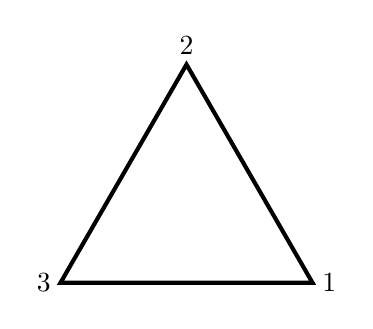
\begin{tikzpicture}[scale=0.8]
        \coordinate[label=left:$3$]  (A) at (0,0);
        \coordinate[label=right:$1$] (B) at (4,0);
        \coordinate[label=above:$2$] (C) at (2,3.464);
        
        \draw[line width=1.5pt] (A) -- (B) -- (C) -- cycle;
    \end{tikzpicture}
\end{center}

Given such a triangle, there are two main transformations we can make -- rotations and reflections. In total there are 6 such symmetries:
\begin{center}
    \begin{tabular}{ c c c }
        % Identity
        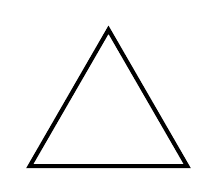
\begin{tikzpicture}
            \coordinate (A) at (0,0);
            \coordinate (B) at (2,0);
            \coordinate (C) at (1,1.732);
            
            \draw[line width=1.5pt] (A) -- (B) -- (C) -- cycle;
        \end{tikzpicture} 
        &
        % Left rotation
        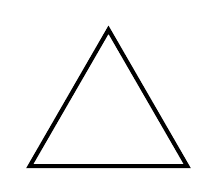
\begin{tikzpicture}
            \coordinate (A) at (0,0);
            \coordinate (B) at (2,0);
            \coordinate (C) at (1,1.732);
            
            \draw[line width=1.5pt] (A) -- (B) -- (C) -- cycle;
            
            % \draw[ultra thick, red, -{>[sep=2pt]}]
            %     (A) [left] edge [bend right=45] (B)
            %     (B) edge [bend right=45] (C)
            %     (C) edge [bend right=45] (A);
        \end{tikzpicture}
        &
        % Right rotation
        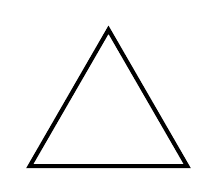
\begin{tikzpicture}
            \coordinate (A) at (0,0);
            \coordinate (B) at (2,0);
            \coordinate (C) at (1,1.732);
            
            \draw[line width=1.5pt] (A) -- (B) -- (C) -- cycle;
        \end{tikzpicture}
        \\
        % Top reflection
        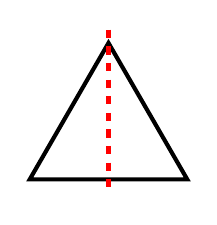
\begin{tikzpicture}
            \coordinate (A) at (0,0);
            \coordinate (B) at (2,0);
            \coordinate (C) at (1,1.732);
            
            \draw[line width=1.5pt] (A) -- (B) -- (C) -- cycle;

            \draw[red, dashed, line width=1.5pt] (1, 1.9) -- (1, -0.2);
        \end{tikzpicture}
        &
        % Left reflection
        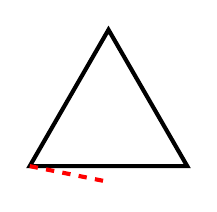
\begin{tikzpicture}
            \coordinate (A) at (0,0);
            \coordinate (B) at (2,0);
            \coordinate (C) at (1,1.732);
            
            \draw[line width=1.5pt] (A) -- (B) -- (C) -- cycle;

            \draw[red, dashed, line width=1.5pt] (0, 0) -- (1, -0.2);
        \end{tikzpicture}
        &
        % Right reflection
        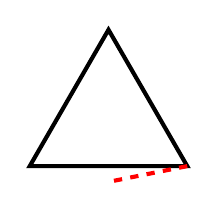
\begin{tikzpicture}
            \coordinate (A) at (0,0);
            \coordinate (B) at (2,0);
            \coordinate (C) at (1,1.732);
            
            \draw[line width=1.5pt] (A) -- (B) -- (C) -- cycle;

            \draw[red, dashed, line width=1.5pt] (2, 0) -- (1, -0.2);
        \end{tikzpicture}
    \end{tabular}
\end{center}

For each of these symmetries, we can compose or ``multiply'' them. For instance, we may perform a rotation followed by a reflection.

% Insert an image of three triangles to demonstrate composition

Firstly, notice that the result of two such composition is itself a symmertry. Specifically, it is the symmerty obtained by reflecting the trianlge by an axis that passes through the vertex $2$. There are three important features to note. 
\begin{enumerate}
    \item There is an identity (a symmetry that does nothing)
    \item Every symmetry has an inverse
    \item Symmerty multiplication is \emph{associative}
\end{enumerate}
Furthermore, there is an important non-feature; multiplication may not be commutative. In this case, performing a rotation followed by a reflection does not result in the same result as if the order of transformations were reversed. 

% Insert an image of three triangles to demonstrate non commutativity

\subsection{Algebra}

With the example in mind, we will now define what a group is algebraically. 

\begin{defi}[Binary Operation]
    A \emph{binary operation} on the set $X$ is a map
    \begin{align*}
        \cdot \ X \times X \rightarrow x \\
        (x, y) \longmapsto x \cdot y
    \end{align*}
\end{defi}

\begin{defi}[Group]
    A \emph{group} is a triple $(G, \cdot, e)$ where
    \begin{enumerate}
        \item $G$ is a set
        \item $\cdot$ is a binary operation
        \item $e \in G$
    \end{enumerate}

    Satisfying three Axioms
    \begin{enumerate}
        \item (Associativity) $\forall a, b, c \in G, \quad (a \cdot b) \cdot c = a \cdot (b \cdot c)$
        \item (Identity) $\forall a \in G, \quad a \cdot e = G$
        \item (Inverse) $\forall a \in G, \exists b \ \text{s.t.} \ a \cdot b = e$
    \end{enumerate}
\end{defi}

These axioms generalise the example encountered earlier.
\begin{eg}
    Consider the group $(\Z, +, 0)$

    We can show this forms a group as we have
    \begin{enumerate}
        \item (Associativity) since addition over the integers is associative
        \item (Identity) since $0$ acts as an additive identity
        \item (Inverse) since $\forall a \in \Z, \quad a + (-a) = 0$
    \end{enumerate}
\end{eg}
Now that we have established the axioms of groups we can prove some immediate properties.

\begin{prop}
    Let $(G, \cdot, e)$ be a group, and $a, b, b^{\prime}, e, e^{\prime} \in G$. Then,
    \begin{enumerate}
        \item if $a \cdot b = e$ then $b \cdot a = e$
        \item $e \cdot a = a$
        \item if $a \cdot b = e = a \cdot b^{\prime}$ then $b = b^{\prime}$
        \item if $a \cdot e^{\prime} = a$ then $e = e^{\prime}$
    \end{enumerate}
\end{prop}

\begin{proof}\leavevmode
    \begin{enumerate}
        \item We will show that inverses commute
        \begin{align*}
            b &= b \cdot e \tag{identity} \\
            &= b \cdot (a \cdot b) \tag{hypothesis} \\
            &= (b \cdot a) \cdot b \tag{associativity}
        \end{align*}

        By inverses, $\exists c \in G$ such that $b \cdot c = e$, so multiplying both sides of the equation on the right gives,

        \begin{align*}
            b \cdot c &= ((b \cdot a) \cdot b) \cdot c \\
            &= (b \cdot a) \cdot (b \cdot c) \tag{associativity} \\
            &= (b \cdot a) \cdot e \tag{identity}
        \end{align*}

        Hence, $e = b \cdot a$ as required
        
        \item We will show that left identity and the right identity are the same. By inverses and by part (i), $\exists b \in G$ such that $a \cdot b = e = b \cdot a$ 
        \begin{align*}
            e \cdot a &= (a \cdot b) \cdot A \\
            &= a \cdot (b \cdot a) \tag{associativity}\\
            &= a \cdot e \\
            &= a \tag{identity}
        \end{align*}

        \item We will show that multiplication is unique 
        \begin{align*}
            b^{\prime} &= e \cdot b^{\prime} \tag{ii}\\
            &= (b \cdot a) \cdot b^{\prime} \tag{i}\\
            &= b \cdot (a \cdot b^{\prime}) \tag{associativity}\\
            &= b \cdot e \tag{hypothesis} \\
            &= b \tag{identity}
        \end{align*}

        Alternatively, a for a stronger argument. $\exists c \in G$ such that $c \cdot a = e$
        \begin{align*}
            a \cdot b &= a \cdot b^{\prime} \\
            c \cdot (a \cdot b) &= c \cdot (a \cdot b^{\prime}) \\
            (c \cdot a) \cdot b &= (c \cdot a) \cdot b^{\prime} \tag{associativity} \\
            e \cdot b &= e \cdot b^{\prime} \\
            b &= b^{\prime} \tag{ii}
        \end{align*}

        \item We will show that identity is unique. By inverses and part (i), $\exists b \in G$ such that $b \cdot a = e$.
        \begin{align*}
            b \cdot a &= b \cdot (a \cdot e^{\prime}) \tag{hypothesis}\\
            &= (b \cdot a) \cdot e^{\prime} \tag{hypothesis}\\
            &= e \cdot e^{\prime} \\
            &= e^{\prime}
        \end{align*}
        
        Hence $e = e^{\prime}$
    \end{enumerate}
\end{proof}

%%%%%%%%%%%%%%%%%%%%%%
% Lecture 2: 7/10/2023
%%%%%%%%%%%%%%%%%%%%%%

Note that part (iii) says that inverses are \emph{unique}. Therefore, if $a \cdot b = e$. Firstly, we will introduce the superscript ``$-1$'' notation to indicate an inverse of some element. Then we can write
\begin{align*}
    b &= a^{-1} \\
    a \cdot a^{-1} &= e = a^{-1} \cdot a
\end{align*}

Therefore we have that the inverse of an inverse brings us back to the original element.
\[
    (a^{-1})^{-1} = a  
\]

Using this new notation, we can now define notation to write $\forall a \in G, \forall n \in \N$,
\begin{center}
    \begin{itemize}
        \item $a^0 = e$
        \item $a^1 = a$
        \item $a^2 = a \cdot a$
        \item[$\vdots$]
        \item $a^n = a^{n-1} \cdot a$
    \end{itemize}
\end{center}

We can also define negative exponentials as
\[
    a^n = (a^{-1})^{-n} \quad \text{for} \ n = -1, -2, -3, \ldots
\]

\begin{ex} Show that the following holds
    \begin{enumerate}
        \item $a^{m} \cdot a^{n} = a^{m + n}$
        \item $(a^{m})^{n} = a^{mn}$
    \end{enumerate}
\end{ex}
\begin{proof}\leavevmode
    \begin{enumerate}
        \item
        \begin{align*}
            a^m \cdot a^n &= a^m \cdot (a^{n-1} \cdot a) \tag{by definition} \\
            &= (a^m \cdot a) \cdot a^{n-1} \tag{associativity} \\
            &= a^{m+1} \cdot a^{n-1}
        \end{align*}

        Then we may proceed by induction, to arrive at
        \begin{align*}
            a^m \cdot a^n &= a^{m+n} \cdot a^{n-n} \\
            &= a^{m+n} \cdot a^0 \\
            &= a^{m+n} \cdot e \tag{by definition}\\
            &= a^{m+n} \tag{identity}
        \end{align*}
        
        \item
        \begin{align*}
            (a^m)^n &= (a^m)^{n-1} \cdot a^m \tag{by definition} \\
            &= ((a^m)^{n-2} \cdot a^m) \cdot a^m \\
            &= (a^m)^{n-2} \cdot (a^m \cdot a^m) \tag{associativity} \\
            &= (a^m)^{n-2} \cdot a^{2m} \tag{i} \\
        \end{align*}

        Then we may proceed by induction, to arrive at
        \begin{align*}
            (a^m)^n &= (a^m)^{0} \cdot a^{nm} \\
            &= e \cdot a^{nm} \tag{by definition} \\
            &= a^{nm} \tag{identity}
        \end{align*}
    \end{enumerate}
\end{proof}

\begin{remark}
    Recall that $a \cdot b$ is not necessarily $b \cdot a$ is a group $G$. So, we have to be careful when taking inverses after multiplying, the order of multiplication is reversed.
    \[
        (a \cdot b)^{-1} = b^{-1} \cdot a^{-1}  
    \]
\end{remark}

\begin{defi}[Abelian Group]
    If $(G, \cdot, e)$ is a group amd further satisfies that $a \cdot b = b \cdot a, \quad \forall a, b \in G$ then $G$ is called \emph{Abelian}
\end{defi}

\begin{defi}[Order of Group]
    The order of a group $(G, \cdot, e)$ is the number of elements of $G$, $\abs{G}$. If $\abs{G} < \infty$, then the group is finite
\end{defi}

\begin{eg}
    Here are some example and non-examples of groups
    \begin{enumerate}
        \item Trivial group. If $G = \{e\}$ and $e \cdot e = e$ then $(G, \cdot, e)$ is called the \emph{Trivial Group}
    \end{enumerate}
    Familiar examples from arithmetic
    \begin{enumerate}[resume]
        \item $(\Z, +, 0), (\Q, +, 0), (\R, +, 0), (\C, +, 0)$ as all abelian groups. In particular, the inverse of $x$ is $-x$
        \item $(\N, +, 0)$ is \emph{NOT} a group as there are no inverses
        \item $(\Q, \times, 1)$ is \emph{NOT} as group (0 does not have an inverse)
        \item $(\Q \setminus \{0\}, \times, 1), (\R \setminus \{0\}, \times, 1), (\C \setminus \{0\}, \times, 1)$ are abelian groups
    \end{enumerate}
    Finite examples
    \begin{enumerate}[resume]
        \item $\forall n \in \N, \ \text{let} \ C_n = \{z \in \C \mid z^n = 1\}$. Then $(c_n, \times, 1)$ forms an abelian group of order $n$
        \item Let $\Z_n = \{a \in \N \cup \{0\} \mid a < n\}$. Then for $a, b \in \Z_n$, let $a +_n b$ be the remainder when $a + b$ is divided by $n$. Then $(\Z_n, +_n, 0)$ form a group.
    \end{enumerate}
\end{eg}

%%%%%%%%%%%%%%%%%%%%%%
% Lecture 3: 10/10/2023
%%%%%%%%%%%%%%%%%%%%%%
\subsection{Matrix Groups and Symmetric Groups}
\begin{defi}[Matrix Group]
    Let $GL_2(\R)$ be the set of all $2 \times 2$ matrices
    \[
        A = \begin{pmatrix}
            a & b \\
            c & d
        \end{pmatrix} \quad \text{with} \quad a,b,c,d \in \R
    \]
    and $A$ is invertible i.e; $A$ has an inverse. $\exists B \in GL_2$ such that
    \[
        AB = \begin{pmatrix}
            1 & 0 \\
            0 & 1
        \end{pmatrix}
    \]
    Then $(GL_2(\R), \cdot, \begin{pmatrix}
        1 & 0 \\
        0 & 1
    \end{pmatrix})$ form a group
\end{defi}

From this definition we can see that this group is non-abelian -- as matrix multiplication is non-commutative, and that the group is infinite. For example, consider matrices of the form
\[
    \begin{pmatrix}
        1 & t \\
        0 & 1
    \end{pmatrix} \quad \forall t \in \R
\]

\begin{defi}[Symmetric Group]
    Let $X$ be a set. Then we define $\Sym(X)$ to be the set of all bijections from $X \rightarrow X$. 
    Alternatively we can think of this set as being the same as the set of all permutations of $X$.
    $\Sym(X)$ is called the symmetric group of $X$.
\end{defi}

\begin{defi}[$\Id_x$]
    The identity map, $\Id_x$ is defined as the map $x \mapsto x$. 
\end{defi}

\begin{lemma}[Compositive is associative]
    Consider maps $f, g, h$ of sets $w, x, y, z$
    \begin{center}
        \begin{tikzpicture}
            \graph {
                w ->["f"] x ->["g"] y ->["h"] z;
            };
        \end{tikzpicture}
    \end{center}
    Then $(h \circ g) \circ f = h \circ (g \circ f)$
\end{lemma}

\begin{proof}
    We will watch what happens to an element over the composed maps. Let $w \in W$
    \begin{align*}
        (h \circ g) \circ f (w) &= (h \circ g)(f(w)) \\
        &= h(g(f(w))) \\
        &= h(g \circ f(w)) \\
        &= h \circ (g \circ f)(w)
    \end{align*}
\end{proof}

\begin{prop}
    For any set $X, (\Sym(x), \circ, \Id_x)$ form a group
\end{prop}

\begin{proof}[Symmetric Group]
    To prove that $(\Sym(x), \circ, \Id_x)$ forms a group we need to show that
    \begin{enumerate}
        \item Associativity follows from the Lemma
        \item $\Id_x$ is the identity
        \item Inverses exist by the definition of bijection
    \end{enumerate}
\end{proof}

We are particularly interested in cases where $X$ is finite.
\begin{defi}[$S_n$]
    If $x = {1, 2, \cdots, n}$ then $S_n \equiv \Sym(X)$
\end{defi}

\begin{ex}
    What is the order of $S_n$?
\end{ex}

\begin{proof}
    The order of $S_n$ is equal to the number of permutations of $n$ elements and therefore $n!$
\end{proof}

\begin{remark}
    Before moving on, let's take note of the notation we are using. Currently, it takes a triple $(G, \cdot, e)$ to define a group. Moving forward, we will simply write $G$ to represent the whole group. However, when dealing with multiple groups, we will use $\cdot_G$ and $e_G$ to specify which binary operation and which identity belongs to the group $G$.
\end{remark}

\subsection{Subgroups}
\begin{defi}[Subgroup]
    Let $(G, \cdot_G, e_G)$ and $(H, \cdot_H, e_H)$ be groups. If
    \begin{enumerate}
        \item $H \subseteq G$
        \item $e_H = e_G$
        \item $\forall a, b \in H, \quad a \cdot_H b = a \cdot_G b$
    \end{enumerate}
    then $H$ is a \emph{subgroup} of $G$ and we write $H \leq G$
\end{defi}

\begin{prop}[Subgroup Criterion]
    Let $G$ be a group and $H \subseteq G$ be a non-empty subset. If
    \[
        \forall a, b \in H, \quad a \cdot_G b^-1 \in H
    \]
    then $H \leq G$
\end{prop}

\begin{proof}
    Since $H$ is nonempty, let $x \in H$. Therefore assuming the subgroup criterion,
    \begin{enumerate}
        \item (Identity) $x \cdot_G x^{-1} \in H \Rightarrow e_G \in H$
        \item (Inverse) $e_G \cdot_G a^{-1} \in H \Rightarrow a^{-1} \in H \quad \forall a \in H$
        \item (Closure) \begin{align*}
            \forall a, b \in H, b^{-1} \in H \tag{by Inverse} &\Rightarrow a \cdot_G (b^{-1})^{-1} \in H \\
            &\Rightarrow a \cdot_G b \in H
        \end{align*}
    \end{enumerate}
    Finally, if we set $\cdot_H =$ ``restriction of $\cdot_G$'' to $H$ and $e_H = e_G$ then $H \leq G$. 
\end{proof}

\begin{eg}\leavevmode
    \begin{enumerate}
        \item Every group $G$ is a subgroup of itself
        \item For every group $G$, $1_G = \{e_G\}$ is the Trivial subgroup
    \end{enumerate}
    Propper subgroups
    \begin{enumerate}[resume]
        \item $\Z \leq \Q \leq \R \leq \C$
        \item If $H_i \leq G$ for some set of $i$ then
        \[
            H = \bigcap_{i}{H_i} \leq G   
        \]
        is a subgroup.
        \item For any subset $X \subseteq G$, define
        \[
            \anglebk{X} = \bigcap_{X \subseteq H \leq G}{H} \leq G
        \]
        This is known as the subgroup \emph{generated} by $X$. In the case that $\anglebk{X} = G$ we say that $X$ \emph{generates} $G$
    \end{enumerate}
\end{eg}

\begin{ex}[Intersection of Subgroups]
    Prove statement (iv) that the intersection of subgroups is itself a subgroup. 
\end{ex}

\begin{proof}
    We will proceed by contradiction. Consider two elements $a, b \in H$. Since $H$ is the intersection of all $H_i$, $a, b \in H_i $ for all $i$.
    
    Suppose $b^{-1} \notin H$. Then, $\exists i$ such that $b^{-1} \notin H_i$. However, $H_i$ is a subgroup that fulfils the subgroup criterion. This is a contradiction \contradiction.

    Define $c \equiv a \cdot b^{-1}$. Suppose $c \notin H$. Then $\exists i$ such that $c \notin H_i$. However $H_i$ is a subgroup and must contain $c$ since it contains both $a$ and $b$. This is a contradiction \contradiction.
    
    Hence, $\forall a,b \in H, \quad a \cdot b^{-1} \in H \Rightarrow H \leq G$
\end{proof}

\begin{prop}
    The subgroups of $\Z$ are exactly the subsets
    \[
        n\Z = \{nk \in \Z \mid k \in \Z\} \quad \forall n = 0, 1, 2, \ldots
    \]
\end{prop}

%%%%%%%%%%%%%%%%%%%%%%
% Lecture 4: 12/10/2023
%%%%%%%%%%%%%%%%%%%%%%

\begin{proof}
    Note that each $n\Z$ is a subgroup of $\Z$. Applying the subgroup criterion, if
    \[
        a = nk, \quad b = nl \quad \text{for} \ k, l \in \Z  
    \]
    Then,
    \[
        a - b = n(k - l) \in n\Z  
    \]
    therefore each of $n\Z \leq Z$.

    Now suppose that for some subgroup $H \leq Z$. 
    If $H = \{0\}$, then $H = 0\Z$ and we have shown $H$ to be of the form $n\Z$.
    Otherwise, $H \neq \{0\}$ and we may choose some $n \in H \setminus \{0\}$ to be the smallest positive element of $H$. Since $H$ is closed under inverses,
    \[
        -n \in H  
    \]
    Since $H$ is closed under addition,
    \begin{align*}
        n + n = 2n &\in H \\
        2n + n = 3n &\in H \\
        &\vdots \\
        \forall k \in \Z^+, \ kn &\in H 
    \end{align*}
    Further,
    \begin{align*}
        -n - n = -2n &\in H \\
        -2n - n = -3n &\in H \\
        &\vdots \\
        \forall k \in \Z^-, \ kn &\in H 
    \end{align*}
    Therefore
    \[
        n\Z \leq H  
    \]
    We now want to show that $n\Z = H$. We will proceed by contradiction. Suppose $n\Z \neq H$, then $\exists x \in H$ such that $x \notin n\Z$. Using the division algorithm we can write
    \[
        x = nq + r, \quad \text{for} \ q \in \Z, \ 0 < r < n-1  
    \]
    Note that $r$ cannot be $0$ if not $x$ would belong in $n\Z$. Therefore
    \[
        r = x - qn  
    \]
    Note that since $x \in H$ and $qn \in H$, $r \in H$. However, $r$ would also be smaller than $x$. This is a contradiction \contradiction.
\end{proof}

\subsection{Geometric Examples}

Let $\C$ be the comoplex plane, equipped with the usual notaion of distance.

% insert diagram of complex plane

\begin{defi}[Isometry]
    For any subset $X \subseteq \C$, an \emph{isometry} of $X$ is an bijecetion $f: X \rightarrow X$ that preserves distance:
    \[
        \abs{f(x) - f(y)} = \abs{x - y}, \quad \forall x, y \in X
    \]
\end{defi}

\begin{prop}[Isometry Groups in $\C$]
    Let $X \subseteq \C$. The set of isometries of $X$,
    \[
        \Isom(X) = \{f: X \rightarrow X \mid f \ \text{is a bijection \& isometry}\}
    \]
    Then $\Isom(X)$ is a group with function composition and the identity map and it is a subgroup of $\Sym(X)$.
\end{prop}

\begin{proof}
    Since $\Id_x \in \Isom(X)$, $\Isom(X)$ is non-empty. By the subgroup criterion, it suffices to check that
    \[
        f \circ g^{-1} \in \Isom(X), \quad \text{for} \ f, g \in \Isom(X)   
    \]
    Let $x, y \in X$. Then,
    \begin{align*}
        \abs{f \circ g^{-1}(x) - f \circ g^{-1}(y)} &= \abs{g^{-1}(x) - g^{-1}(y)} \\
        &= \abs{g \circ g^{-1}(x) - g \circ g^{-1}(y)} \\
        & = \abs{x - y}
    \end{align*}
\end{proof}

\begin{defi}[Dihedral Groups]
    Let $X_n \subset \C$ be the $n$-gon with vertices written
    \[
        X_n = \{e^\frac{2\pi i k}{n} \mid k = 0, 1, \ldots, n-1 \}, \quad \text{for} \ n\geq 3
    \]
    Then we define the $n^{th}$ dihedral group as follows: (note the notation of using $2n$)
    \[
        \D_{2n} \equiv \Isom(X_n)
    \]
\end{defi}

\begin{eg}
    $\D_6$ is the isometry group of the equilateral triangle, and $\abs{\D_6} = 6$ 
\end{eg}

\begin{thm}[$\abs{\D_{2n}} = 2n$]
\end{thm}

We will first prove some lemmas from geometry

\begin{lemma}[Kite lemma]
    Let $x_1, x_2, y_1, y_2 \in \C$. If
    \begin{align*}
        \abs{y_1 - x_1} &= \abs{y_2 - x_1} \\
        \abs{y_1 - x_2} &= \abs{y_2 - x_2}
    \end{align*}
    Then, $x_2 - x_1$ is perpendicular to $y_2 - y_1$
\end{lemma}

\begin{proof}
    Excercise!
\end{proof}

\begin{lemma}[Three-point lemma]
    Let $x \subset \C$ and $f \in \Isom(x)$. If there are three points $x_1, x_2, x_3$ that are not colinear such that
    \[
        f(x_1) = x_1, \quad f(x_2) = x_2, \quad f(x_3) = x_3  
    \]
    then $f = \Id_x$
\end{lemma}
\begin{proof}
    We will proceed by contradiction. Suppose $\exists y \in X$ such that $f(y) \neq y$. Then,
    \begin{align*}
        \abs{f(y) - x_i} &= \abs{f(y) - f(x_i)} \\
        &= \abs{y - x_i}
    \end{align*}
    which will be true for $i = 1, 2, 3$.

    Let $y_1 = y$, and $y_2 = f(y)$. Then by the Kite lemma,
    \begin{align*}
        x_2 - x_1 &\perp f(y) - y \neq 0 \\
        x_3 - x_1 &\perp f(y) - y \neq 0
    \end{align*}
    Therefore, $x_1, x_2, x_3$ are colinear which is a contradiciton. \contradiction
\end{proof}

We will now show a stronger version, of the theorem stated earlier,
\begin{thm}[$\abs{\D_{2n}} = 2n$]
    If we define 2 elements in $\D_{2n}$
    \begin{enumerate}
        \item $r(z) = e^\frac{2 \pi i}{n} \cdot z$
        \item $s(z) = \overline{z}$
    \end{enumerate}
    Then,
    \[
        \D_{2n} = \{e, r, r^2, \ldots, r^{n-1}, s, rs, \ldots, r^{n-1}s\}  
    \]
\end{thm}

%%%%%%%%%%%%%%%%%%%%%%
% Lecture 5: 14/10/2023
%%%%%%%%%%%%%%%%%%%%%%

\begin{proof}
    First, we check that $r, s \in \D_{2n}$. Indeed, $\forall x, y \in \C$
    \begin{align*}
        \abs{r(x) - r(y)} &= \abs{e^\frac{2\pi i}{n}x - e^\frac{2\pi i}{n}y} \\
        &= \abs{e^\frac{2\pi i}{n}}\abs{x - y} \\
        &= \abs{x - y}
    \end{align*}
    Hence $r$ is an isometry. Furthermore,
    \[
        r(e^\frac{2\pi i k}{n}) =  e^\frac{2\pi i (k+1)}{n}
    \]
    Therefore $r$ preserves the polygon $X_n$. Similarly, $\forall x, y \in \C$
    \begin{align*}
        \abs{s(x) - s(y)} &= \abs{\overline{x} - \overline{y}} \\
        &= \abs{\overline{x - y}} \\
        &= \abs{x - y}
    \end{align*}
    Hence $s$ is an isometry. Furthermore,
    \[
        s(e^\frac{2\pi i k}{n}) =  e^{\frac{2\pi i}{n}(n - k)}
    \]
    Therefore $s$ preserves the polygon $X_n$, and hence $r, s \in \D_{2n}$.

    Now that we know that $r$ and $s$ are elements of $\D_{2n}$ we can get other element of $\D_{2n}$ by multiplying and taking inverses. This gives,
    \[
        \{e, r, r^2, \ldots, r^{n-1}, s, rs, \ldots, r^{n-1}s\} \subseteq \D_{2n}    
    \]
    To see that these are all the elements of $\D_{2n}$, let $f \in \D_{2n}$ be an arbitrary member. We will consider the action of $f$ on three points
    \[
        x = 1, \quad y = e^\frac{2\pi i}{n}, \quad z = e^\frac{-2\pi i k}{n}
    \]
    % insert diagram
    Note that we have $n \geq 3$ since these are the number of vertecies of a polygon. Therefore $x, y, z$ are non colinear. Since $f \in \D_{2n}$ it sends vertecies to vertecies, 
    \[
        f(z) = e^\frac{2\pi i k}{n} \quad \text{for some} k = 0, \cdots, n-1
    \]
    Therefore,
    \[
        r^{-k}\circ f(x) = 1 = x  
    \]
    Since $r^{-k}\circ f(z) \in \D_{2n}$,
    \begin{align*}
        r^{-k}\circ f(y) \in \{y, z\} \\
        r^{-k}\circ f(z) \in \{y, z\}
    \end{align*}
    Since these are mutually exclusive cases, we have two cases to consider
    \begin{enumerate}[cases]
        \item $r^{-k}\circ f(y) = y$ and $r^{-k}\circ f(z) = z$, therefore $r^{-k}\circ f$ fixes $x, y, z$ and by the three point lemma $ r^{-k}\circ f = \Id_x$, and by inverses $f = r^k$.
        \item $r^{-k}\circ f(y) = z$ and $r^{-k}\circ f(z) = y$ this is identical to
        \[
            x \mapsto x \quad y \mapsto s(y) \quad z \mapsto s(z)    
        \]
        therefore, by the three point lemma, $r^{-k}\circ f = s$ and therefore $s^{-1}r^{-k}\circ f = e$ fixes $x, y, z$. Therefore by inverses,
        \[
            f = r^ks  
        \]
    \end{enumerate}
    Therefore, all the elements in $\D_{2n}$ are of the form listed above. However, we have yet to show that all of the elements are distinct and $\abs{\D_{2n}} = 2n$. To do so we will consider the different cases,
    \begin{enumerate}[cases]
        \item if $0 \leq k, l < n$, $r^k = r^l$
        \begin{align*}
            r^k = e^\frac{2\pi i k}{n}(1) = e^\frac{2\pi i l}{n}(1) = r^l \\
            \Rightarrow k = l
        \end{align*}

        \item if $r^k = s$ then
        \begin{align*}
            e^\frac{2\pi i k}{n} = r^k(1) = s(1) = 1 \\
            \Rightarrow k = 0 \ \text{and} \ s = r^0 = e \quad \contradiction \\
            \therefore s \neq r^k \forall k
        \end{align*}

        \item if $r^k = r^ls$ then $s = r^{k-l}$ contradicting case 2
        \item if $0 \leq k, l < n$, $r^ks = r^ls$ then
        \begin{align*}
            \Rightarrow r^k = r^l \tag{multiply by $s^{-1}$} \\
            \Rightarrow k = l
        \end{align*}
    \end{enumerate}
\end{proof}

In order to understand how to multiply elements in $\D_{2n}$ we look at the Dihedral relation
\begin{lemma}[Dihedral Relations]
    For $r,s \in \D_{2n}$
    \[
        sr = r^{-1}s  
    \]
\end{lemma}

\begin{proof}
    To DO! using the three point lemma and the same set of ${x, y, z}$.
\end{proof}

\begin{eg}
    Lets do some algebra,
    \begin{itemize}
        \item $r^k \cdot r^l = r^{k + 1}$
        \item  $r^k \cdot r^ls = r^{k + 1}s$
        \item $(r^k \cdot s) r^l = r^{k - l}s$
        \item $r^k \cdot s \cdot r^l \cdot s= r^{k - l}ss = r^{k - l}$
    \end{itemize}
\end{eg}

All of the proofs that we have covered are not specific to $\C$, we could have done these in $\R^3$ similarly using a four point lemma.

\subsection{Homomorphisms}
\begin{defi}[Homomorphism]
    A map between groups $\phi: G \rightarrow H$ is called a homomorphism if $\forall g, g' \in G$
    \[
        \phi(g \cdot g') = \phi(g) \cdot \phi(g')  
    \]
\end{defi}

\begin{eg}\leavevmode
    \begin{enumerate}
        \item For any groups $G$ and $H$ the map 
        \begin{align*}
            \phi: G &\rightarrow H \\
            g &\mapsto e_H
        \end{align*}
        is the Trivial homomorphism

        \item if $H \leq G$ then the map
        \begin{align*}
            \phi: H &\rightarrow G \\
            h &\mapsto h
        \end{align*}
        is the Inclusion homomorphism

        \item Recall
        \[
            C_n = \{z_n \in \C \mid z^n = 1\}  
        \]
        if $n \mid m$ then
        \begin{align*}
            \phi: C_m &\rightarrow C_n \\
            z &\mapsto z^\frac{m}{n}
        \end{align*}
        is a homomorphism

        \item Since $\det(AB) = \det(A)\det(B)$ the map
        \begin{align*}
            \phi: GL_2(\R) &\rightarrow (\R \setminus \{0\}, \times, 1) \\
            A &\mapsto \det(A)
        \end{align*}
        is a homomorphism
    \end{enumerate}
\end{eg}

\begin{lemma}
    If $\phi: G \rightarrow H$ is a homomorphism
    \begin{enumerate}
        \item $\phi(e_G) = e_H$
        \item $\phi(g^{-1}) = \phi(g)^{-1}$ 
    \end{enumerate}
\end{lemma}

\begin{proof}\leavevmode
    \begin{enumerate}
        \item \begin{align*}
            e_H &= \phi(e_G)^{-1} \cdot \phi(e_G) \\
            &= \phi(e_G)^{-1} \cdot (\phi(e_G) \cdot \phi(e_G)) \tag{homomorphism property}\\
            &= (\phi(e_G)^{-1} \cdot \phi(e_G)) \cdot \phi(e_G) \\
            &= e_H \cdot \phi(e_G)
            &= \phi(e_G)
        \end{align*}
        \item \begin{align*}
            \phi(g) \cdot \phi(g^{-1}) &= \phi(g \cdot g^-1) \tag{homomorphism property} \\
            &= \phi(e_G) \\
            &= e_H \\
            \Rightarrow \phi(g^{-1}) &= \phi(g)^{-1}
        \end{align*}
    \end{enumerate}
\end{proof}

%%%%%%%%%%%%%%%%%%%%%%
% Lecture 6: 17/10/2023
%%%%%%%%%%%%%%%%%%%%%%

\begin{defi}[Isomorphism]
    If a homomorphism $\phi : G \rightarrow H$ is also a bijection, we say that $\phi$ is a \emph{Isomorphism} and we write
    \[
        G \cong H
    \]
\end{defi}

\begin{eg}\leavevmode
    \begin{enumerate}
        \item Recall $C_n = \{z \in C \mid Z^n = 1\}$ and $\Z_n = \{0, 1, 2, \cdots, n-1\}$. Then
        \begin{align*}
            \phi : \ \Z_n &\rightarrow C_n \\
            k &\mapsto e^\frac{2 \pi i k}{n}
        \end{align*}
        is a bijection. Let's check the homomorphism property. Recall the addition modulo $n$ operator
        \[
            k + l = pn + (k +_n l)  
        \]
        for some $p \in \Z$.
        \begin{align*}
            \phi(k +_n l) &= e^{\frac{2 \pi i}{n}(k +_n l)} \\
            &= e^{\frac{2 \pi i}{n}(pn)} \times e^{\frac{2 \pi i}{n}(k +_n l)} \\
            &= e^{\frac{2 \pi i}{n}(k + l)} \\
            &= e^{\frac{2 \pi i k}{n}} e^{\frac{2 \pi i l}{n}} \\
            &= \phi(k)\phi(l)
        \end{align*}
        
        \item Take the exponential function
        \begin{align*}
            \exp : \ (\R, +, 0) &\rightarrow (\R, \times, 1)\\
            x &\mapsto e^x
        \end{align*}
        is a homomorphism since $\exp(x + y) = \exp(x)\exp(y)$. Furthermore, since the inverse function exists, we have a bijection. Therefore $\exp$ is an isomorphism.
    \end{enumerate}
\end{eg}

\begin{lemma}\leavevmode
    \begin{enumerate}
        \item If $\phi : G \rightarrow H$ is an isomorphism, so is $\phi^{-1}$
        \item If $G \xrightarrow{\phi} H \xrightarrow{\psi} K$ are homomorphism, then so is $\psi \circ \phi$
        \item $\cong$ is an equivalence relation. That is
        \begin{itemize}
            \item $G \cong G$
            \item $G \cong H \Rightarrow H \cong G$
            \item $G \cong H \wedge H \cong K \Rightarrow G \cong K$
        \end{itemize}
    \end{enumerate}
\end{lemma}

\begin{proof}
    exercise for me
\end{proof}

\begin{defi}[Image \& Kernel]
    Let $\phi : G \rightarrow H$ be a homomorphism
    \begin{enumerate}
        \item The \emph{Image} of $\phi$ is
        \[
            \im(\phi) = \{h \in H \mid h = \phi(g) \ \forall g \in G\}
        \]
        we think of the image as the subset of $H$ that $\phi$ maps to.
        \item The \emph{Kernel} of $\phi$ is
        \[
            \ker(\phi) = \{g \in G \mid \phi(g) = e_H\}
        \]
        we think of the kernel as the set of objects in $G$ that are mapped to the identity.
    \end{enumerate}
\end{defi}

\begin{prop}
    If $\phi : G \rightarrow H$ is a homomorphism then
    \[
        \im(\phi) \leq H \ \text{and} \ \ker(\phi) \leq G
    \]
\end{prop}

\begin{proof}\leavevmode
    \begin{enumerate}
        \item Since $e_H = \phi(e_G) \ \therefore \im(\phi)$ is not empty. Given
        \[
            h_1 \equiv \phi(g_1), \quad h_2 \equiv \phi(g_2) \in \im(\phi)
        \]
        we proceed by using the subgroup criterion, 
        \begin{align*}
            h_1h_2^{-1} &= \phi(g_1)\phi(g_2)^{-1} \\
            &= \phi(g_1)\phi(g_2^{-1}) = \phi(g_1g_2^{-1}) \in \im(\phi)
        \end{align*}
        
        \item $\phi(e_G) = e_H \ \therefore \ker(\phi)$ is not empty. Also for $g_1, g_2 \in \ker(\phi)$
        \[
            \phi(g_1 g_2^{-1}) =  \phi(g_1) \phi(g_2^{-1})= e_H \cdot e_H^{-1} = e_H
        \]
    \end{enumerate}
\end{proof}

\begin{remark}
    Image and Kernel are useful tools for helping us determine if a homomorphism is isomorphic. In general, a map of set
    \[
        F : A \rightarrow B  
    \]
    is said to be
    \begin{enumerate}
        \item Injective if whenever $F(a_1) = F(a_2) \Leftrightarrow a_1 = a_2$. In otherwords, the map does not map two elements to the same place.
        \item Surjective if $\forall b \in B, \exists a \in A$ such that $F(a) = b$. In otherwords, the map covers the entire output space $B$.
    \end{enumerate}
    If a map is both injective and surjective the map is Bijective.
\end{remark}

\begin{prop}
    Let $\phi : G \rightarrow H$ be a homomorphism. Then,
    \begin{enumerate}
        \item $\phi$ is sujective if and only if
        \[
            \im(\phi) = H    
        \]
        \item $\phi$ is injective if and only If
        \[
            \ker(\phi) = 1_G = \{e_G\}
        \]
    \end{enumerate}
\end{prop}

Proof of (i) follows from the definition of surjectivity. Below we will prove (ii)

\begin{proof}\leavevmode
    \begin{enumerate}
        \item[($\Rightarrow$)] Indeed, if $\phi$ is injective, then
        \[
            \ker(\phi) = \phi^{-1}(\{e_H\})
        \]
        which will have $0$ or $1$ elements. However, we already know that $e_G \in \ker(\phi)$ therefore
        \[
            \therefore \ \ker(\phi) = 1_G
        \]

        \item Suppose $\ker(\phi) = 1_G$. If $\phi(g_1) = \phi(g_2)$, Then
        \begin{align*}
            \phi(g_1g_2^{-1}) = \phi(g_1)\phi(g_2)^{-1} = e_H \\
            \Rightarrow g_1g_2^{-1} \in \ker(\phi) = 1_G \\
            \therefore g_1g_2^{-1} = e_G \\
            \Rightarrow g_1 = g_2
        \end{align*}
    \end{enumerate}
\end{proof}

\begin{prop}
    Therefore, $\phi: G \rightarrow H$ is an isomorphism if and only if
    \[
        \im(\phi) = H \ \text{and} \ \ker(\phi) = 1_G  
    \]
\end{prop}

\subsection{Cyclic Groups}

The group we mentioned previously, $C_n \cong \Z_n$ have a special property.

\begin{defi}[Cyclic group]
    A group $g$ is cyclic if $\exists g \in G$ such that
    \[
        G = \{g^k \mid k \in \Z\}  
    \]
    The element $g$ is called the \emph{generator} of $G$.
\end{defi}

\begin{eg}\leavevmode
    \begin{enumerate}
        \item $C_n \cong \Z_n$
        \item $\Z$ is cyclic with generator $1$
    \end{enumerate}
\end{eg}

\begin{thm}
    If $G$ is cyclic, then either $G \cong C_n$ for some n or $G \cong \Z$
\end{thm}

\begin{proof}
    Let $G$ be a cyclic group with generator $g$. Let the set $S$ be
    \[
        S = \{k \in \N_{>0} \mid g^k = e_G\}  
    \]
    where $S$ keeps track of the values of $k$ that bring the generator to the identity. Further, let
    \[
        n = \begin{cases}
            \min S & S \ \text{non empty} \\
            \infty & \text{otherwise}
        \end{cases}  
    \]

    \begin{enumerate}[cases]
        \item ($n = \infty$) We define the map
        \begin{align*}
            \phi : \Z &\rightarrow G \\
            k &\mapsto g^k
        \end{align*}
        we will show that $\phi$ is an isomorphism. Firstly, the map obeys the homomorphism principle,
        \[
            \phi(k + l) = g^{k + l} = \phi(g)\phi(l)   
        \]
        and secondly, $\phi$ is surjective because $G$ is cyclic. To show injectivity, suppose $\ker(\phi) \neq 1_\Z$ and let there be some element $k \in \ker(\phi)$ where $k \neq 0$.
        Since $\ker(\phi) \leq \Z$ we replace $k$ by $-k$ if neccesary and assume $k > 0$. But now, $k \in S$ so $S$ is non empty, which is a contradiction. \contradiction
        
        Therefore, $\ker(\phi) = 1_\Z$ so $\phi$ is bijective $\Z \cong G$.

        Note the step where we said to replace $k$ by $-k$. We can do so, because $\ker(\phi)$ is a subgroup, meaning that if $k$ exists in the kernel do does its inverse $-k$.

        \item ($n < \infty$) We define the map
        \begin{align*}
            \phi : \Z_n &\rightarrow G \\
            k &\mapsto g^k
        \end{align*}
        We check that $\phi$ is a homomorphism (homework)
        To prove surjectivity, consider $g^k \in G$ for some $k \in \Z$. Using the division algorithm we can write
        \[
            k = nq + r \quad \text{for} r \in \Z_n, q \in \Z
        \]
        where we recall than $n$ is the minimum element in $S$ such that $g^n = e_G$, therefore,
        \begin{align*}
            g^k &= g^nq \cdot g^r \\
            &= (g^n)^q \cdot g^r \\
            &= e_G \cdot g^r = g^r = \phi(r)
        \end{align*}
        
        To prove injectivity, suppose $\phi(k) = e_G$ since $n$ was minimal and greater than $0$, it follows that $k = 0$. Furthermore, in $\Z_n, n \equiv 0$ and therefore
        \[
            \ker(\phi) = \{0\} = 1_{\Z_n}  
        \]
        Therefore $\phi$ is injective and is an isomorphism.
        \[
            G \cong Z_n \cong C_n  
        \]
    \end{enumerate}
\end{proof}

\begin{remark}
    Because of this isomorphism, we will write $C_n$ for any cyclic group of order $n$, and $C_\infty \cong \Z$ 
\end{remark}

\begin{defi}
    For any group $G$ and element $g \in G$, let
    \[
        \anglebk{g} = \{g^k \mid k \in \Z\} \leq G  
    \]
    Note that $\anglebk{g}$ is cyclic, so
    \[
        \anglebk{g} \cong C_n    
    \]
    for some $n \in \N_{>0} \cup \{\infty\}$. The size of this cyclic group $n$ is called the order of $g$, written as
    \[
        o(g) \quad \text{or} \quad \abs{g}  
    \]
\end{defi}

%%%%%%%%%%%%%%%%%%%%%%
% Lecture 7: 19/10/2023
%%%%%%%%%%%%%%%%%%%%%%

\section{Group Actions}

\begin{defi}
    An action of a group $G$ on a set $X$ is a map
    \begin{align*}
        G \times X &\rightarrow X \\
        (g, x) &\mapsto gx \ \text{or} \ g(x)
    \end{align*}
    Such that:
    \begin{enumerate}
        \item $ex = x \quad \forall x \in X$
        \item $(gh)x = g(hx) \quad \forall g, h \in g, x \in X$ \hspace*{\fill}(Associativity)
    \end{enumerate}
    We write $G \gact X$ to indicate that $G$ acts on $X$.
\end{defi}

\begin{eg}\leavevmode
    \begin{enumerate}
        \item For any group $G$ and set $X$,
        \[
            gx = x \qquad \forall g \in G, x \in X
        \]
        defines the trivial action

        \item The symmetric group $\Sym(X)$ acts on $X$ via
        \[
            fx = f(x)  
        \]

        \item For any $X \subseteq \C$
        \[
            \Isom(X) \leq \Sym(X)   
        \]
        acts on X.

        \item In particular, $\D_{2n}$ acts on the regular $n$-gon $X_n$. It also acts on the set of vertices.
        \[
            \{z \in \C \mid z^n = 1\}    
        \]

        \item Most interestingly, every group $G$ acts on itself via, $g \in G, \gamma \in G$
        \[
            g\gamma = g \cdot \gamma  
        \]
        This is the Regular Action.
    \end{enumerate}
\end{eg}

\begin{thm}
    An action of a group $g$ on a set $X$ is the ``same thing'' as a homomorphism.
    \[
        \phi: G \rightarrow \Sym(X)
    \]
\end{thm}

\begin{proof}
    Suppose $G \gact X$. For any $g \in G$, Consider the map from $X$ to itself,
    \begin{align*}
        t_g : X &\rightarrow X \\
        x &\mapsto gx
    \end{align*}
    Now, we can check for an inverse map
    \[
        t_{g^{-1}}(t_g(x)) = t_{g^{-1}}(gx) = g^{-1}(gx) = (g^{-1}g)x = x
    \]
    Therefore, we have an inverse for the map,
    \[
        t_{g^{-1}} = (t_g)^{-1}
    \]
    and $t_g$ is a Bijection! We may now define a homomorphism
    \begin{align*}
        \phi : G &\rightarrow \Sym(x) \\
        g &\rightarrow t_g
    \end{align*}
    We will show that it is a homomorphism, lets check for any $g, h \in G, x \in X$,
    \begin{align*}
        (t_g \circ t_h)(x) &= t_g(hx) \\
        &= g(hx) \\
        &= (gh)x \\
        &= t_{gh}(x)
    \end{align*}
    Therefore, $t_g \circ t_h = t_{gh}$, and we have the homomorphism property
    \[
        \phi(g)\phi(h) = t_g \circ t_h = t_{gh} = \phi(gh)  
    \]

    Conversely, given a homomorphism $\phi: G \rightarrow \Sym(X)$, we may define an action $G \gact X$ as follows:
    \[
        gx = \phi(g)(x)  
    \]
    We will show that it is indeed an action, checking properties
    \begin{enumerate}
        \item $ex = \phi(e)x = \Id_x(x) = x$
        \item $(gh)x = \phi(gh)x = \phi(g)\phi(h)(x) = \phi(\phi(h)(x)) = g(hx)$
    \end{enumerate}
\end{proof}

\begin{thm}[Cayley's Theorem]
    Every group $G$ is isomorphic to a subgroup of some symmetric group $\Sym(X)$. Furthermore, if $\abs{G} < \infty$ then $X$ can be taken to be finite.
\end{thm}

\begin{proof}
    Let $X = G$. Consider the Regular action, that is the action of $G$ on itself, $G \gact X$ where $X = G$. By the previous theorem, this gives a homomorphism
    \[
        \phi: G \rightarrow \Sym(X)  
    \]
    Let $H = \im(\phi)$. We proved that $H \leq \Sym(X)$, so we can create a surjective homomorphism, $\psi$
    \[
        \psi: G \rightarrow H  
    \]
    Now I claim that the $\ker(\psi) = 1_G$. Indeed take a $g \in \ker(\psi)$, then $\psi(g) = \Id_G$
    \begin{align*}
        \Rightarrow g \gamma = g \quad \forall \gamma \in G \\
        \Rightarrow g e_G = e_G \\
        \Rightarrow g = e_G
    \end{align*}
    Note that this works because $G$ is acting on itself! Therefore, we know that $\psi$ is a isomorphism, as required. Further since, $G = X$ if $\abs{G} < \infty$ then $X$ is also finite.
\end{proof}

\subsection{Orbit \& Stabiliser}

\begin{defi}[Orbit \& Stabiliser]
    Let $G \gact X$ and let $x \in X$
    \begin{enumerate}
        \item The orbit of $x$ is the set
        \[
            Gx = \{y \in X \mid y = gx \ \text{for some} \ g \in G\}  
        \]
        \item The stabiliser of $x$ is
        \[
            \stab_G(x) = \{g \in G \mid gx = x\}
        \]
    \end{enumerate}    
\end{defi}

\begin{remark}\leavevmode
    \begin{enumerate}
        \item If $Gx = X$, that is if the orbit is the whole set, then this is called Transitive.
        \item If every element $g \in G$ apart from $e_G$ has $x \in X$ such that $gx \neq x$, then $G \gact X$ is called Faithful. In this case, the associated homomorphism from $G \rightarrow \Sym(X)$ is surjective, since the kernel would be the trivial subgroup.
    \end{enumerate}
\end{remark}

\begin{prop}[Properties of Orbits \& Stabilisers]
    Suppose $G \gact X$
    \begin{enumerate}
        \item $\stab_G(x) \leq G$
        \item The orbits $\{Gy \mid y \in X\}$ form a partition of $X$.
    \end{enumerate}
\end{prop}

%%%%%%%%%%%%%%%%%%%%%%
% Lecture 8: 21/10/2023
%%%%%%%%%%%%%%%%%%%%%%

\begin{defi}[Partition]
    A partition of a set occurs when every element is in exactly one orbit.
\end{defi}

\begin{proof}\leavevmode
    \begin{enumerate}
        \item $\stab_G(x) \leq G$. We will check the subgroup criterion. Clearly, $e_G \in \stab_G(x)$. Therefore $\stab_G(x)$ is not empty. If $g, h \in \stab_G(x)$ then
        \begin{align*}
            (g h^{-1})(x) &= (g h^{-1})(h x) \tag{since $hx = x$} \\
            &= g (h^{-1} (h x)) \\
            &= g ((h^{-1}h) x) \\
            &= g (e_G x) \\
            &= g (x) \tag{By group action property} \\
            &= gx = x
        \end{align*}
        Therefore $\stab_G(x) \leq G$
        \item To show that the orbits form a partition, we will show that every element $x \in X$ lies in exactly one orbit. First note that
        \[
            x = e_Gx \in G_x  
        \]
        therefore every element lies in at least one orbit. Next, we will show that if $x$ belongs to two orbits $x \in Gy$ and $x \in Gz$, then $Gy = Gz$. Suppose $x \in Gy \cap Gx$,
        this means that there exists $g, h \in G$ such that $gy = x$ and $hz = x$ for $y, z \in X$.
        
        Claim: $Gy \subseteq Gz$

        Take an arbitrary element $ky \in Gy$ for some $k \in G$. Since $x = gy = hz$ we can compute
        \begin{align*}
            y &= ey \\
            &= (g^{-1} g)y \\
            &= g^{-1} (gy) \\
            &= g^{-1} (hz) \\
            &= (g^{-1}h)z
        \end{align*}
        which tells us that $y$ must lie in the orbit of $z$. Therefore
        \begin{align*}
            ky &= k ((g^{-1}h)z) \\
            &= (k (g^{-1}h)) z \in Gz
        \end{align*}
        Therefore for any arbitrary element $Gy$ we have shown that it exists in $Gz$ as well therefore $Gy \subseteq Gz$. However, notice that we could have started from $Gz$ instead, and all proceeded with the proof by relabelling.
        Hence $Gz \subseteq Gy$ and therefore $Gz = Gy$.
    \end{enumerate}
\end{proof}

\begin{eg}
    By definition $D_{2n} \gact X_n$ where $X_n$ is the set of points on an $n$-gon. 
    \begin{enumerate}
        \item Let $x$ be a vertex. Then,
        \[
            \stab_{D_{2n}}(x) = \{e, s\}
        \]
        Since the only elements of $D_{2n}$ that leave $x$ unchanged is the identity map and the reflection about $s$. For the orbit of $x$ we have all other vertecies in $X_n$.
        \item If we consider some other point $y$ on the edge, then
        \[
            \stab_{D_{2n}}(x) = \{e\}
        \]
    \end{enumerate}
\end{eg}

\subsection{Cosets}

Recall that $G$ acts on itself by the Regular action $G \gact G$.
For any subgroup $H \leq G$, we can restrict the action to $H$ to get an action
\begin{align*}
    &H \gact G \\
    &h \gamma = h \cdot \gamma \quad  \text{for} \ h \in H, \gamma \in G\\
\end{align*}

What are the orbits of this action?

\begin{defi}[Right Coset]
    Let $H \leq G$ and $\gamma \in G$. The subset
    \[
        H_\gamma = \{g \in G \mid g = h \gamma \quad \text{for some} \ h \in H\}  
    \]
    is called the Right Coset of $H$ in $G$. 
    The set of all right cosets is denoted $H \backslash G$.
    The number of right cosets $\abs{H \backslash G}$ is called the index of $H$ in $G$ and is denoted by $\abs{G : H}$
\end{defi}

\begin{ex}[Show that $H_\gamma$ is the orbit of $\gamma$ under the regular action $H \gact G$]
    The regular action $H \gact G$ is defined to be
    \begin{align*}
        H \times G &\rightarrow G \\
        h\gamma &\mapsto h \cdot \gamma 
    \end{align*}
    for $h \in H$ and $\gamma \in G$. The orbit of $\gamma$ is then
    \[
        H\gamma  = \{g \in G \mid g = h \gamma \ \text{for} \ h \in H\}
    \]
    which is identical to the definition of the right coset $H_\gamma$.
\end{ex}

\begin{lemma}
    For any subgroup $H \leq G$, the right cosets parition $G$.
\end{lemma}
\begin{proof}
    $H_\gamma$ is an orbit and orbits partition the group therefore the right cosets partition the group as well.
\end{proof}

\begin{thm}[Lagrange]
    Let $H \leq G$. If $\abs{G} < \infty$ then
    \[
        \abs{G} = \abs{H} \abs{G : H}  
    \]
\end{thm}

\begin{proof}
    Since we know that cosets partition the group, if we can show that all cosets of $H$ are the same size, then we are done.
    To show that cosets are the same size, we will set up a bijection between each $H_\gamma$ and $H$.
    \begin{align*}
        H &\rightarrow H_\gamma \tag{Fowrard Direction} \\
        h &\mapsto h \gamma \\
        \\
        H_\gamma &\rightarrow H \tag{Inverse Direction} \\
        h \gamma &\mapsto (h\gamma) \gamma^{-1} = h
    \end{align*}
    Therefore $\abs{H_\gamma} = \abs{H}$ for all $\gamma \in G$. Since right cosets partition $G$ into exactly $\abs{G : H}$ many subsets of size $\abs{H}$, the result follows.
\end{proof}

\begin{cor}
    If $\abs{G} < \infty$ and $g \in G$ then $o(g) \mid G$
\end{cor}
\begin{proof}
    By Lagrange's Theorem
    $o(g) = \abs{\anglebk{g}} = \abs{G} / \abs{G : \anglebk{g}}$
\end{proof}

%%%%%%%%%%%%%%%%%%%%%%
% Lecture 9: 24/10/2023
%%%%%%%%%%%%%%%%%%%%%%

\begin{cor}
    If $\abs{G} < \infty$ and $g \in G$ then $g^{\abs{G}} = e$.
\end{cor}
\begin{proof}
    By Langrange's Theorem, $\abs{G} = k \cdot o(g)$ for some $k \in \N$. Therefore
    \[
        g^{\abs{G}} = g^{k \cdot o(g)} = (g^{o(g)})^k = e_G
    \]
\end{proof}

\begin{cor}
    If $\abs{G}$ is prime, then $G$ is cyclic. In which case $G \approxeq C_p$ and any $g \neq e \in G$ generates it.
\end{cor}
\begin{proof}
    Choose any $g \neq e \in G$. Then $o(g) \mid \abs{G} = p$. Therefore
    \[
        o(g) = 1 \ \text{or} \ o(g) = p  
    \]
    But $g \neq e$ therefore $o(g) \neq 1$ and $o(g) = p$. Futhermore, since $\abs{G} = p$ as well,
    \[
        \abs{\anglebk{G}} = \abs{G} \Leftrightarrow \anglebk{g} = G  
    \]
\end{proof}

\subsection*{Application to Number Theory}
Recall from Numbers and Sets the Euler Totient Function $\varphi(n)$
\[
    \varphi(n) = \{x \in \Z_n \mid \gcd(x, n) = 1\}
\]

Let $\times_n$ denote multiplication modulo $n$ on $\Z_n$, which is associative with identity $1$. Lets consider which elements have inverses.

Recall from the division algorithm that $x \in \Z_n$ has a multiplicative inverse modulo $n$ if and only if $\exists y, m \in \Z$ such that
\[
    xy + mn = 1 \Leftrightarrow \gcd(x, m) = 1    
\]
Hence, $Z_n^{\times} = \{x \in \Z_n \mid (x, n) = 1\}$ forms a group with operation $\times_n$.

\begin{thm}[Fermat-Euler]
    Let $x, y \in \Z$ if $(x, y) = 1$ then
    \[
        x^{\phi(y)} \equiv 1 \mod y  
    \]
\end{thm}

\begin{proof}
    By dividing modulo $y$ we may assume that $x \in \Z_n$, then by lagranges theorem,
    \[
        x^{\varphi(n)} = x^{\abs{\Z_{n}^{\times}}} = e  
    \]
    Therefore,
    \[
        x^{\phi(n)} \equiv 1 \mod y  
    \]
\end{proof}

\subsection*{Returning to cosets}
\begin{defi}[Left Coset]
    Let $H \leq G$ and $\gamma \in G$. The subset $\gamma H$ defined,
    \[
        \gamma H = \{y \in G \mid y = \gamma h \ \text{for} \ h \in H\}
    \]
    is called a left coset of $H$ in $G$. The notation $G \slash H$ denotes the set of all left cosets of $H$ in $G$.
\end{defi}

\begin{ex}[Define an action $H \gact G$ so that the left cosets are the orbits]
    Note that the obvious action $h(\gamma) \mapsto \gamma  h$ is not an action. We will check the associativity property
    \begin{align*}
        (gh)(\gamma) &= \gamma (gh) = \gamma g h \\
        g(h \gamma) &= h(\gamma) g = \gamma h g
    \end{align*}
    Therefore this fails associativity. We can fix this by noticing that in the definition of the coset and orbit, we take all values with $g$ such that $g = \gamma h$ for some $h \in H$.
    We can see that since $h^{-1}$ is also found in $H$, we may replace $h$ with $h^{-1}$ without changing the set. Define the group action
    \begin{align*}
        H \times G &\rightarrow G \\
        h \gamma &\mapsto \gamma \cdot h^{-1}
    \end{align*}
    Check associativity
    \begin{align*}
        (gh)(\gamma) &= \gamma \cdot (gh)^{-1} \\
        &= \gamma h^{-1} g^{-1} \\
        &= (h(\gamma)) \cdot g^{-1} \\
        &= g(h(\gamma))
    \end{align*}
    Therefore this is a valid action. We see that the orbits of $\gamma$
    \[
        H\gamma = \{g \in G \mid g = \gamma h^{-1} \ \text{for} \ h \in H\}  
    \]
    will produce the same set as the left coset $\gamma H$
\end{ex}

\begin{lemma}
    If $H \leq G$, then the set of left cosets
    \[
        G \slash H = \{\gamma H \mid \gamma in G\}  
    \]
    partitions $G$. - the same property as for right cosets.
\end{lemma}

\begin{proof}
    For every element $g \in G$, $g$ belongs to its own left coset. That is $g \in gH$.
    Therefore to show that left cosets parition the group, we need to show that each $g$ is in at most one $\gamma H$.
    First note that for $h \in H $
    \begin{align*}
        g \in \gamma H &\Leftrightarrow g = \gamma h \\
        &\Leftrightarrow g^{-1} = h^{-1} \gamma^{-1} \\
        &\Leftrightarrow g^{-1} \in H\gamma^{-1}
    \end{align*}
    That is, $g^{-1}$ lies in the right coset of $\gamma^{-1}$. Therefore if $g$ belongs to two different left cosets $\gamma H$ and $\gamma' H$
    \begin{align*}
        g \in \gamma H \cup \gamma' H &\Leftrightarrow g^{-1} \in H\gamma^{-1} \cup H(\gamma')^{-1} \\
        &\Rightarrow H\gamma^{-1} = H(\gamma')^{-1} \\
        &\Rightarrow \gamma H = (\gamma') H
    \end{align*}
    By using the property that right cosets partition, we get that left cosets must be the same. 
\end{proof}

\begin{lemma}
    If ($\abs{G} < \infty$) and $H \leq G$ then,
    \[
        \abs{G \slash H} = \abs{G \backslash H} = \abs{G : H}  
    \]
\end{lemma}

\begin{proof}
    See example sheet 2
\end{proof}

\subsection{Orbit-Stabiliser Theorem \& Cauchy's Theorem}
\begin{thm}[Orbit-Stabiliser]
    Suppose $G \gact X$ and $x \in X$. The assignment
    \[
        g \stab_G(x) \mapsto gx  
    \]
    defines a well defined bijection 
    \[
        G \backslash \stab_G(x) \rightarrow Gx
    \]
\end{thm}

Recall that $\stab_G(x)$ is a subgroup of $G$ and therefore $g \stab_G(x)$ is a left coset of $\stab_G(x)$. 
The theorem states that if we map each left coset of $\stab_G(x)$, namely $g\stab_G(x)$, to the action of $g$ on $x$, then there is a bijection between the set of left cosets of $\stab_G(x)$ themselves, and the orbit of $x$.
In otherwords, the number of cosets of the stabiliser of $x$ is the same as the size of the orbit of $x$

\begin{proof}
    To save space let $S = \stab_G(x)$, and 
    \[
        \Phi: gS \mapsto gx
    \]
    We have to check that $\Phi$ is well defined. That is, suppose $g_1S = g_2S$ then it ought to be the case that $\Phi(g_1, S) = \Phi(g_2, S)$.
    Since $g_1 \in g_1S = g_2S$ there exists and element of the stabiliser $s \in S$ such that $g_1 = g_2s$
    \[
        \Phi(g_1, S) = g_1(x) = (g_2 s)(x) = g_2 (sx)
    \]
    However, since $s \in \stab_G(x)$ we know that $s$ does not change $x$. Therefore
    \[
        g_2 (sx) = g_2(x) = \Phi(g_2, S)
    \]
    Therefore $\Phi$ is well defined. We will now check that $\Phi$ forms a bijection.

    \begin{description}
        \item[$\Phi$ is surjective] For any $gx \in Gx, \Phi(g, S) = gx$. Therefore $\Phi$ is surjective.
        \item[$\Phi$ is injective] Suppose $\Phi(g_1, S) = \Phi(g_2, S)$
        \begin{align*}
            &\Leftrightarrow g_1x = g_2x \\
            &\Leftrightarrow g_2^{-1}g_1x = x \\
            &\Leftrightarrow g_2^{-1}g_1 \in S
        \end{align*}
        We have that $g_2^{-1}g_1$ stabilises $x$, 
        \begin{align*}
            \therefore g_1 =& (g_2 \cdot g_2^{-1}) g_1 \\
            =& g_2 (g_2^{-1}g_1) \\
            =& g_2 s \quad \text{for some} \ s \in S\\
            &\in g_2 S
        \end{align*}
        Therefore, since cosets partition the group we must have that $g_1S = g_2S$, that being that the two left cosets are the same.
    \end{description}
\end{proof}

%%%%%%%%%%%%%%%%%%%%%%
% Lecture 10: 26/10/2023
%%%%%%%%%%%%%%%%%%%%%%

\begin{cor}
    If $G \gact X$ and $x \in X$, then $\abs{G} = \abs{Gx} \abs{Stab_G(x)}$
\end{cor}

\begin{proof}
    By orbit-stabiliser theorem and then lagranges theorem, 
    \[
        \abs{Gx} = \abs{G \slash \stab_G(x)} = \abs{G} \slash \abs{\stab_G(x)}
    \]
\end{proof}

\begin{eg}[$D_{2n} \gact X_n$]
    Let $v \in X_n$ be a vertex. Then,
    \begin{align*}
        \abs{D_{2n}v} = \ \text{\# of vertecies} = n \\
        \abs{\stab_{D_{2n}}(v)} = \abs{\{e, s\}} = 2
    \end{align*}
    Therefore the size of $\abs{D_{2n}} = 2 \times n = 2n$
\end{eg}

\begin{eg}[Tetrahedron]
    Let $T$ be a regular tetrahedron and $G \leq \Isom(T)$ be the group of rotational symmetries of $T$. Let $v \in T$ be a vertex. Then,
    \begin{align*}
        &\abs{Gv} = 4 \\
        &\abs{\stab_{G}(v)} = 3 \\
        &\therefore \abs{G} = 4 \times 3 = 12
    \end{align*}
\end{eg}

\begin{eg}[Cube]
    Let $C$ be a cube and $G$ be the group of rotational symmetries of a cube. For a vertex $v \in C$,
    \begin{align*}
        &\abs{Cv} = 8 \\
        &\abs{\stab_{G}(v)} = 3 \\
        &\therefore \abs{C} = 8 \times 3 = 24
    \end{align*}
\end{eg}

\begin{ex}[Count the rotational symmetries of a dodecahedron.]
\end{ex}

\begin{thm}[Cauchy's Theorem]
    If $\abs{G} < \infty$ and $p$ is a prime such that $p \mid \abs{G}$, then $\exists g \in G$ such that $o(g) = p$.
\end{thm}

\begin{proof}
    Consider the set $X$ of $p$-tuples,
    \[
        X = \{(g_1, g_2, \cdots, g_p) \mid g_i \in G \ \forall i \wedge g_1g_2\cdots g_p = e\}
    \]
    Define an action $C_p \gact X$ where $C_p = \anglebk{t}$ such that
    \[
        t^k (g_1, g_2, \cdots, g_p) = (g_{k+1}, \cdots, g_p, g_1, \cdots, g_{k})  
    \]
    That is, $t^k$ shifts the $p$-tuples by $k$ places. We can check that this is an action and that
    \[
        t^k \cot t^l = t^{k + l} 
    \]
    Further we need to check that this action is well defined. Since the values of $k$ can be considered modulo $p$, the action would be equal. More importantly, we need to check that $t^k(g_1, g_2, \cdots, g_p) \in X$.
    Suppose therefore that $g_1g_2\cdots g_p = e$. For convinence let
    \[
        a = g_1\ldots g_k \qquad b = g_k\ldots g_p
    \]
    Now, 
    \begin{align*}
        g_{k+1}\cdots g_{p} g_1 \cdots g_k &= ba \\
        &= bae \\
        &= ba(b b^{-1}) \\
        &= b (ab) b^{-1} \\
        &= b e b^{-1} \\
        &= e
    \end{align*}
    Therefore, we have defined a valid action of $C_p$ on $X$.

    Next, we will compute $\abs{X}$. Recall that
    \[
        X = \{(g_1, g_2, \cdots, g_p) \mid g_i \in G \ \forall i \wedge g_1g_2\cdots g_p = e\}
    \]
    But notice that since $g_1g_2\cdots g_p = e$
    \[
        \Leftrightarrow g_p = (g_1 g_2 \ldots g_{p-1})^{-1}    
    \]
    where we can think of each of the $g_1$ to $g_{p-1}$ being free choices and the restriction fixing $g_p$. Therefore
    \[
        \abs{X} = \abs{G}^{p-1}  
    \]
    We also know that the action of $C_p$ paritions $X$ into orbits,
    \[
        X = C_px_1 \cup C_px_2 \cup \cdots \cup C_px_m
    \]
    By the orbit-stabiliser theorem
    \[
        \abs{C_px_i} \mid \abs{C_p} = p \Longrightarrow \abs{C_px_i} = \begin{cases}
            1 \\ 
            p
        \end{cases}
    \]
    Let $l$ be the number of orbits of size $1$. Then
    \[
        \abs{X} = l + (m-l)p
    \]
    But $\abs{X} = \abs{G}^{p-1}$ so
    \[
        \abs{G}^{p-1} = l + (m-l)p
    \]
    Since $p \mid \abs{G}$ by the hypothesis, $p \mid l$. In particular, either $l = 0$ or $l \geq p$.

    Let's consider the elements whose orbits are size 1. 
    \begin{align*}
        \abs{C_px} = 1 &\Rightarrow x = (g_1, g_2, \ldots, g_p) \ \wedge \ t^kx = x \ \forall k\\
        &\Rightarrow x = (g, g, g, \ldots, g) \ \text{for some} \ g
    \end{align*}
    Because $e \cdot e \cdots e = e$ then $(e, e, \cdots, e) \in X$ which has orbit of size 1. Therefore, there exists at least one element of orbit size 1. 
    Since the number of such orbits $l$ is either $0$ or a multiple of $p$, there must exist $p$ such orbits. So there exists $g \neq e$ such that
    \[
        (g, g, \cdots, g) \in X  
    \]
    and by the defining property of $X$,
    \[
        g^p = e  
    \]
    Therefore that is our desired element of order $p$.
\end{proof}

\begin{remark}
    Note that this element of order $p$ forms a cyclic subgroup of order $p$ generated by itself. Furthermore, every element of this cyclic subgroup generates. 
    Therefore there are $p$ such examples.
    \[
        C_p = \anglebk{g} = \anglebk{g^2} = \cdots = \anglebk{g^{p-1}} \leq G 
    \]
\end{remark}

\subsection{Conjugation}
\begin{defi}[conjugate]
    Let $G$ be a group. Given $g \in G$ and any other element $h \in G$
    \[
        hgh^{-1}
    \]
    is called the conjugate of $g$ by $h$
\end{defi}

\begin{ex}
    If $G$ is an abelian group then for any $g, h \in G$
    \[
        hgh^{-1} = ghh^{-1} = ge = g  
    \]
    so the only conjugate of $g$ is itself.
\end{ex}

%%%%%%%%%%%%%%%%%%%%%%
% Lecture 11: 28/10/2023
%%%%%%%%%%%%%%%%%%%%%%

\begin{eg}
    In $D_{2n}$ by considering $g = s$ and $h = r$, let's look at the conjugate elements of reflections $s$.
    By the dihedral relation,
    \begin{align*}
        &r^{-1}s = sr \\
        \implies& r^2 (r^{-1} s) r^{-1} = r^2 (sr) r^{-1} \\
        \implies& r s r^{-1} = r^2 s
    \end{align*}

    More generally, we can show that
    \[
        r^k s r^{-k} = r^{2k} s  
    \]
    by induction over $k$. Note that
    \begin{align*}
        &r^k s r^{-k} = r^{2k} s \\
        \implies& r^{k-1} (rsr^{-1}) r^{1-k} = r^{k-1} r^2s r^{1-k} \\
        &=r^2(r^{k - 1} s r^{1-k})
    \end{align*}

    From this we see that when we conjugated a reflection, we got back another reflection. Conjugates of an element generaly have the same shape.
    Consider the vertices of an $n$-gon denoted by
    \[
        Z_k = e^\frac{2\pi i k}{n}  
    \]
    Then we set up the reflections such that $s$ is the unique reflection that fixes $Z_0$. Then, apply the reflection to the vertices
    \begin{align*}
        r^{2k}s (Z_k) &= (r^k s r^{-k})(Z_k) \\
        &= (r^k s r^{-k})(r^k (Z_0)) \\
        &= r^k s (r^{-k}r^k) (Z_0) \\
        &= r^k s (Z_0) \\
        &= r^k (Z_0) = Z_k
    \end{align*}
    Therefore we see that $r^{2k} s$ is the unique reflection that fixes $Z_k$ that being the reflection in the axis through $Z_k$.
\end{eg}

\begin{ex}[$G \gact G$ by conjugtion]
    Show that a group $G$ acts on itself by conjugation, for $g, \gamma \in G$
    \[
        g(\gamma) = g \gamma g^{-1}
    \]
\end{ex}

\begin{proof}
    To show that conjugation is an action we show that
    \begin{enumerate}
        \item Identity: $e(\gamma) = e \gamma e = \gamma$
        \item Associativity: $gh(\gamma) = gh \gamma (gh)^{-1} = gh \gamma h^{-1}g^{-1} = g (h\gamma) g^{-1} = g(h\gamma)$
    \end{enumerate}
\end{proof}

\begin{defi}[Conjugacy Class]
    The orbit of $\gamma$ under the conjugation action is called the \emph{conjugacy class} of $\gamma$.
    \[
        \ccl(\gamma) = \{g \gamma g^{-1} \mid g \in G\}  
    \]
\end{defi}

\begin{defi}[Centraliser]
    The stabiliser of $\gamma$ under the conjugacy action is called the \emph{centraliser} of $\gamma$.
    \[
        C_G(\gamma) = \{g \in G \mid g \gamma g^{-1} = \gamma\}  
    \]

    Therefore the centraliser of $\gamma$ contain all of the elements that $\gamma$ commute with. That is, all $g \in G$ such that
    \[
        g \gamma = \gamma g  
    \]
\end{defi}

\begin{defi}[Center]
    The \emph{center} of a group $G$ is the set of elements of $G$ that commute with all other elements. 
    \begin{align*}
        Z(G) &= \{h \in G \mid hg = gh \forall g \in G\} \\
        &= \bigcup_{g \in G} C_G(g)
    \end{align*}
\end{defi}

\section{The M\"obius Group}

The M\"obius Group is almost a group of bijections of $\C$, but to make good sense of it, we will need to include an extra point.

\subsection{Definitions and the Reimann Sphere}
\begin{defi}[Reimann Sphere]
    The \emph{Reimann Sphere} is
    \[
        \EC = \C \cup \{\infty\}    
    \]
\end{defi}

Roughly, a mobius transformation sends for some $z \in C$
\[
    z \mapsto \frac{az + b}{cz + d}
\]

\begin{defi}
    Let $a, b, c, d$ be complex numbers such that $ad - bc \neq 0$. If $c \neq 0$, then the corresponding M\"obius transformation
    \[
        \mu: \EC \rightarrow \EC
    \]
    is defined by
    \[
        z \mapsto \begin{cases}
            \frac{az + b}{cz + d} & \text{if} \quad z \in \C \setminus \{\frac{-d}{c}\} \\
            \infty & \text{if} \quad z = \frac{-d}{c} \\
            \frac{a}{c} & \text{if} \quad z = \infty
        \end{cases}  
    \]
    If $c = 0$, then $\mu$ is defined by
    \[
        z \mapsto \begin{cases}
            \frac{az+b}{d} & \text{if} \quad z \in \C \\
            \infty & \text{if} \quad z = \infty
        \end{cases}
    \]

    Then,
    \[
        \M: \{f: \EC \rightarrow \EC \mid f \ \text{is a M\"obius transform}\}
    \]
    is the M\"obius Group
\end{defi}

\begin{ex}
    If $\mu_1(z)$ and $\mu_2(z)$ are
    \[
        \mu_1(z) = \frac{a_1z + b_1}{c_1z+ d_1} \qquad \mu_2(z) = \frac{a_2z + b_2}{c_2z+ d_2}
    \]
    Then,
    \[
        \mu_1 \circ \mu_2 (z) = \frac{(a_1a_2 + b_1c_2)z + (a_1b_2 + b_1d_2)}{(c_1a_2 + d_1c_2)z + (c_1b_2 + d_1d_2)}
    \]

    Compare this to the matrix multiplication
    \[
        \begin{pmatrix}
            a_1 & b_1 \\
            c_1 & d_1
        \end{pmatrix}
        \begin{pmatrix}
            a_2 & b_2 \\
            c_2 & d_2
        \end{pmatrix}
        =
        \begin{pmatrix}
            a_1a_2 + b_1c_2 & a_1b_2 + b_1d_2 \\
            c_1a_2 + d_1c_2 & c_1b_2 + d_1d_2
        \end{pmatrix}
    \]
\end{ex}

\begin{proof}
    \begin{align*}
        \mu_1 \circ \mu_2 (z) &= \mu_1\bkt{\frac{a_2z + b_2}{c_2z+ d_2}} \\
        &= \frac{a_1 \frac{a_2z + b_2}{c_2z+ d_2}  + b_1}{c_1 \frac{a_2z + b_2}{c_2z+ d_2} + d_1} \\
        &= \frac{a_1a_2 z + a_1b_2 + b_1(c_2 z + d_2)}{c_1a_2 z + c_1b_2 + d_1(c_2 z + d_2)} \\
        &= \frac{(a_1a_2 + b_1c_2)z + (a_1b_2 + b_1d_2)}{(c_1a_2 + d_1c_2)z + (c_1b_2 + d_1d_2)}
    \end{align*}
\end{proof}

\begin{thm}[M\"obius Group]
    $(\M, \circ, \Id)$ is a group
\end{thm}

\begin{proof}
    By the above exercise, composition of two M\"obius transformations is again a M\"obius transformation.
    Composition of function is always associative and $\Id: z \mapsto z$ is an identity. To show inverse, If
    \[
        \mu(z) = \frac{az + b}{cz+ d} \qquad \nu(z) = \frac{dz -b}{-cz + a}
    \]
    Then by the exercise, 
    \begin{align*}
        \mu \circ \nu (z) &= \frac{(ad-bc)z + (-ab + ba)}{(cd - cd)z + (ad - bc)} \\
        &= z
    \end{align*}
    Since, $(ad-bc) \neq 0$
\end{proof}

%%%%%%%%%%%%%%%%%%%%%%
% Lecture 12: 31/10/2023
%%%%%%%%%%%%%%%%%%%%%%

\begin{defi}[Fixed point]
    Let $f: X \rightarrow X$ then, any $x \in X$ such that $f(x) = x$ is called a fixed point.
\end{defi}

\begin{lemma}[3-Point lemma for $\M$]
    If $\mu \in \M$ has 3 different fixed points $w_1, w_2, w_3 \in \EC$ then $\mu = \Id_{\EC}$
\end{lemma}

\begin{proof}
    Notice that fixed points are solutions to the equation $z = \frac{az + b}{cz + d}$ which is basically a quadratic equation. We know that quadratic equations have 2 roots, so given three fixed point, we can deduce that the quadratic must be the $0$ quadratic!

    Let $z = \frac{az + b}{cz + d}$. A fixed point $\omega_i$ satisfies,
    \[
        \omega_i = \frac{a\omega_i + b}{c\omega_i + d}
    \]

    If $w_1 = \infty$ (say), then $c = 0$. So, $w_2, w_3$ satisfy,
    \[
        \omega_i = \frac{a\omega_i + b}{d} \Leftrightarrow (a - d)\omega_i + b = 0
    \]

    This is a linear equation. Since both $\omega_1$ and $\omega_2$ satisfy the equation, and $\omega_1 \neq \omega_2$ we must have that this is the $0$ linear equation and $a = d$, $b = 0$.
    \[
        \therefore \quad \mu(z) = \frac{az + b}{cz + d} = z  
    \]

    Now suppose $\omega_i \neq \infty$ for $i = 1, 2, 3$. Again,
    \begin{align*}
        \omega_i = \frac{a\omega_i + b}{c\omega_i + d} &\Leftrightarrow c \omega_i^2 + d\omega_i - a\omega_i - b = 0 \\
        &\Leftrightarrow c \omega_i^2 + (d - a)\omega_i - b = 0
    \end{align*}

    We know that $c \neq 0$. Therefore, this is a quadratic equation where $w_1, w_2, w_3$ are all roots. Therefore, since there are $3$ roots, this must be the $0$ quadratic. 
    That gives, $c = 0, \quad d = a \quad b = 0$
    \[
        \therefore \quad \mu(z) = \frac{az + b}{cz + d} = z  
    \]
\end{proof}

\begin{ex}
    Every M\"obius transform has at least one fixed point in $\EC$
\end{ex}

\begin{proof}
    If $c = 0$, then $\omega = \infty$ is always a fixed point. Otherwise, a fixed point $\omega$ satisfies
    \begin{align*}
        \omega = \frac{a\omega + b}{c\omega + d} &\Leftrightarrow c \omega^2 + (d - a)\omega - b = 0 \\
        &\Leftrightarrow \omega = \frac{(a - d) \pm \sqrt{(d-a)^2 - 4c(-b)}}{2c} \\
    \end{align*}

    This always has two solutions, unless the term inside the square root is $0$, in which case there is one solution.
    \begin{align*}
        (d-a)^2 - 4c(-b) = 0 &\Leftrightarrow d^2 -2ad + a^2 + 4cb = 0 \\
        &\Leftrightarrow d^2 + a^2 -2(ad - bc) + 2cb = 0 \\
        &\Leftrightarrow d^2 + a^2 + 2cb = 2(ad - bc)
    \end{align*}

    If we let the matrix
    \[
        A = \begin{pmatrix}
            a & b \\
            c & d
        \end{pmatrix}
    \]
    represented the M\"obius transformation $\mu(z) = \frac{az + b}{cz + d}$. Then the above is reduced to
    \[
        \tr(A^2) = \det(A)
    \]
\end{proof}

\begin{eg}\leavevmode
    \begin{enumerate}
        \item if $\mu(z) = z + 1$, then $\Fix(\mu) = \{ \infty \}$
        \item if $\mu(z) + 2z$, then $\Fix(\mu) = \{0, \infty\}$
    \end{enumerate}
\end{eg}

\begin{lemma}[Triple Transitivity]
    For any triplets of distinct points
    \begin{align*}
        z_1, z_2, z_3 \in \EC \\
        w_1, w_2, w_3 \in \EC
    \end{align*}
    then $\exists \mu \in \M$ such that $\mu(z_i) = w_i$ for $i = 1 , 2, 3$.
\end{lemma}

\begin{proof}
    If one of the points $z_i = \infty$, $z_3$ (say), then let
    \[
        \alpha(z) = \frac{z - z_1}{z_2 - z_1}
    \]
    otherwise let 
    \[
        \alpha(z) = \frac{z - z_1}{z - z_3} \frac{z_2 - z_3}{z_2 - z_1}
    \]
    Then, we see that
    \[
        \alpha: \begin{cases}
            z_1 \mapsto 0 \\
            z_2 \mapsto 1 \\
            z_3 \mapsto \infty
        \end{cases}
    \]
    Similarly, if one of the points $w_i = \infty$, $w_3$ (say), then let
    \[
        \beta(z) = \frac{z - w_1}{w_2 - w_1}
    \] 
    otherwise let
    \[
        \beta(z) = \frac{z - w_1}{z - w_3} \frac{w_2 - w_3}{w_2 - w_1}
    \]
    Then, we see that
    \[
        \beta: \begin{cases}
            w_1 \mapsto 0 \\
            w_2 \mapsto 1 \\
            w_3 \mapsto \infty
        \end{cases}
    \]
    Now $\mu = \beta \circ \alpha^{-1}$ works.
\end{proof}

\begin{remark}
    The 3-point lemma implies that the $\mu$ constructed above is unique! If we had any other $\nu$ that did the same thing, then
    \[
        \nu \circ \mu = \Id_{\EC} \implies \mu = \nu
    \]
    We say that the action $\M \gact \EC$ is ``Sharply Triply Transitive'' - we get Triply Transitive from the action of the M\"obius group on ordered triples being transitive, and sharply from stabiliser of any triple being trivial.
\end{remark}

\begin{defi}[Cross Ratio]
    Let $z_1, z_2, z_3, z_4 \in \EC$ be distinct points. Since the action $\M \gact \EC$ is Sharply Triply Transitive, there exists unique $\alpha \in \M$ such that
    \[
        \alpha: \begin{cases}
            z_1 \mapsto 0 \\
            z_2 \mapsto 1 \\
            z_3 \mapsto \infty
        \end{cases}
    \]
    The \emph{Cross Ratio} is defined as the value of
    \[
        \alpha(z_4) = [z_1, z_2, z_3, z_4]
    \]
    Note that we wrote down the formula above,
    \[
        [z_1, z_2, z_3, z_4] = \frac{z_4 - z_1}{z_4 - z_3} \frac{z_2 - z_3}{z_2 - z_1}
    \]
    If any of the terms $z_1, z_2, z_3$ are infinity we cancel the corresponding terms from the top and bottom.
\end{defi}

\begin{remark}
    Note that the cross ratio is preserved under any mobius map $f \in \M$.
    \[
        [z_1, z_2, z_3, z_4] = [f(z_1), f(z_2), f(z_3), f(z_4)]  
    \]
\end{remark}
\begin{proof}
    We define the map $\alpha$ such that
    \[
        \alpha: \begin{cases}
            z_1 \mapsto 0 \\
            z_2 \mapsto 1 \\
            z_3 \mapsto \infty
        \end{cases}  
    \]
    Then for any movius map $f \in \M$ we define a new map $\beta$ such that
    \[
        \beta: \begin{cases}
            f(z_1) \mapsto 0 \\
            f(z_2) \mapsto 1 \\
            f(z_3) \mapsto \infty
        \end{cases}  
    \]
    We can therefore represent $f = \beta^{-1} \circ \alpha$, this gives,
    \begin{align*}
        [f(z_1), f(z_2), f(z_3), f(z_4)] &= \beta(f(z_4)) \\
        &= \beta(\beta^{-1} \circ \alpha (z_4)) \\
        &= \alpha(z_4) \\
        &= [z_1, z_2, z_3, z_4]
    \end{align*}
\end{proof}

\begin{prop}
    $\M$ is generated by the set of elements of the following three points
    \begin{enumerate}
        \item $\alpha_a: z \mapsto az, \qquad a \neq 0 \in \C$
        \item $\beta_b: z \mapsto z + b, \qquad b \in \C$
        \item $\gamma: z \mapsto \frac{1}{z}$
    \end{enumerate}
\end{prop}
\begin{proof}
    Let $\mu \in \M$ be arbitrary. Then let
    \[
        \mu(0) = z_1, \quad \mu(1) = z_2, \quad, \mu(\infty) = z_3  
    \]
    \begin{enumerate}[steps]
        \item Construct $\mu_1(z)$ such that $\mu_1(z_3) = \infty$. If $z_3 = \infty$ then set $\mu_1 = \Id$ otherwise,
        \[
            \mu_1 = \frac{1}{z + b} = \gamma \circ \beta_b
        \]
        where $b = - z_3$. Let $z'_1 = \mu_1(z_1)$ and $z'_2 = \mu_1(z_2)$. Note that $z'_1, z'_2 \neq \infty$ since $\mu_1(z_3) = \infty$.
        \item Construct $\mu_2(z)$ such that $\mu_2(z'_1) = 0$. Then
        \[
            \mu_2(z) = \beta_b'(z)
        \]
        where $b' = - z'_1$. Note that this preserves the property that
        \[
            \mu_2(z_3) = \infty  
        \]
        Let $\mu_2 \circ \mu_1 (z_2) = z''_2 \notin \{0, \infty\}$ since, $\mu_2 \circ \mu_1 (z_1) = 0$ and $\mu_2 \circ \mu_1 (z_3) = \infty$.
        \item Construct $\mu_3(z)$ such that $\mu_3(z''_2) = 1$. Then
        \[
            \mu_3(z) = \alpha_a  
        \]
        where $a = \frac{1}{z''_2}$

        Now, by construction
        \[
            \mu_3 \circ \mu_2 \circ \mu_1: \begin{cases}
                z_1 \mapsto 0 \\
                z_2 \mapsto 1 \\
                z_3 \mapsto \infty
            \end{cases}
        \]
        Therefore $(\mu_3 \circ \mu_2 \circ \mu_1)^{-1} = \mu_1^{-1} \circ \mu_2^{-1} \circ \mu_3^{-1}$ sends
        \[
            \mu_1^{-1} \circ \mu_2^{-1} \circ \mu_3^{-1}: \begin{cases}
                0 \mapsto z_1 \\
                1 \mapsto z_2 \\
                \infty \mapsto z_3
            \end{cases}
        \]
        Therefore $\mu$ and $\mu_1^{-1} \circ \mu_2^{-1} \circ \mu_3^{-1}$ agree on $\{0, 1, \infty\}$ and hence are the same by the 3-point lemma.
    \end{enumerate}
\end{proof}

\begin{remark}
    In fact we can reduce this to sets of the following two points, 
    \begin{enumerate}
        \item $\beta_b: z \mapsto z + b$
        \item $\gamma: z \mapsto \frac{1}{z}$
    \end{enumerate}
\end{remark}
\begin{proof}
    Notice that we can construct $\alpha_a$ by applying the following
    \begin{align*}
        \gamma:&& z& \mapsto&& \frac{1}{z} \\
        \beta_b:&& \frac{1}{z}& \mapsto&& \frac{1}{z} + b =\frac{1 + bz}{z} \\
        \gamma:&& \frac{1 + bz}{z}& \mapsto&& \frac{z}{1 + bz} \\
        \beta_{-\frac{1}{b}}:&& \frac{z}{1 + bz}& \mapsto&& \frac{z}{1 + bz} - \frac{1}{b} = \frac{bz - 1 - bz}{b + b^2z} = \frac{-1}{b + b^2z}\\
        \gamma:&& \frac{-1}{b + b^2z}& \mapsto&& -b - b^2z \\
        \beta_b:&& -b - b^2z& \mapsto&& -b^2z \\
    \end{align*}
    Therefore the composition of
    \[
        \beta_b \circ \gamma \circ \beta_{-\frac{1}{b}} \circ \gamma \circ \beta_b \circ \gamma = \alpha_{-b^2}
    \]
    where $a = -b^2$ which always has solutions for $a, b \in \C$
\end{proof}

%%%%%%%%%%%%%%%%%%%%%%
% Lecture 13: 02/11/2023
%%%%%%%%%%%%%%%%%%%%%%

\subsection{Geometric Properties}
\begin{defi}[Circles]
    A circle in $\EC$ is either:
    \begin{enumerate}
        \item An euclidian circle in $\C$. The locus of points
        \[
            \abs{z - c} = r  
        \]
        defines an euclidian circle for $c \in \C$ and $r > 0 \in \R$.
        \item A line $l \cup \{\infty\}$ where $l$ is an euclidian straight line. The locus of points
        \[
            \abs{z - a} = \abs{z - b}  
        \]
        defines an euclidan line for $a, b \in \C$.
    \end{enumerate}
\end{defi}

\begin{thm}
    If $C \in \C$ is a circle and $\mu \in \M$, then $\mu(C)$ is also a circle.
\end{thm}
\begin{proof}
    Recall that $\M$ is generated by 
    \begin{enumerate}
        \item $\alpha_a: z \mapsto az, \qquad a \neq 0 \in \C$
        \item $\beta_b: z \mapsto z + b, \qquad b \in \C$
        \item $\gamma: z \mapsto \frac{1}{z}$
    \end{enumerate}
    So it is enough to show that these three send $C$ to a cirlce. Consider the two general loci for a circle and a line above.
    \begin{enumerate}[cases]
        \item ($\alpha_a$) If $C$ is an euclidan circle, then $\alpha_a(C)$ has equation
        \begin{align*}
            \abs{\frac{z}{a} - c} = r &\Leftrightarrow \bkt{\frac{z}{a} - c}\overline{\bkt{\frac{z}{a} - c}} = r^2 \\
            &\Leftrightarrow \bkt{\frac{z}{a} - c}\bkt{\frac{\overline{z}}{\overline{a}} - \overline{c}} = r^2 \\
            &\Leftrightarrow \frac{\abs{z}^2}{\abs{a}^2} - \overline{z}\frac{c}{\overline{a}} - z\frac{\overline{c}}{a} + \abs{c}^2 = r^2 \\
            &\Leftrightarrow \abs{z}^2 - \overline{z} (ac) - z \overline{(ac)} + \abs{c}^2\abs{a^2} = r^2\abs{a}^2 \\
            &\Leftrightarrow \abs{z - ac} = (r\abs{a})^2
        \end{align*}
        which is a circle. If $C$ is an euclidian line, then $\alpha_a(C)$ has equation
        \begin{align*}
            \abs{\frac{z}{a} - x_1} &= \abs{\frac{z}{a} - x_2} \\
            \Leftrightarrow \frac{\abs{z}^2}{\abs{a}^2} - \overline{z}\frac{x_1}{\overline{a}} - z\frac{\overline{x_1}}{a} + \abs{x_1}^2 &= \frac{\abs{z}^2}{\abs{a}^2} - \overline{z}\frac{x_2}{\overline{a}} - z\frac{\overline{x_2}}{a} + \abs{x_2}^2 \\
            \Leftrightarrow \abs{z}^2 - \overline{z} (ax_1) - z \overline{(ax_1)} + \abs{x_1}^2\abs{a^2} &= \abs{z}^2 - \overline{z} (ax_2) - z \overline{(ax_2)} + \abs{x_2}^2\abs{a^2} \\
            \Leftrightarrow \abs{z - ax_1} &= \abs{z - ax_2} \\
        \end{align*}
        which is a line.
        
        \item ($\beta_b$)  If $C$ is an euclidan circle, then $\beta_b(C)$ has equation
        \[
            \abs{z - b - c} = r \Leftrightarrow \abs{z - (b + c)} = r
        \]
        which is a circle. If $C$ is an euclidian line, then $\beta_b(C)$ has equation
        \[
            \abs{z - b - x_1} = \abs{z - b - x_2} \Leftrightarrow \abs{z - (b + x_1)} = \abs{z - (b + x_2)}
        \]
        which is a line.

        \item ($\gamma$) If $C$ is an euclidan circle, then $\gamma(C)$ has equation
        \begin{align*}
            \abs{\frac{1}{z} - c} = r &\Leftrightarrow \bkt{\frac{1}{z} - c}\overline{\bkt{\frac{1}{z} - c}} = r^2 \\
            &\Leftrightarrow \bkt{\frac{1}{z} - c}\bkt{\frac{1}{\overline{z}} - \overline{c}} = r^2 \\
            &\Leftrightarrow \frac{1}{\abs{z}^2} - \frac{c}{\overline{z}} - \frac{\overline{c}}{z} + \abs{c}^2 = r^2 \\
            &\Leftrightarrow 1 - cz - \overline{cz} + \abs{c}^2\abs{z}^2 - r^2 = 0 \\
            &\Leftrightarrow 1 - cz - \overline{cz} + \abs{z}^2(\abs{c}^2 - r^2) = 0
        \end{align*}
        If $\abs{c}^2 - r^2 = 0$ then,
        \begin{align*}
            1- cz - \overline{cz} = 0 &\Leftrightarrow cz + \overline{cz} = 1 \\
            &\Leftrightarrow \frac{z}{\overline{c}} + \frac{\overline{z}}{c} = \frac{1}{\abs{c}^2} \\
            &\Leftrightarrow \abs{z}^2 = \abs{z}^2 - \frac{z}{\overline{c}} - \frac{\overline{z}}{c} + \frac{1}{\abs{c}^2} \\
            &\Leftrightarrow \abs{z}^2 = \abs{z - \frac{1}{c}}^2
        \end{align*}
        which is a straight line.
        If $\abs{c}^2 - r^2 \neq 0$ we can divide by it,
        \begin{align*}
            \frac{1}{\abs{c}^2 - r^2} - z\frac{c}{\abs{c}^2 - r^2} - \overline{z}\frac{\overline{c}}{\abs{c}^2 - r^2} + \abs{z}^2 &= 0 \\
            \Leftrightarrow \abs{z - \frac{c}{\abs{c}^2 - r^2}} &= \frac{\abs{c}^2}{(\abs{c}^2 - r^2)^2} - \frac{1}{\abs{c}^2 - r^2} \\
            &= \frac{r^2}{(\abs{c}^2 - r^2)^2}
        \end{align*}
        which is a circle. If $C$ is an euclidan line, then $\gamma(C)$ has equation
        \begin{align*}
            &\abs{\frac{1}{z} - x_1} &= \abs{\frac{1}{z} - x_2} \\
            \Leftrightarrow& \frac{1}{\abs{z}^2} - \frac{x_1}{\overline{z}} - \frac{\overline{x_1}}{z} + \abs{x_1}^2 = \frac{1}{\abs{z}^2} - \frac{x_2}{\overline{z}} - \frac{\overline{x_2}}{z} + \abs{x_2}^2 \\
            \Leftrightarrow& 1 - x_1z - \overline{x_1}\overline{z} + \abs{x_1}^2\abs{z}^2 = 1 - zx_2 - \overline{x_2}\overline{z} + \abs{x_2}^2\abs{z}^2 \\
            \Leftrightarrow& (x_2 - x_1)z + \overline{(x_2 - x_1)z} + (\abs{x_1}^2 - \abs{x_2}^2)\abs{z}^2 = 0
        \end{align*}
        If $\abs{x_1}^2 - \abs{x_2}^2 = 0$ then,
        \begin{align*}
            &(x_2 - x_1)z + \overline{(x_2 - x_1)z} = 0 \\
            \Leftrightarrow& \frac{x_2 - x_1}{2} z + \frac{\overline{x_2 - x_1}}{2}\overline{z} = - \frac{x_2 - x_1}{2} z - \frac{\overline{x_2 - x_1}}{2}\overline{z}
        \end{align*}
        \begin{align*}
            \Leftrightarrow \abs{z}^2 + \frac{x_2 - x_1}{2} z + \frac{\overline{x_2 - x_1}}{2}\overline{z} + \frac{\abs{x_2 - x_1}^2}{4} \\
            = \abs{z}^2 - \frac{x_2 - x_1}{2} z - \frac{\overline{x_2 - x_1}}{2}\overline{z} + \frac{\abs{x_2 - x_1}^2}{4} \\
            \Leftrightarrow \abs{z + \frac{\overline{x_2 - x_2}}{2}}^2 = \abs{z - \frac{\overline{x_2 - x_1}}{2}}^2
        \end{align*}
        which is a line. If $\abs{x_1}^2 - \abs{x_2}^2 \neq 0$, we can divide by it
        \begin{align*}
            &\frac{x_2 - x_1}{\abs{x_1}^2 - \abs{x_2}^2}z + \frac{\overline{x_2 - x_1}}{\abs{x_1}^2 - \abs{x_2}^2}\overline{z} + \abs{z}^2 = 0 \\
            \Leftrightarrow& \abs{z + \frac{\overline{x_2 - x_1}}{\abs{x_1}^2 - \abs{x_2}^2}}^2 = \frac{\abs{x_2 - x_1}^2}{\abs{x_1}^2 - \abs{x_2}^2}
        \end{align*}
        which is a circle.
    \end{enumerate}
\end{proof}
\begin{cor}
    $4$ points, $z_1, z_2, z_3, z_4$ lie on a circle iff
    \[
        [z_1, z_2, z_3, z_4] \in \R \cup \{\infty\}  
    \]
\end{cor}
\begin{proof}
    Recall that $[z_1, z_2, z_3, z_4] = \alpha(z_4)$. where
    \[
        \alpha: \begin{cases}
            z_1 \mapsto 0 \\
            z_2 \mapsto 1 \\
            z_3 \mapsto \infty
        \end{cases}    
    \]
    \begin{description}
        \item[($\Longrightarrow$):] if $z_1, \cdots, z_4$ lie on a circle, then the points $\{0, 1, \infty, \alpha(z_4)\}$ must be a circle.
        Since the only line through $0, 1$ is $\R$, $\alpha(z_4) \in \R \cup \{ \infty \}$
         
        \item[($\Longleftarrow$):] if $0, 1, \infty, \alpha(z_4) \in \R \cup \{\infty\}$. Then by $\alpha^{-1}$
        \[
            z_1, z_2, z_3, z_4 \in \alpha^{-1}(\R \cup \{ \infty \})   
        \]
        which is a circle by the theorem.
    \end{description}
\end{proof}

\section{Small Finite Groups}
We will try to systematically list small groups according to their orders.

\subsection{Groups of order 1 - 4}
We can note that by Cayley's Theorem that if the order of the group is prime $p$, then the group must be $C_p$ as it must contain an element of order $p$ and that element would generate the entire group.
\begin{enumerate}
    \item $\abs{G} = 1 \Longrightarrow G \cong 1$
    \item $\abs{G} = 2 \Longrightarrow G \cong C_2$
    \item $\abs{G} = 3 \Longrightarrow G \cong C_3$
\end{enumerate}
\subsection{Direct Product Theorem}
\begin{defi}[Direct Product]
    If $G, H$ are groups, the \emph{Direct Product} is
    \[
        G \times H = \{(g,  h) \mid g \in G, h \in H\}  
    \]
    with operation
    \[
        (g_1, h_1) \cdot (g_2, h_2) = (g_1 \cdot g_2, h_1 \cdot h_2)    
    \]
    and identity $(e_G, e_H)$ and inverse
    \[
        (g, h)^{-1} = (g^{-1}, h^{-1})     
    \]
    Note that
    \[
        \abs{G \times H} = \abs{G} \times \abs{H}  
    \]
\end{defi}

\begin{eg}[Klein $4$-group]
    The Klein $4$-group is denoted
    \[
        K_4 = V_4 = C_2 \times C_2
    \]
    Note that for every $(a, b) \in C_2 \times C_2$
    \[
        (a, b)^2 = (a^2, b^2) = (e, e) = e  
    \]
    Therefore, every element is of order $1$ or $2$. In particular, no element has order $4$. 
    \[
        \Longrightarrow C_2 \times C_2 \neq C_4  
    \]
\end{eg}
\begin{thm}[Direct Product Theorem]
    If $H_1, H_2 \leq G$ and:
    \begin{enumerate}[label=(\arabic*)]
        \item $H_1 \cap H_2 = \{ e \}$ \hspace*{\fill}(Trivial Intersection)
        \item $h_1 h_2 = h_2 h_1$ for $h_1 \in H_1$, $h_2 \in H_2$ \hspace*{\fill}(Commutative)
        \item for each $g \in G$ there are $h_1 \in H_1$ and $h_2 \in H_2$ such that $g = h_1h_2$. Then
    \end{enumerate}
    \[
        \implies G \cong H_1 \times H_2  
    \]
\end{thm}
\begin{proof}
    Let's define
    \begin{align*}
        \Phi: H_1 \times H_2 & \rightarrow G \\
        (h_1, h_2) &\mapsto h_1h_2
    \end{align*}
    We will show that $\Phi$ is an isomorphism.
    \begin{description}
        \item[$\Phi$ is a homomorphism]
        \begin{align*}
            \Phi(h_1, h_2) \Phi(h'_1, h'_2) &= h_1h_2 \cdot h'_1h'_2 \\
            &= (h_1h_1')(h_2h'_2) \\
            &= \Phi(h_1h'_1, h_2h'_2) \\
            &= \Phi((h_1, h_2), (h_1', h'_2))
        \end{align*}
        \item[$\Phi$ is surjective] immediate from (3)
        \item[$\Phi$ is injective] Recall, we need to show that $\ker(\Phi) = \{ e \}$.
        Suppose $\Phi(h_1, h_2) = h_1h_2 = e$. Then,
        \[
            \Rightarrow h_2 = h_1^{-1}
        \]
        but $h_1 \in H_1$ and $h_2 \in H_2$. Therefore
        \begin{align*}
            \Rightarrow h_2 = h_1^{-1} \in H_1 \cap H_2 = \{ e \} \\
            \therefore (h_1, h_2) = (e, e) = e
        \end{align*}
    \end{description}
\end{proof}

%%%%%%%%%%%%%%%%%%%%%%
% Lecture 14: 04/11/2023
%%%%%%%%%%%%%%%%%%%%%%
\begin{lemma}[Groups of order 4]: If $\abs{G} = 4$ then
    \[
        G \cong C_4 \quad \text{or} \quad G \cong V_4 = C_2 \times C_2  
    \]
\end{lemma}
\begin{proof}
    By Lagrange, every non trivial element must have order $2$ or $4$. 
    If there is an element of order $4$, then $G = \anglebk{g} \cong C_4$.
    Otherwise, let $a \neq b$ of order $2$. Then,
    \begin{enumerate}
        \item $\anglebk{a} \cap \anglebk{b} = \{ e \}$
        \item $G = \anglebk{a}\anglebk{b}$
        \item $ab = ba$ since, groups where all elements have order $2$ are abelian.
    \end{enumerate}
    Therefore $G = C_2 \times C_2$ by the direct product theorem.
\end{proof}
\begin{remark}[Groups who have elements of order $2$]
    See example sheet 1 question 11.
\end{remark}

Another nice application of the direct product theorem is to the product of cyclic groups.
\begin{thm}[Chinese Remainder Theorem]
    If $gcd(m, n) = 1$ then
    \[
        C_m \times C_n \cong C_{mn}
    \]
\end{thm}
\begin{proof}
    Let $C_{mn} = \anglebk{g}$ set
    \begin{align*}
        H_1 = \anglebk{g^n} \cong C_m \\
        H_2 = \anglebk{g^m} \cong C_n
    \end{align*}
    We'll check the hypothesise of direct product theorem.
    \begin{enumerate}
        \item Note that for an element of $C_{mn}$ to be in $H_1$
        \begin{align*}
            g^k \in H_1 \Leftrightarrow k = n(p + mq) \quad \text{for} \ p, q \in \Z \\
            \therefore n \mid k
        \end{align*}
        Similarly, for an element of $C_{mn}$ to be in $H_2$
        \[
            g^k \in H_2 \Leftrightarrow m \mid k
        \]
        Therefore for an eleement to exist in both subgroups,
        \begin{align*}
            g^k \in H_1 \cap H_2 &\Leftrightarrow n \mid k \wedge m \mid k \\
            &\Leftrightarrow \lcm(m, n) = \frac{mn}{(m,n)} \mid k \\
            &\Leftrightarrow mn \mid k
        \end{align*}
        since $(m, n) = 1$. Therefore, $g^k = e$ in $C_{mn}$ and
        \[
            \therefore H_1 \cap H_2 = \{ e \}  
        \]

        \item Since $C_{mn}$ is an abelian group, $g_1 g_2 = g_2 g_1$ for $g_1 \in H_1$ and $g_2 \in H_2$.
        \item Let $g^k \in C_{mn}$. Then by Bezout's Theorem since $(m, n) = 1$, 
        \[
            \exists p, q \in \Z : k = mp + nq
        \]
        Therefore
        \[
            g^k = (g^m)^p \cdot (g^n)^q  
        \]
        where $g^m \in C_n$ and $g^n \in C_m$
    \end{enumerate}
\end{proof}
\subsection{Groups of order 5 - 8}
\subsubsection*{Groups of Order $5$}
Since $5$ is prime, $G \cong C_5$.
\subsubsection*{Groups of Order $6$}
\begin{lemma}
    If $\abs{G} = 6$ then $G \cong D_6 \text{ or } C_6$
\end{lemma}
\begin{proof}
    By Cauchy's Theorem, there are elements $r, s \in G$ such that
    \[
        o(s) = 3 \quad o(s) = 2
    \]
    Then $\abs{\anglebk{r}} = 3$ and therefore $\abs{G : \anglebk{r}} = 2$.
    Furthermore, since $\anglebk{r}$ has no elements of order $2$, $s \notin \anglebk{r}$ and $s \anglebk{r}$ is a left coset of $\anglebk{r}$.
    But also, since the subgroup is of index $2$, $s\anglebk{r} = \anglebk{r}s$. Therefore we have that
    \[
        sr = r^is  
    \]
    for some $i = 0, 1, 2$. Let's analyse the 3 cases.
    \begin{enumerate}[cases]
        \item ($i = 0$): $sr = s \Leftrightarrow r = 3 \contradiction$
        \item ($i = 1$): $sr = rs$ so all elements of $\anglebk{r}$ and $\anglebk{s}$ commute.
        Therefore by the Direct Product Theorem, and the Chinese Remainder Theorem.
        \[
            G \cong \anglebk{r} \times \anglebk{s} \cong C_6  
        \]
        \item ($i = 2$): $sr = r^2s = r^{-1}s$ which is the dihedral relation. We can now list the elements of $G$
        \[
            G = \{e, r, r^2, s, rs, r^2s \}
        \]
        So $G \cong D_6$.
    \end{enumerate}
\end{proof}
\begin{remark}
    $S_3$ is also a non-abelian group of order $6$. Therefore $S_3 \cong D_6$.
    We can see this as $S_3$ acts on the vertices of a equilateral triangle.
\end{remark}

\subsubsection*{Groups of order $7$}
Since $7$ is prime, $G \cong C_7$.

\subsubsection*{Groups of order $8$}
We can start by listing groups that we know
\[
    C_8, C_4 \times C_2, C_2 \times C_2 \times C_2, D_8  
\]
We can show that none of these groups are isomorphic to each other by noting that
\begin{itemize}
    \item $C_8$ only has elements of order $8$
    \item $C_4 \times C_2$ has elements of order $4$ and is abelian
    \item $C_2 \times C_2 \times C_2$ only has elements of order $2$
    \item $D_8$ is non abelian.
\end{itemize}
Heres another group of order $8$.
\begin{defi}[Quaternion Group]
    Let
    \[
        Q_8 = \{1, -1, i, -i, j, -j, k, -k\}  
    \]
    with multiplication
    \begin{itemize}
        \item $i^2 = j^2 = k^2 = -1$
        \item $(-1)i = -i$, and likewise for $j, k$
        \item $ij = k, jk = i, ki = j$
        \item $ji = -k, kj = -i, ik = -j$
        \item $(-1)^2 = 1 = e$
    \end{itemize}
    Note that $Q_8$ is non abelian. So $Q_8 \ncong C_8 \text{ or } C_4 \times C_2 \text{ or } C_2 \times C_2 \times C_2$.
    Also, $Q_8$ only has $1$ element of order $2$, that being $-1$. However, $D_8$ has $5$ elements of order $2$ - $4$ reflections and $1$ half way rotation.
    Therefore $Q_8 \ncong D_8$.
\end{defi}

\begin{lemma}[Groups of order $8$]
    If $\abs{G} = 8$, then
    \[
        G \cong C_8, C_4 \times C_2, C_2 \times C_2 \times C_2, D_8 \text{ or } Q_8
    \]
\end{lemma}
\begin{proof}
    Let $\abs{G} = 8$. By Lagranges Theorem, every element of $G$ has order $1, 2, 4, 8$.
    \begin{itemize}
        \item If there is an element of order $8$, then $G \cong C_8$.
        \item If every element is of order $2$, then $G$ is ableian.
        We may chose distinct $a, b \in G$, $c \in G \setminus \anglebk{a, b}$. Then,
        By the direct product theorem,
        \begin{enumerate}
            \item $\anglebk{c} \cap \anglebk{a, b} = \{ e \}$ by choice
            \item All multiplication is abelian in $G$ as all elements are of order $2$
            \item Since $G$ is an abelian group, we can list all the $8$ elements
            \[
                G = \{e, a, b, c, ab, bc, ac, abc\}  
            \]
            Therefore $G \cong \anglebk{c} \times \anglebk{a, b}$
        \end{enumerate}
        Once more by the direct product theorem,
        \[
            \anglebk{a, b} = \anglebk{a} \times \anglebk{b}
        \]
        Therefore,
        \begin{align*}
            G &\cong \anglebk{a} \times \anglebk{b} \times \anglebk{c} \\
            &\cong C_2 \times C_2 \times C_2 
        \end{align*}
        \item Therefore for the remaining cases, we may assume that there exists an element $a \in G$ of order $4$.
    \end{itemize}

%%%%%%%%%%%%%%%%%%%%%%
% Lecture 15: 07/11/2023
%%%%%%%%%%%%%%%%%%%%%%

    Let $b \in G \setminus \anglebk{a}$. Since $\abs{G : \anglebk{a}} = 2$, 
    \[
        b \anglebk{a} = G \setminus \anglebk{a} = \anglebk{a} b  
    \]
    which means that $ba = a^i b$ for some $i = 0, 1, 2, 3$.
    \begin{itemize}
        \item $i = 0 \Rightarrow ba = b \Rightarrow a = e \contradiction$
        \item (A) $i = 1 \Rightarrow ba = ab$
        \begin{align*}
            \Rightarrow ba^j = (ba) a^{j - 1} = ab a^{j - 1} = a (ba^{j - 1}) \\
            \Rightarrow ba^j = a^j b \tag{By Induction}
        \end{align*}
        Therefore $G$ is abelian.
        \item $i = 2 \Rightarrow ba = a^2b \Rightarrow bab^{-1} = a^2 \contradiction$
        This is a contradiction since conjugate elements have the same order.
        \item (B) $i = 3 \Rightarrow ba = a^3b \Rightarrow ba = a^{-1}b$
    \end{itemize}

    Next we consider $b^2$. If $b^2 = ba^j \Rightarrow b = a^k \in \anglebk{a} \contradiction$.
    Therefore $b^2 = \anglebk{a} \Rightarrow b^2 = a^i$ for $i = 0, 1, 2, 3$
    \begin{enumerate}
        \item $b^2 = e$
        \item $b^2 = a \Rightarrow o(b) = 8 \Rightarrow G \cong C_8$
        \item $b^2 = a^2$
        \item $b^2 = a^3 \Rightarrow o(b) = 8 \Rightarrow G \cong C_8$
    \end{enumerate}

    This leaves us with $4$ combinations of cases to consider
    \begin{enumerate}[cases]
        \item (A, i) $G$ is abelian and $\anglebk{a} \cap \anglebk{b} = \{ e \}$
        \[
            \Rightarrow G \cong C_4 \times C_2 \tag{By DPT}  
        \]
        \item (A, iii) $G$ is abelian and $b^2 = a^2 \Rightarrow b^2a^-2 = e$. Since $G$ is abelian we may group,
        \[
            bba^{-1}a^{-1} = (ba^{-1})(ba^{-1}) = (ba^{-1})^2 = e  
        \]
        Checking the hypothesise of the Direct Product Theorem, $\anglebk{a} \cap \anglebk{ba^{-1}} = \{ e \}$
        \[
            \Rightarrow G \cong C_4 \times C_2  
        \]
        \item (B, i) $ba = a^{-1}b$ and $b^2 = e$. Since $o(a) = 4$ and $o(b) = 2$, this is the dihedral group and we may list the elements
        \[
            G = \{e, a, a^2, a^3, b, ab, a^2b, a^3b,\} \cong D_8
        \]
        \item (B, ii) $ba = a^{-1}b$ and $b^2 = a^2$. If we set $a = i$, $b = j$, $ab = k$, $-1 = a^2 = b^2$, $e = 1$ then the elements of the group are
        \begin{align*}
            G &= \{e, a, a^2, a^3, b, ab, a^2b, a^3b\} \\
            &= \{1, i, -1, -i, j, k, -j, -k\} \\
            &\cong Q_8
        \end{align*}
    \end{enumerate}
\end{proof}

\subsection{Groups of order 9 and greater}
Let's briefly go over some of the larger groups, we will omit groups with prime order.
\begin{itemize}
    \item $\abs{G} = 9$, refer to example sheet 3 question 4
    \item $\abs{G} = 10$, refer to example sheet 3 question 2
    \item $\abs{G} = 12$, we have $G \cong D_{12}, A_4$
    \item $\abs{G} = 14$, refer to example sheet 3 question 2
    \item $\abs{G} = 15$, surprisingly we only have $C \cong C_{15}$
    \item $\abs{G} = 16$, there are loads! Generally for powers of two there will be many examples.
\end{itemize}

\section{Quotients}
\subsection{Normal subgroups}
Let $\phi: G \rightarrow H$ be a homomorphism. We know that $\ker \phi \leq G$. In fact, more is true.

\begin{defi}[Normal subgroup]
    A subgroup $H \leq G$ is called normal if $gHg^-1 = H$ for every $h \in H, g \in G$. 
    We call this behaviour, ``closed under conjugation'' and write
    \[
        H \triangleleft G
    \]
    when this is the case.
\end{defi}
\begin{eg}\leavevmode
    \begin{enumerate}
        \item $\forall G, 1 \triangleleft G$ and $G \triangleleft G$
        \item If $G$ is abelian, then any subgruop $H \leq G$ is normal.
        \item Consider $\anglebk{r} \leq D_{2n}$, since
        \[
            sr^is = r^{-i} \in \anglebk{r}  
        \]
        so $\anglebk{r} \triangleleft D_{2n}$. But $\anglebk{s}$ is not normal since
        \[
            rsr^{-1} = r^2s \notin \anglebk{s}  
        \]
        \item Suppose $\phi : G \rightarrow G'$ is a homomorphism. If $h \in \ker \phi$ and $g \in G$, then
        \[
            \phi(ghg^{-1}) = \phi(g)\phi{h}\phi(g^{-1}) = \phi(g)\phi(g^{-1}) = e
        \]
        Therefore $ghg^{-1} \in \ker \phi$ and
        \[
            \ker \phi \triangleleft G  
        \].
        In other words, if a homomorphism trivialises an element, it must trivialise all of its conjugates as well.
    \end{enumerate}
\end{eg}

\begin{lemma}
    If $H \leq G$ then $H \triangleleft G \Longleftrightarrow gH = Hg, \quad \forall g \in G$
\end{lemma}
\begin{proof}\leavevmode
    \begin{description}
        \item[($\Longrightarrow$):] For any $h \in H$, since $H \triangleleft G$,
        \[
            h' = ghg^{-1} \in H  
        \]
        Therefore, for any element $gh \in gH$
        \[
            gh = h'g \in Hg \Longrightarrow gH \leq Hg
        \]
        Also,
        \[
            Hg = (g^{-1}H)^{-1} \leq (Hg^{-1})^{-1} = gH
        \]
        So we get that $gH = Hg$
        \item[($\Longleftarrow$):] Suppose $gH = Hg$ that means that for any $h \in H$ there is some $h' \in H$ such that
        \[
            gh = h'g  
        \]
        Therefore
        \[
        ghg^{-1} = h' \in H \iff H \triangleleft G 
        \]
    \end{description}
\end{proof}

\begin{thm}[Quotient Groups]
    If $H \triangleleft G$ then the set of left cosets $G \backslash H$ is a group with operation
    \[
        (g_1H)(g_2H) = (g_1g_2)H  
    \]
\end{thm}

\begin{proof} Firstly, we need to show that the operation is well defined. Then we will show that the group satisfies the group axioms.
    \begin{description}
        \item[Well-defined] Suppose $g_1H = g'_1H$ and $g_2H = g'_2H$ then since $H \triangleleft G$, we also have that
        \[
            g_2H = Hg_2 \Rightarrow Hg_2 = g_2H = g'_2H 
        \]
        Therefore,
        \begin{align*}
            g_1g_2 &= (g'_1h)g_2 \text{ for some } h \in H\\
            &= g'_1 (hg_2) \\
            &= g'_2 g'_2h^* \in g'_1g'_2H
        \end{align*}
        Since cosets partition, we must have that
        \[
            g_1g_2H = g'_1g'_2H  
        \]

        \item[Group-axioms]\leavevmode
        \begin{enumerate}
            \item (Identity) $H$ serves as an identity $(gH)(H) = gH$
            \item (Inverse) $(gH)(g^{-1}H) = (gg^{-1})H = eH = H$ therefore
            \[
                (gH)^{-1} = g^{-1}H    
            \]
            \item (Associativity) multiplication in $G$ is associative therefore this group is also associative.
        \end{enumerate}
    \end{description}
\end{proof}

%%%%%%%%%%%%%%%%%%%%%%
% Lecture 16: 09/11/2023
%%%%%%%%%%%%%%%%%%%%%%

\begin{defi}[Quotient]
    If $H \triangleleft G$ then $G / H $ is called the \emph{Quotient} of $G$ by $H$.
\end{defi}

\begin{eg}\leavevmode
    \begin{enumerate}
        \item $G / 1 \cong G$, and $G / G \cong 1$
        \item Since $\Z$ is abelian, (all subgroups are normal) we have $n\Z \triangleleft Z$ so $\Z / n\Z$ is generated by the coset
        \[ 1 + n\Z \Rightarrow \Z / n\Z \cong C_n \]
        \item If $H \leq G$ and $\abs{G : H} = 2$ then for any $g \notin H$,
        \[ gH = G \setminus H = Hg \Rightarrow H \triangleleft G \]
        Therefore $G / H$ is a group of order $2$ which must mean that
        \[ G / H \cong C_2 \]
        \item For instance take $G = D_{2n}$, $C_n = \anglebk{r} \leq D_{2n}$.
        Since $\abs{D_{2n}: \anglebk{r}} = 2, \quad \anglebk{r} \triangleleft D_{2n}$. Therefore
        \[ D_{2n} / C_n \cong C_2 \]
        \item Warning! Quotient groups are not subgroups.
        \item Be even more carefult! 
        \[
            C_4 / C_2 \cong C_2 \text{ and } K_4 / C_2 \cong C_2 
        \]
        but
        \[
            C_4 \ncong K_4  
        \]
    \end{enumerate}
\end{eg}

\subsection{Isomorphism theorem}
\begin{thm}[Isomorphism Theorem]
    If $\phi: G \rightarrow H$ is a homomorphism. Then,
    \[
        G / \ker \phi \cong \im \phi  
    \]
\end{thm}
\begin{remark}[How to use this theorem]
    For questions that ask us to identity the quotient group use this theorem by finding a homomorphism whos kernel is the normal subgroup given. Be creative!
\end{remark}

\begin{proof}
    Since $\ker \phi \triangleleft G$, $G / \ker \phi$ is indeed a group. Let's define,
    \begin{align*}
        \overline{\phi}: G / \ker &\rightarrow \im \phi \\
        g\ker \phi &\mapsto \phi(g)
    \end{align*}
    we need to first show that this map is well defined, then we will show that it is an isomorphism.
    \begin{description}
        \item[Well-Defined] Let $g_1 \ker \phi = g_2 \ker \phi$. This means that $g_1 = g_2k$ for some $k \in \ker \phi$.
        \begin{align*}
            \overline{\phi}(g_1 \ker \phi) &= \phi(g_1) \\
            &= \phi(g_2k) \\
            &= \phi(g_2) \\
            &= \overline{\phi}(g_2 \ker \phi)
        \end{align*}
        \item[Homomorphism] For $g_1, g_2 \in G$
        \begin{align*}
            \overline{\phi}(g_1 \ker \phi)\overline{\phi}(g_2 \ker \phi) &= \phi(g_1)\phi(g_2)\\
            &=\phi(g_1g_2) \\
            &= \overline{\phi}(g_1g_2 \ker \phi) \\
            &= \overline{\phi}((g_1 \ker \phi)(g_2 \ker \phi))
        \end{align*}
        \item[Injective] Suppose $\overline{\phi}(g \ker \phi) = e$. Then
        \[
            \phi(g) = e \iff g \in \ker \phi \iff g \ker \phi = \ker \phi
        \]
        Therefore, 
        \[
            \ker \overline{\phi} = \{ \ker \phi \} \quad \therefore \text{ injective}  
        \]
        \item[Surjective] An element of the $\im \phi$ is of the form $\phi(g) = \overline{\phi}(g \ker\phi)$. Therefore
        \[
            \im \overline{\phi} = \im \phi  
        \]
        and $\overline{\phi}$ is surjective.
    \end{description}
\end{proof}

\begin{eg}\leavevmode
    \begin{enumerate}
        \item Because 
        \begin{align*}
            \phi: Z &\rightarrow C_n \\
            t &\mapsto e^{2 \pi i \frac{k}{n}}
        \end{align*}
        is a homomorphism with $\im \phi = C_n$ and $\ker \phi = n\Z$,
        \[
            \Z / n\Z \cong C_n  
        \]
        \item Similarly,
        \begin{align*}
            \phi: \R &\rightarrow \C_\times = \C \setminus \{ 0 \}\\
            t &\mapsto e^{2 \pi i t}
        \end{align*}
        is a homomorphism with $\im \phi = \{ z \in \C \mid \abs{z} = 1\} = S^1$ and $\ker \phi = \Z$, where $S^1$ is a $1$ dimensional sphere,
        \[
            \R / \Z \cong S^1  
        \]
    \end{enumerate}
\end{eg}
\begin{defi}[Simple]
    $G$ is \emph{simple} if the only normal subgroups are $1$ and $G$. When this is the case, every homomorphism $\phi: G \rightarrow H$ is either trivial or injective.
\end{defi}
\begin{eg}
    For any prime $p$, $C_p$ is simple, as it's only subgroups are $1$ and $G$ and it is an abelian group and therefore all subgroups are normal.
\end{eg}
\begin{question}
    Are there any non-abelian simple groups?
\end{question}

\section{Permutations}
Recall that a permutation of a set $X$ is a bijection from $X \rightarrow X$ and that $\Sym(X)$ is the group of all such permutations. Also if
\[
    X = \{1, 2, 3, \cdots, n\}    
\]
then $\Sym(x) = S_n$

\subsection{Cycles}
\begin{eg}
    Let $X = \{1, 2, 3\}$ and consider the group $S_3$. Consider two elements $\sigma, \tau \in S_3$
    \[
        \sigma: \begin{cases}
            1 \mapsto 3 \\
            2 \mapsto 1 \\
            3 \mapsto 2
        \end{cases}
        \quad
        \tau: \begin{cases}
            1 \mapsto 2 \\
            2 \mapsto 1 \\
            3 \mapsto 3
        \end{cases}
    \]
    The obvious way to compute the product is to concatenate the operations:
    \[
        \tau\sigma: \begin{cases}
            1 \mapsto 3 \mapsto 3 \\
            2 \mapsto 1 \mapsto 2 \\
            3 \mapsto 2 \mapsto 1
        \end{cases}
    \]
    Note that we apply maps from the left and therefore we have applied $\sigma$ first followed by $\tau$.
\end{eg}

\begin{defi}
    Any list of $k$ distinct elements $a_1, a_2, \cdots, a_k \in \{1, 2, \cdots, n\}$ determines a $k$-cycle, 
    \[
        \sigma = (a_1 a_2 \cdots a_k)  
    \] as follows,
    \[
        \sigma(b) = \begin{cases}
            a_{j+1} & \text{ if } b = a_j, \quad j < k \\
            a_1 & \text{ if } b = a_k \\
            b & \text{ otherwise }
        \end{cases}  
    \]
\end{defi}

\begin{eg}
    If we let $\sigma = (1 3 2)$ and $\tau = (1 2)$, then we may multiply
    \begin{align*}
        \tau \sigma &= (1 2)(1 3 2) \\
        &= (1 3)(2) \\
        &= (1 3)  
    \end{align*}

    Another example, 
    \[
        (1 4 3 2)(2 4 3) = (4 3 1 2)  
    \]
\end{eg}

%%%%%%%%%%%%%%%%%%%%%%
% Lecture 17: 11/11/2023
%%%%%%%%%%%%%%%%%%%%%%

\begin{remark}
    We may ``rotate'' these cycles and they are unchanged. That is,
    \[
        (a_1, a_2, \cdots, a_k) = (a_2, a_3, \cdots, a_k, a_1)  
    \]
\end{remark}
\begin{eg}
    In $S_3$,
    \[
        (1 2 3) = (2 3 1) = (3 1 2)  
    \]
\end{eg}

\begin{defi}[Disjoint Cycles]
    Two cycles $(a_1, a_2, \cdots, a_k)$ and $(b_1, b_2, \cdots, b_k)$ are \emph{disjoint} if $\forall i, j$
    \[
        a_i \neq b_j  
    \]
    Disjoint cycles commute.
\end{defi}
\begin{eg}
    In $S_5$, $(1 2 3)$ and $(4 5)$ are disjoint cycles.
\end{eg}

\begin{thm}[Disjoint Cycles]
    Every $\sigma \in S_n$ can be written as a product of disjoint cycles. This expression is unique up to
    \begin{enumerate}
        \item Shifting the elements of each cycle
        \item Permuting the individual cycles
    \end{enumerate}
\end{thm}
\begin{proof}
    For some $\sigma \in S_n$, the action $\sigma \gact X = \{1, 2, \cdots, n \}$ partitions $X$ into $k$ orbits:
    \[
        \anglebk{\sigma}x_1 \cup \anglebk{\sigma}x_2 \cup \cdots \cup \anglebk{\sigma}x_k
    \]
    Setting $n_j = \abs{ \anglebk{\sigma}x_j }$ for $1 \leq j \leq k$. We see that
    \begin{align*}
        \sigma = &(x_1 \ \sigma(x_1) \ \sigma^2(x_1) \  \cdots \ \sigma^{n_1 -1}(x_1)) \\
        &(x_2 \ \sigma(x_2) \ \sigma^2(x_2) \ \cdots \ \sigma^{n_2 - 1}(x_2)) \\
        &\vdots \\
        &(x_k \ \cdots \ \sigma^{n_k - 1}(x_k))
    \end{align*}
    which are all disjoint cycles since orbits parition.

    For uniqueness, note that the only choices we made were
    \begin{enumerate}
        \item choice of orbit representative $x_i$
        \item the order in which the orbits were written down
    \end{enumerate}
    Changing orbit representatives shifts the cycle, and changing the order of the orbits permutes the cycles.
\end{proof}
\begin{eg}
    \begin{align*}
        (1 \ 2)(3 \ 4)(5 \ 6)(1 \ 2 \ 3 \ 4 \ 5 \ 6) &= (1)(2 \ 4 \ 6)(3)(5) \\
        &= (2 \ 4 \ 6)
    \end{align*}
\end{eg}

\begin{defi}[Cycle Type]
    If $\sigma = (a^1_1\  \cdots\ a^1_{k_1})(a^2_1\ \cdots\ a^2_{k_2}) \cdots (a^l_1\ \cdots\ a^l_{k_l})$ are disjoint cycles, then $\sigma$ is called a $(k_1, k_2, \cdots, k_l)$-cycle,
    these numbers are called the \emph{cycle type} of $\sigma$. 
\end{defi}
\begin{eg}
    $(1\ 2)(3\ 4)(5\ 6)$ is a $(2, 2, 2)$ cycle. We usually omit singletons, so 
    \[
        (1\ 2)(3\ 4\ 5)(6)  
    \]
    would be a $(2, 3)$-cycle.
\end{eg}
\begin{remark}
    If $\sigma = (a_1\ \cdots\ a_k)$ is a $k$-cycle, then
    \[
        o(\sigma) = k  
    \]
    More generally, if $\sigma$ is a $(k_1, \cdots, k_l)$ cycle, then
    \[
        o(\sigma) = \lcm(k_1, \cdots, k_l)  
    \]
\end{remark}

\subsection{Transpositions}
\begin{defi}[Transposition]
    A $2$-cycle is called a \emph{Transposition}.
\end{defi}

\begin{thm}[Transpositions Generate]
    The set of transpositions of $S_n$ generates $S_n$
\end{thm}
\begin{proof}
    We will proceed by induction on $n$. Note that there is a copy of $S_{n-1}$ sitting inside $S_n$ as a subgroup. If we consider the action $S_n \gact \{1, 2, \cdots, n\}$ then
    \[
        S_{n-1} \cong \stab_{S_n}(n)  
    \]
    \begin{description}
        \item[Base Case: ] $n = 2$,
        \[
            S_2 = \{e, (1\ 2)\} \cong C_2  
        \]
        and the result is clear.
        \item[Inductive Step: ] Suppose $S_{n-1}$ is generated by transpositions. Let $\sigma \in S_n$.
        \begin{itemize}
            \item If $\sigma(n) = n$ then $\sigma \in \stab_{S_n}(n) \cong S_{n-1}$ therefore $\sigma$ is generated by transpositions by the inductive hypothesis.
            \item Otherwise, let $\tau = (n, \sigma(n))$. Then,
            \[
                \Rightarrow \tau\sigma(n) = n   
            \]
            Therefore, $\tau\sigma \in \stab_{S_n}(n) \cong S_{n-1}$ and is a product of transpositions. Since $\tau$ is a transposition, then $\sigma$ is a product of transpositions are transpositions are of order $2$
        \end{itemize}
    \end{description}
\end{proof}

In fact, we can do even better.
\begin{defi}[Adjacent Transposition]
    A transposition of the form $(i, i+1)$ is called adjacent.
\end{defi}

\begin{lemma}[Adjacent Transpositions]
    Any transposition is a product of an \emph{odd} number of adjacent transpositions.
\end{lemma}
\begin{proof}
    Let $(i\ j)$ be a transposition with $j > i$. We will proceed by induction on $j - i$. 
    In the base case, $j - i = 1 \Rightarrow j = i + 1$ and we have an adjacent transposition.
    Otherwise, if $j > i + 1$ then,
    \[
        (i\ j) = (j\ j-1)(i\ j-1)(j\ j-1)  
    \]
    and the result follows by induction.
\end{proof}

So in fact, $S_n$ can be generated by adjacent transpositions.
\begin{remark}
    In fact we can find a very small generating set for $S_n$ that being
    \[
        \{(1\ 2), (1\ 2\ \cdots\ n)\}
    \]
    refer to example sheet 3 question 14.
\end{remark}
This leads to a surprising notion of parity for permutations. The key is:
\begin{lemma}
    If $\tau_1, \cdots, \tau_k$ are all transpositions and
    \[
        \sigma = \tau_1 \cdots \tau_k = e
    \]
    then $k$ is even
\end{lemma}
\begin{proof}
    First, note that we may assume that all the $\tau_i$ are adjacent. 
    Consider the change in parity of $k$ when a single transposition $\tau_i$ is replaced with an odd number of adjacent transpositions. 
    \[
        k \rightarrow (k - 1) + (\text{odd number}) \equiv k -1 + 1 \equiv k \mod 2  
    \]
    We call a pair $\{i, j\} \subset \{1, \cdots, n\}$ an inversion if $i < j$ but $\sigma(i) > \sigma(j)$.
    The lemma follows from the claim:
    \[
        k \equiv \text{\# of inversions of } \sigma \mod 2  
    \]

%%%%%%%%%%%%%%%%%%%%%%
% Lecture 18: 14/11/2023
%%%%%%%%%%%%%%%%%%%%%%

    We will prove the claim by induction on $k$.
    \begin{description}
        \item[Base Case: ] $k = 0$ then there are no inversions in the identity.
        \[
            k \equiv 0 \mod 2  
        \]
        \item[Inductive Step: ] Let $\sigma = \tau_1 \tau_2 \cdots \tau_{k+1} = \tau \sigma'$. 
        Where $\tau = (l\ l+1)$ and $\sigma'$ has $k$ adjacent inversions and hence $\sigma$ has $k+1$ adjacent inversions.
        
        How many pairs $\{i, j\}$ are inversions of $\sigma'$ but not of $\sigma$ or vice versa? There are $10$ cases depending on where $l$ and $l+1$ are relative to $\sigma'(i)$ and $\sigma'(j)$ to check:
        \begin{itemize}
            \item added transposition before
            \begin{enumerate}[label=(\arabic*)]
                \item $l < l + 1 \leq \sigma'(i) < \sigma'(j)$ not an inversion in both cases
                \item $l < l + 1 \leq \sigma'(j) < \sigma'(i)$ an inversion in both cases
            \end{enumerate}
            
            \item added transposition after
            \begin{enumerate}[resume, label=(\arabic*)]
                \item $\sigma'(i) < \sigma'(j) \leq l < l + 1$ not an inversion in both cases
                \item $\sigma'(j) < \sigma'(i) \leq l < l + 1$ an inversion in both cases
            \end{enumerate}

            \item added transposition in-between possibly equal to lower 
            \begin{enumerate}[resume, label=(\arabic*)]
                \item $\sigma'(i) \leq l < l + 1 < \sigma'(j)$ not an inversion in both cases
                \item $\sigma'(j) \leq l < l + 1 < \sigma'(i)$ an inversion in both cases
            \end{enumerate}
            
            \item added transposition in-between possible equal to upper
            \begin{enumerate}[resume, label=(\arabic*)]
                \item $\sigma'(i) < l < l + 1 \leq \sigma'(j)$ not an inversion in both cases
                \item $\sigma'(j) < l < l + 1 \leq \sigma'(i)$ an inversion in both cases
            \end{enumerate}

            \item added transposition affects both upper and lower
            \begin{enumerate}[resume, label=(\arabic*)]
                \item $\sigma'(i) = l < l + 1 = \sigma'(j)$ not an inversion in $\sigma'$ but inversion in $\sigma$
                \item $\sigma'(j) = l < l + 1 = \sigma'(i)$ inversion in $\sigma'$ but not an inversion in $\sigma$
            \end{enumerate}
        \end{itemize}
        The final two cases, correspond to the unique pair
        \[
            \{\sigma'^{-1}(l), \sigma'^{-1}(l + 1)\}  
        \]
        In otherwords, for any arbitrary $\tau = (l, l+1)$, appending $\tau\sigma'$ can only either add or remove a single inversion.
        It cannot leave the number of inversions unchanged. 
        Therefore, we see that the number of inversions of $\sigma = $ \# of inversions of $\sigma' \pm 1$. Which proves the claim, since 
        \[
            \pm 1 \equiv + 1 \mod 2
        \]
    \end{description}
    To prove the lemma, if 
    \[
        \sigma = \tau_1 \cdots \tau_k = e  
    \]
    then $\sigma = e$ must have $0$ inverses. Therefore,
    \[
        k \equiv 0 \mod 2  
    \]
    which means that $k$ must be even.
\end{proof}

\begin{remark}
    Heres an alternative proof that captures the idea of inversions using polynomials.
    We will show that the parity of a permutation $\sigma$ is equal to the parity of the number of transpositions, and is well-defined for any product of transpositions that equal $\sigma$
\end{remark}
\begin{proof}
    Let $x_1, x_2, \cdots, x_n$ be $n$ variables and defined the polynomial $P$
    \[
        P = \prod_{1\leq i < j \leq n}(x_i - x_j)  
    \]
    That is, the product of all pairs of terms $(x_i - x_j)$ where $i < j$. Then we let $\sigma$ act on $P$ by permuting the variable indicies
    \[
        \sigma(P) = \prod_{1\leq i < j \leq n}(x_{\sigma(i)} - x_{\sigma(j)})
    \]
    \begin{description}
        \item[Counting Via Inversions] If the pair $\{i, j\}$ corresponds to an inversion for $\sigma$, the factor
        \[
            (x_i - x_j) \mapsto (x_{\sigma(i)} - x_{\sigma(j)}) = - (x_{\sigma(j)} - x_{\sigma(i)})
        \]
        since $\sigma(i) > \sigma(j)$, the factor $(x_{\sigma(j)} - x_{\sigma(i)})$ appears in the original polynomial $P$.
        Furthermore, $\sigma$ is a bijection and so $\sigma(P)$ still contains all factors of the form $\pm(x_i - x_j)$ for $i \leq j$.
        If we collect all terms, getting a factor of $-1$ for each inversion of $\sigma$, we arrive at
        \[
            \sigma(P) = (-1)^{(\text{\# of inversions of } \sigma)} P  
        \]

        \item[Counting Via Transpositions] Let $\sigma$ be a product of $k$ transpositions
        \[
            \sigma = \tau_1 \tau_2 \cdots \tau_k  
        \]
        Then each transposition $\tau_i = (a_i\ b_i)$ corresponds to exactly one factor $(x_{a_i} - x_{b_i})$ in $P$ (wlog, let $a_i < b_i$).
        Now observe what happens when we apply a single transposition $\tau_i$ to $P$,
        \[
            (x_{a_i} - x_{b_i}) \mapsto (x_{\tau_i(a_i)} - x_{\tau_i(b_i)}) = - (x_{a_i} - x_{b_i})
        \]
        while leaving all other factors unchanged. Therefore applying a single transposition to $P$,
        \[
            \tau_i(P) = -P
        \]
        Therefore, applying $k$ transpositions in equal to
        \[
            \sigma(P) = \tau_1 \tau_2 \cdots \tau_k (P) = (-1)^{k}P 
        \]
    \end{description}
    Comparing the two expressions, we see that
    \begin{align*}
        (-1)^{(\text{\# of inversions of } \sigma)} = (-1)^{k} \\
        \Leftrightarrow k \equiv \text{\# of inversions of } \sigma \mod 2 
    \end{align*}
    
    Furthermore, since the action of $\sigma$ is the same regardless of how it is written as a product of transpositions, 
    we see that parity of a permutation is well-defined.
\end{proof}

\subsection{Alternating Group}
\begin{thm}[Sign Homomorphism]
    The map
    \begin{align*}
        \sign: S_n &\rightarrow C_2 = \{\pm 1\} \\
        \tau_1 \cdots \tau_k &\mapsto (-1)^k
    \end{align*}
    where $\tau_i$ are transpositions is a homomorphism.
\end{thm}
\begin{proof}
    \begin{description}
        \item[Well-Defined] To see that $\sign$ is well-defined, suppose $\tau_i$ and $\tau'_j$ are transpositions such that
        \[
            \tau_1 \cdots \tau_k = \tau'_1 \cdots \tau'_l  
        \]
        Then
        \[
            \tau_k \tau_{k-1} \cdots \tau_1 \tau'_1 \cdots \tau'_l = e
        \]
        So $k + l$ is even. 
        \[
            \therefore k \equiv l \mod 2 \Rightarrow \sign(\tau_1 \cdots \tau_k) = \sign(\tau'_1 \cdots \tau'_l)  
        \]
        So $\sign$ is well-defined.

        \item[Homomorphism] Note that
        \begin{align*}
            \sign(\tau_1 \cdots \tau_k\tau'_1 \cdots \tau'_l) &= (-1)^{k + l} \\
            &= (-1)^k(-1)^l \\
            &=\sign(\tau_1 \cdots \tau_k)\sign(\tau'_1 \cdots \tau'_l)
        \end{align*}
    \end{description}
\end{proof}

\begin{defi}[Alternating Group]
    If $\sign(\sigma) = 1$ then $\sigma$ is called even. Otherwise $\sigma$ is called odd.
    The subgroup $A_n = \ker(\sign) \triangleleft S_n$ is called the \emph{Alternating Group} on $n$ elements.
\end{defi}

\begin{eg}
    \[
        S_3 = \{e, (1\ 2\ 3), (3\ 2\ 1), (1\ 2), (1\ 3), (2\ 3)\}    
    \]
    we have $(1\ 2\ 3) = (1\ 2)(2\ 3)$ and $(3\ 2\ 1) = (2\ 3)(1\ 2)$
    \[
      \therefore A_3 = \{e, (1\ 2\ 3), (3\ 2\ 1)\} \cong C_3  
    \]
\end{eg}
\begin{remark}
    The cycle type makes it easy to determine the sign of a permutation. Indeed
    \[
      (a_1\ a_2\ \cdots a_k) = (a_1\ a_k)(a_1\ a_{k-1})\cdots(a_1\ a_2)  
    \]
    so $(a_1\ a_2\ \cdots a_k)$ is even iff $k$ is odd. Likewise, a cycle is odd iff it $k$ is even.

    More generally, a $(k_1, k_2, k_l)$- cycle is even iff the number of $k_i$ that are even is even.
\end{remark}
\begin{eg}\leavevmode
    \begin{itemize}
        \item $(1\ 2)(3\ 4)$ is even
        \item $(1\ 2)(3\ 4)(5\ 6)$ is odd
    \end{itemize}
\end{eg}

\subsection{Conjugation}
Let's apply what we have learned to study conjugation in $S_n$ and $A_n$. We start with $S_n$.

\subsubsection*{Conjugation in $S_n$}
\begin{thm}[Conjugation in $S_n$]
    Two permutations $\sigma_1$ and $\sigma_2$ are conjugate if and only if they have the same cycle type.    
\end{thm}
\begin{proof}\leavevmode
    \begin{description}
        \item[($\Longleftarrow$):] Suppose
        \[
            \sigma_1 = (a^1_1\ \cdots\ a^1_{l_1}) \cdots (a^k_1\ \cdots\ a^k_{l_k})  
        \]
        is a product of disjoint cycles. So we may write
        \[
            \sigma_1(a^i_j) = a^i_{j +_{l_j} 1} 
        \]
        where we perform addition modulo $l_j$ in the subscript, Since the cycle types are the same, we may also write
        \[
            \sigma_2 = (b^1_1\ \cdots\ b^1_{l_1}) \cdots (b^k_1\ \cdots\ b^k_{l_k})   
        \]
        Now, we will define a ``relabelling'' permutation $\tau$ such that
        \[
            \tau(a^i_j) = b^i_j  
        \]
        then, conjugating by the relabelling permutation gives'
        \begin{align*}
            \tau \sigma_1 \tau (b^i_j) &= \tau \sigma_1(a^i_j) \\
            &= \tau(a^i_{j +_{l_j} 1}) \\
            &= b^i_{j +_{l_j} 1} \\
            &= \sigma_2(b^i_j)
        \end{align*}
        \[
            \therefore \tau \sigma_1 \tau = \sigma_2 
        \]
        and they are conjugates.
        \item[($\Longrightarrow$):] Suppose $\sigma_2 = \tau \sigma_1 \tau^{-1}$. Then if we write $\sigma_1$ as a product of disjoint cycles,
        \begin{align*}
            \sigma_1 = (a^1_1\ \cdots\ a^1_{l_1}) \cdots (a^k_1\ \cdots\ a^k_{l_k}) \\
            \Rightarrow \sigma_2 = \tau (a^1_1\ \cdots\ a^1_{l_1}) \cdots (a^k_1\ \cdots\ a^k_{l_k}) \tau^{-1} \\
            \Rightarrow \sigma_2 = (b^1_1\ \cdots\ b^1_{l_1}) \cdots (b^k_1\ \cdots\ b^k_{l_k})
        \end{align*}
        Where the $b^i_j$ are such that
        \[
            \tau(a^i_j) = b^i_j  
        \]
        Therefore $\sigma_1$ and $\sigma_2$ have the same cycle type.
    \end{description}
\end{proof}

%%%%%%%%%%%%%%%%%%%%%%
% Lecture 19: 16/11/2023
%%%%%%%%%%%%%%%%%%%%%%

\begin{eg}
    \[
        (1\ 2)(1\ 2\ 3)(1\ 2) = (2\ 1\ 3)
    \]
    and more generally,
    \[
        \sigma (1\ 2\ 3\ \cdots\ l) \sigma^{-1} = (\sigma(1)\ \sigma(2)\ \cdots\ \sigma(l))  
    \]
\end{eg}

We can use the theorem to count conjugacy classes in $S_n$
\begin{eg}\leavevmode
    \begin{itemize}
        \item $\abs{\ccl_{S_3}(1\ 2)} = \binom{3}{2} = 3$
        \item $\abs{\ccl_{S_3}(1\ 2\ 3)} = 2$
        \item $\abs{\ccl_{S_4}(1\ 2)(3\ 4)} = \frac{1}{2} \binom{4}{2} = 3$ 
    \end{itemize}
\end{eg}

Recall that orbit-stabiliser tells us that
\[
    \abs{C_{S_3}(\sigma)} = \frac{\abs{S_n}}{\abs{\ccl_{S_n}(\sigma)}} = \frac{n!}{\abs{\ccl_{S_n}(\sigma)}}
\]
Therefore, we can also compute the sizes of centralisers.
\begin{eg}[Conjugacy classes in $S_4$]
    Let's count
    \[
        \abs{\ccl_{S_4}((1\ 2)(3\ 4))} = \frac{4!}{3} = 8
    \]
    Now that we know that the centraliser is of size $8$, we can start by finding elements that commute with it
    \[
        C_{S_4}((1\ 2)(3\ 4)) = \{e, (1\ 2), (3\ 4), (1\ 2)(3\ 4), (1\ 4)(2\ 3), (1\ 4\ 2\ 3), (1\ 3\ 2\ 4)\}
    \]
    We may also list all conjugacy classes in $S_4$
    \begin{center}
    \begin{tabular}{c | c | c}
        Typical element: $\gamma$ & $\abs{\ccl_{S_4}(\gamma)}$ & $\abs{C_{S_4}(\gamma)}$ \\
        \hline
        $e$ & $1$ & $24$ \\[10pt]
        $(1\ 2)$ & $\binom{4}{2} = 6$ & $4$ \\[10pt]
        $(1\ 2)(3\ 4)$ & $\frac{1}{2} \binom{4}{2} = 3$ & $8$ \\[10pt]
        $(1\ 2\ 3)$ & $2 \binom{4}{3} = 8$ & $3$ \\[10pt]
        $(1\ 2\ 3\ 4)$ & $\frac{4!}{4} = 3! = 6$ & $4$
    \end{tabular}
    \end{center}
    We may check that we have counted correctly by summing the size of conjugacy classes,
    \[
        1 + 6 + 3 + 8 + 6 = 24    
    \]
\end{eg}

\begin{remark}
    Lets come up with some formulas for the sizes of conjugacy classes in $S_n$.

    For starters, the number $n$-cycles in $S_n$ is just a circular permutation of $n$
    \[
        \frac{n!}{n} = (n-1)!  
    \]

    For cycle types containing only transpositions,
    \begin{itemize}
        \item $\abs{\ccl_{S_n}(1\ 2)} = \binom{n}{2}$
        \item $\abs{\ccl_{S_n}(1\ 2)(3\ 4)} = \frac{1}{2}\binom{n}{2}\binom{n-2}{2}$
        \item $\abs{\ccl_{S_n}(1\ 2)(3\ 4)(4\ 5)} = \frac{1}{3!}\binom{n}{2}\binom{n-2}{2}\binom{n-4}{2}$
        \item and etc.
    \end{itemize}

    For cycle types containing only $m$-cycles, we are looking for permutations of $n$ items that are $m$ long being unique up to a rotational permutation.
    For the size of the conjugacy class of one $m$-cycle in $S_n$ this gives, 
    \[
        \frac{n (n-1) (n-2) \cdots (n - (m-1))}{m} = \frac{n!}{m \times (n - m)!} = (m-1)!\binom{n}{m}  
    \]

    Let's try to come up with the most general form. Consider a permutation with $n_r$ cycles of length $r$.
    We start by writing down a permutation of all $n$ numbers there are $n!$ such permutations. 
    We then insert brackets accordingly - note that we should include singletons as well. Then we can start dividing.
    \begin{enumerate}
        \item For each cycle of length $r$, we divide by $r$ to remove circular permutations
        \item To account for re-arranging cycles of the same length we need to divide by $n_r !$
    \end{enumerate}
    This gives for a cycle type with $n_r$ cycles of length $r$,
    \[
        \frac{n!}{\prod_r{r^{n_r} \times n_r!}}  
    \]
    We can check that the formulas found above reduce to this one.
\end{remark}

\subsubsection*{Conjugation in $A_n$}
\begin{warning}
    Conjugacy classes in $S_n$ can split in $A_n$. 
    For example, $(1\ 2\ 3)$ and $(3\ 2\ 1)$ are conjugate in $S_3$, but
    \[
        A_3 \cong C_3 = \{e, (1\ 2\ 3), (3\ 2\ 1)\}
    \]
    therefore they are not conjugate in $A_3$ as the group is abelian!
\end{warning}
\begin{lemma}[$\ccl$'s in $A_n$]
    Let $\gamma \in A_n \leq S_n$
    \begin{enumerate}
        \item If some odd element of $S_n$ commutes with $\gamma$, then
        \[
            \ccl_{A_n}(\gamma) = \ccl_{S_n}(\gamma)    
        \]
        \item Otherwise, every element of $S_n$ that commutes with $\gamma$ is even, 
        then $\ccl_{S_n}(\gamma)$ splits into two:
        \[
            \ccl_{S_n}(\gamma) = \ccl_{A_n}(\gamma) \cup \ccl_{A_n}(\tau \gamma \tau^{-1})  
        \]
        where $\tau$ is any transposition.
    \end{enumerate}
\end{lemma}
\begin{proof}
    Orbit-Stabiliser gives us that
    \[
        \abs{S_n} = \abs{\ccl_{S_n}(\gamma)} \abs{C_{S_n}(\gamma)}  
    \]
    and
    \[
        \abs{A_n} = \abs{\ccl_{A_n}(\gamma)} \abs{C_{A_n}(\gamma)}  
    \]
    Since $\abs{S_n : A_n} = 2 \Rightarrow \abs{S_n} = 2 \abs{A_n}$
    \[
        \abs{\ccl_{S_n}(\gamma)} = \frac{\abs{S_n}}{\abs{C_{S_n}(\gamma)}} = 2 \frac{\abs{C_{A_n}(\gamma)}}{\abs{C_{S_n}(\gamma)}} \cdot \abs{\ccl_{A_n}(\gamma)}
    \]
    Now, 
    \begin{align*}
        C_{A_n}(\gamma) &= C_{S_n}(\gamma) \cap A_n \\
        &\Rightarrow \abs{C_{S_n}(\gamma) : C_{A_n}(\gamma)} = \frac{C_{S_n}(\gamma)}{C_{A_n}(\gamma)} = 2 \times \frac{\ccl_{A_n}(\gamma)}{\ccl_{S_n}(\gamma)} \leq 2
    \end{align*}
    \begin{enumerate}
        \item If there is an odd element of $S_n$ that commutes with $\gamma$, then this odd element exists in $C_{S_n}$ but not in $A_n$. 
        Therefore, 
        \begin{align*}
            \abs{C_{S_n}(\gamma) : C_{A_n}(\gamma)} = 2 \\
            \Rightarrow \abs{\ccl_{S_n}(\gamma)} = \frac{\abs{S_n}}{\abs{C_{S_n}(\gamma)}} = \frac{2}{2} \cdot \abs{\ccl_{A_n}(\gamma)} = \abs{\ccl_{A_n}(\gamma)}
        \end{align*}
        However, 
        \[
            \abs{\ccl_{A_n}(\gamma)} \subseteq \abs{\ccl_{S_n}(\gamma)} 
        \]
        Therefore they are equal.

        \item Otherwise, all elements that commute with $\gamma$ are even and belong to $A_n$
        \begin{align*}
            \Rightarrow C_{S_n}(\gamma) = C_{A_n}(\gamma) \\
            \Rightarrow \abs{\ccl_{S_n}(\gamma)} = 2 \abs{\ccl_{A_n}(\gamma)}
        \end{align*}
        and the conjugacy class splits. Now consider a transposition $\tau \in S_n$. Note that
        \[
            \tau \gamma \tau^{-1} \in \ccl_{S_n}(\gamma)  
        \]
        and that $\tau \gamma \tau^{-1} \in A_n$ since it is an even permutation.
        However we can show that $\tau \gamma \tau^{-1}$ is not conjugate to $\gamma$ in $A_n$.
        Suppose they were, then there would exist $\alpha \in A_n$ such that
        \begin{align*}
            \tau \gamma \tau^{-1} = \alpha \gamma \alpha^{-1} \\
            \Rightarrow (\alpha^{-1} \tau) \gamma = \gamma (\alpha^{-1} \tau)
        \end{align*}
        However, since $\tau$ is a transposition and $\alpha$ is an odd permutation, $(\alpha^{-1} \tau)$ is an odd element of $\S_n$ that commutes with $\gamma$, $\contradiction$.
    \end{enumerate}
\end{proof}
This makes it possible to determine conjugacy classes in $A_n$

\begin{eg}[Conjugacy classes in $A_4$]
    All even elements of $S_4$ are $e$, $(2, 2)$-cycles or $3$-cycles.
    Recall that $(1\ 2)$ commutes with $(1\ 2)(3\ 4)$ so
    \[
        \ccl_{A_4}((1\ 2)(3\ 4)) = \ccl_{S_4}((1\ 2)(3\ 4))  
    \]
    i.e; no split. For a $3$-cycle, $\sigma = (1\ 2\ 3)$ we have that $\abs{C_{S_4}((1\ 2\ 3))} = 3$, so
    \[
        C_{S_4}((1\ 2\ 3)) = \{e, (1\ 2\ 3), (3\ 2\ 1)\} \subset A_4
    \]
    Therefore, all elements that commute with $\sigma$ are even, and the conjugacy class splits into half.

    In summary,
    \begin{center}
    \begin{tabular}{c | c}
        Typical element: $\gamma$ & $\abs{\ccl_{A_4}(\gamma)}$ \\
        \hline
        $e$ & $1$ \\
        $(1\ 2)(3\ 4)$ & $3$ \\
        $(1\ 2\ 3)$ & $4$ \\
        $(3\ 2\ 1)$ & $4$
    \end{tabular}
    \end{center}
    We may check that the conjugacy classes sum correctly,
    \[
        1 + 3 + 4 + 4 = 12
    \]
\end{eg}

%%%%%%%%%%%%%%%%%%%%%%
% Lecture 20: 18/11/2023
%%%%%%%%%%%%%%%%%%%%%%
Finally, lets perform a similar computation for $S_5$ and $A_5$
\begin{eg}[Conjugacy in $S_5$]
    \begin{center}
    \begin{tabular}{c | c | c}
        Typical element: $\gamma$ & $\abs{\ccl_{S_5}(\gamma)}$ & $\abs{C_{S_5}(\gamma)}$ \\
        \hline
        $e$ & $1$ & $120$ \\[10pt]
        $(1\ 2)$ & $\binom{5}{2} = 10$ & $12$ \\[10pt]
        $(1\ 2\ 3)$ & $2! \binom{5}{3} = 20$ & $6$ \\[10pt]
        $(1\ 2)(3\ 4)$ & $\frac{1}{2} \binom{5}{2} \binom{3}{2} = \frac{30}{2} = 15$ & $8$ \\[10pt]
        $(1\ 2\ 3\ 4)$ & $3! \binom{5}{4} = 30$ & $4$ \\[10pt]
        $(1\ 2\ 3)(4\ 5)$ & $\frac{5!}{2 \times 3} = \frac{120}{6} = 20$ & $6$ \\[10pt]
        $(1\ 2\ 3\ 4\ 5)$ & $ 4! = 24 $ & $5$
    \end{tabular}
    \end{center}
    We may check that our conjugacy classes sum correctly,
    \[
        1 + 10 + 20 + 15 + 30 + 20 + 24 = 120
    \]
\end{eg}

\begin{eg}[Conjugacy in $A_n$]\leavevmode
    \begin{itemize}
        \item $(4\ 5) \in C_{S_5}((1\ 2\ 3))$ therefore $(1\ 2\ 3)$ does not split.
        \item $(1\ 2) \in C_{S_5}((1\ 2)(3\ 4))$ therefor3 $(1\ 2)(3\ 4)$ does not split.
        \item List the elements in the Centraliser of $(1\ 2\ 3\ 4\ 5)$
        \[
            C_{S_5}((1\ 2\ 3\ 4\ 5)) = \{e, (1\ 2\ 3\ 4\ 5), (1\ 2\ 3\ 4\ 5)^2, \cdots, (1\ 2\ 3\ 4\ 5)^4\}
        \]
        therefore since $\abs{C_{S_5}((1\ 2\ 3\ 4\ 5))} = 5$, we have all the elements and they are all even.
        So the conjugacy class splits.
    \end{itemize}
    In summary,
    \begin{center}
    \begin{tabular}{c | c}
        Typical element: $\gamma$ & $\abs{\ccl_{A_5}(\gamma)}$ \\
        \hline
        $e$ & $1$ \\
        $(1\ 2\ 3)$ & $20$ \\
        $(1\ 2)(3\ 4)$ & $15$ \\
        $(1\ 2\ 3\ 4\ 5)$ & $12$ \\
        $(1\ 2\ 4\ 5\ 4)$ & $12$
    \end{tabular}
    \end{center}
    We may check that the conjugacy classes sum correctly,
    \[
        1 + 20 + 15 + 12 + 12 = 60  
    \]
\end{eg}

\begin{thm}[$A_5$ is simple]
    $A_5$ is simple.
\end{thm}
\begin{proof}
    Suppose $N \triangleleft A_5$. We need to show that $N = 1$ or $N = A_5$. 
    By sheet 3 question 5, $N$ is a union of conjugacy classes of $A_5$. Since it has to contain $e$, the possible values of $\abs{N}$ are
    \begin{itemize}
        \item 1
        \item 1 + 12 = 13
        \item 1 + 15 = 16
        \item 1 + 20 = 21
        \item 1 + 12 + 12 = 25
        \item 1 + 12 + 15 = 28
        \item 1 + 20 + 12 = 33
        \item 1 + 20 + 15 = 36
        \item 1 + 12 + 12 + 15 = 40 
        \item 1 + 20 + 12 + 12 = 45
        \item 1 + 20 + 12 + 15 = 48
        \item 1 + 20 + 12 + 12 + 15 = 60
    \end{itemize}
    By Lagranges theorem, $\abs{N} \mid \abs{A_5}$. Therefore the only possible sizes are $1$ and $60$
    So $N = 1$ or $N = A_5$ and $A_5$ is indeed simple.
\end{proof}

\section{Matrices}

Groups of Matrices provide some of the most important \& fascinating examples of (infinite) groups.
Let
\[
    M_n(\R) = \{ n \times n \text{ matrices with entries in } \R\}
\]
with the matrix multiplication operation that is associative and identity
\[
    I_n = I = \bkt{
        \begin{array}{ccccc}
            1                                                    \\
              & 1                     &  & \smash{\text{\huge0}} \\
              &                       & 1                        \\
              & \smash{\text{\huge0}} &   & \ddots               \\
              &                       &   &   & 1
        \end{array}
    }_{n \times n} \in M_n(\R)
\]
However, not all matrices are invertible.
\begin{lemma}[Matrix Inverse]
    A matric $A \in M_n(\R)$ has an inverse iff $\det(A) \neq 0$.
\end{lemma}
\subsection{$\GL_n$ and $SL_n$}
\begin{defi}[General Linear Group $\GL_n(\R)$]
    Let
    \[
        \GL_n(\R) = {A \in M_n(\R) \mid \det(A) neq 0}  
    \]
    this is a group under matrix multiplication
\end{defi}

Recall another fact from IA Vectors and Matrices, 
\begin{lemma}
    For $A, B \in M_n(\R)$, $\det(AB) = \det(A)\det(B)$
    Therefore
    \begin{align*}
        \det: \GL_n(\R) &\rightarrow \R_\times \\
        A \mapsto \det A
    \end{align*}
    is a homomorphism.
\end{lemma}

\begin{defi}[Special Linear Group $\SL_n(\R)$]
    \[
        \SL_n(\R) = \ker(\det) = {A \in M_n(\R) \mid \det A = 1}  
    \]
\end{defi}
\begin{remark}
    Since $\SL_n(\R)$ is a kernel, $\SL_n(\R) \triangleleft \GL_n(\R)$ and
    \[
        \GL_n(\R) \ \SL_n(R) \cong \im(\det)
    \]
    For any $x \in \R$,
    \[
        \bkt{
            \begin{array}{ccccc}
                x                                                    \\
                  & 1                     &  & \smash{\text{\huge0}} \\
                  &                       & 1                        \\
                  & \smash{\text{\huge0}} &   & \ddots               \\
                  &                       &   &   & 1
            \end{array}
        }_{n \times n} \in M_n(\R)
    \]
    has determinant $x$.
    \[
        \therefore \im(\det) = \R_\times
    \]
    Note that everything continues to hold with $\R$ replaced by $\C$.
    \[
        \SL_n(\C) \triangleleft \GL_n(\C)
    \]
\end{remark}

%%%%%%%%%%%%%%%%%%%%%%
% Lecture 21: 21/11/2023
%%%%%%%%%%%%%%%%%%%%%%

\subsection{Change of Basis}
Let's make contact with another familiar idea from IA V \& M. There is a natural action by matrix conjugation:
\begin{align*}
    \GL_n(\R) &\gact \M_n(\R) \\
    p(A) &= pAp^{-1}
\end{align*}
\begin{prop}
    Let $V$ be an $n$-dimensional vector space and $\alpha: V \rightarrow V$ a linear map.
    If $A \in M_n(\R)$ represents $\alpha$ in some basis, then the orbit
    \[
        \GL_n(\R)A = \{pAp^{-1} \mid p \in \GL_n(\R)\}  
    \]
    consists of all matrices that represent $\alpha$ in any basis.
\end{prop}
\begin{proof}
    A basis $\{\vec{v}_1, \cdots \vec{v}_n\}$ for $V$ defines an isomorphism of vector spaces
    \begin{align*}
        \phi: \R^n &\rightarrow V \\
        (\lambda_1, \lambda_2, \cdots, \lambda_n) &\mapsto \sum_{i=1}^{n}{\lambda_i \vec{v}_i}
    \end{align*}
    Note that the basis being spanning corresponds to surjectivity, 
    and the basis being linearly independant corresponds to injectivity.
    
    The hypothesis that $A$ represents $\alpha$ in the basis means that
    \[
        \begin{tikzcd}
            \R^n \arrow[r, "\phi", "\cong"'] \arrow[d, swap, "A"] & B \arrow[d, "\alpha"] \\
            \R^n \arrow[r, "\phi", "\cong"'] & V
        \end{tikzcd}
    \]
    Therefore,
    \begin{align*}
        \Rightarrow A = \phi^{-1} \circ \alpha \circ \phi \\
        \Rightarrow \alpha = \phi \circ A \circ \phi^{-1}
    \end{align*}
    Likewise, for another basis $\crbkt{\vec{u}_1, \cdots \vec{u}_n}$ corresponds to another isomorphism
    \[
        \psi: R^n \rightarrow V  
    \]
    and $B \in M_n(\R)$ represents $\alpha$ in this basis. Then,
    \begin{align*}
        B &= \psi^{-1} \circ \alpha \circ \psi \\
        &= \psi^{-1} \circ (\phi \circ A \circ \phi^{-1}) \circ \psi \\
        &= (\psi^{-1} \circ \phi) \circ A \circ (\phi^{-1} \circ \psi) \\
        &= (\psi^{-1} \circ \phi) \circ A \circ (\psi^{-1} \circ \phi)^{-1}
    \end{align*}
    Therefore, the composed map $p = \psi^{-1} \circ \phi$ which takes $\R^n$ to itself
    \[
        \begin{tikzcd}
            \R^n \arrow[r, "\phi", "\cong"'] \arrow[rr, bend right, "p"'] & V \arrow[r, "\psi^{-1}", "\cong"'] & R^n
        \end{tikzcd}
    \]
    can be represented as an invertible linear transformation,
    \[
        B = pAp^{-1} \quad \text{ where } p = \psi^{-1} \circ \phi \in \GL_n(\R)
    \]
    as required. Therefore, every matric representing $\alpha$ can be found in the orbit $\GL_n(\R)A$.
    We will now show the reverse inclusion. Conversely, suppose $B = pAp^{-1}$. Then, setting $\psi = \phi \circ p^{-1}$
    \[
        \begin{tikzcd}
            \R^n \arrow[r, "p^{-1}"] \arrow[rr, bend right, "\psi"'] & R^n \arrow[r, "\phi", "\cong"'] & V
        \end{tikzcd}
    \]
    defined a basis
    \[
        \crbkt{\vec{u}_i = \psi(e_i)}  
    \]
    for $V$ and $B$ is the matrix for $\alpha$ in that basis.
\end{proof}
\subsection{Revisiting M\"obius Groups}
Recall that multiplication in $\M$ looked similar to multiplication of $2 \times 2$ matrices.
This is explained by the next result
\begin{prop}
    Identity 
    \[
        \C_\ast = \crbkt{
            \begin{pmatrix}
                \lambda & 0\\
                0 & \lambda
            \end{pmatrix} 
            \in \GL_n(\C) \mid \lambda \neq 0
        }
    \]
    Then
    \[
        \C_\ast \triangleleft \GL_2(\C) \text{ and } \GL_2(\C) \ \C_\ast \cong \M
    \]
\end{prop}
\begin{proof}
    Define
    \begin{align*}
        \Phi: \GL_2(\C) &\rightarrow \M \\
        \begin{pmatrix}
            a & b \\
            c & d
        \end{pmatrix}
        &\mapsto (z \mapsto \frac{az + b}{cz + d})
    \end{align*}
    Then by our computation of multiplication in $\M$, $\Phi$ is a homomorphism that is clearly surjective.
    A matrix $\begin{pmatrix}
        a & b \\
        c & d
    \end{pmatrix} \in \ker \Phi$ iff it fixes $0, 1, \infty$.
    \begin{align*}
        \Rightarrow & b = c = 0 \tag{fixes $0$ and $\infty$} \\
        & a = d \tag{fixes $1$} \\[10pt]
        \therefore & \begin{pmatrix}
            a & b \\
            c & d
        \end{pmatrix} = \begin{pmatrix}
            \lambda & 0 \\
            0 & \lambda
        \end{pmatrix} \in \C_\ast \\[10pt]
        \Rightarrow & \ker \Phi = \C_\ast
    \end{align*}
    and the result follows from the isomorphism theorem.
\end{proof}
\subsection{Orthogonal Groups}
Let's write $\norm{\bullet}$ for the usual Euclidian / Pythagorean notion of distance in $\R^n$,
\[
    \norm{u - v} = \sqrt{\sum_{i=0}^{n}{(u_i - v_i)^2}}
\]
\begin{defi}[Orthogonal Group]
    The $n$-dimensional \emph{orthogonal group} is the subgroup of $\GL_n(\R)$ that preserves distance in $\R^n$.
    \[
        \Or(n) = \{A \in \GL_n(\R) \mid \norm{Au - Av} = \norm{u - v} \quad \forall u, v \in \R^n\}  
    \]
\end{defi}
\begin{remark}
    Note that by setting $x = u - v$this definition is the same as 
    \[
        \norm{Ax} = \norm{x} \quad \forall x \in \R^n
    \]
    In fact, the dot product
    \[
        u \cdot v = \sum_{i=1}{n}{u_iv_i}
    \]
    is often more convinent to work with than the notion of distance.
\end{remark}

\begin{lemma}[Polarisation Identity]
    For $u, v \in \R^n$
    \[
        2(u \cdot v) = \norm{u}^2 + \norm{v}^2 - \norm{u - v}
    \]
\end{lemma}
\begin{proof}
    \[
        \norm{u - v}^2 = (u - v) \cdot (u - v) = \norm{u}^2 - 2(u \cdot v) + \norm{v}^2  
    \]
\end{proof}
An interesting point to note is that since the dot product contains information regarding angles as well, if we know all the lengths we also know all the angles!

%%%%%%%%%%%%%%%%%%%%%%
% Lecture 22: 23/11/2023
%%%%%%%%%%%%%%%%%%%%%%
Hence, we can characterise $\Or(n)$ using the dot product.
\begin{lemma}[$\Or(n)$ and the dot product]
    \[
        \Or(n) = \crbkt{A \in \GL_n(\R) \mid (Ax) \cdot (Bx) = x \cdot y \quad \forall x, y \in R^n}    
    \]
\end{lemma}
\begin{proof}
    If $(Ax) \cdot (Bx) = x \cdot y$, then for any $u, v \in \R^n$
    \begin{align*}
        \norm{Au - Av}^2 = \norm{A(u-v)}^2 &= A(u-v) \cdot A(u-v) \\
        &= (u-v) \cdot (u-v) \\
        &= \norm{u - v}^2 \\
        \therefore & A \in \Or(n)
    \end{align*}

    Conversely, if $A \in \Or(n)$ then for any $x, y \in \R^n$
    \begin{align*}
        2 (Ax \cdot Ay) &= \norm{Ax}^2 + \norm{Ay}^2 - \norm{Ax - Ay} \\
        &= \norm{Ax - A0}^2 + \norm{Ay- A0}^2 - \norm{Ax - Ay} \\
        &= \norm{x}^2 + \norm{y}^2 - \norm{x - y}^2 \\
        &= 2 (x \cdot y)
    \end{align*}
\end{proof}

\begin{lemma}[Matrices in $\Or(n)$]
    Let $A \in \M_n(\R)$ the following are equivalent.
    \begin{enumerate}
        \item $A \in \Or(n)$
        \item The columns of $A$ form an orthonormal basis
        \item $A^TA = I$
    \end{enumerate}
\end{lemma}
\begin{proof}
    Let $A = (a_{ij})$
    \begin{description}
        \item[(i) $Rightarrow$ (ii)] Let $\crbkt{e_1, \cdots e_2}$ be the standard basis for $\R^n$. 
        Then we can retrive the $i^{th}$ column of $A$ as $Ae_i$. Since $(Ae_i) \cdot (Ae_j) = e_i \cdot e_j = \delta_{ij}$,
        the columns form an orthonormal basis.
        \item[(ii) $Rightarrow$ (iii)] As explained above $(Ae_i) \cdot (Ae_j) = \delta_{ij}$. 
        Since $u \cdot v = u^Tv$, this means that 
        \[
            (Ae_i)^T(Ae_j) = e^T_iA^TAe_j = \delta_{ij}
        \]
        but $e^T_iMe_j = M_{ij}$ for any matrix $M$, therefore $A^TA = I$
        \item[(iii) $Rightarrow$ (i)] Suppose $u, v \in \R^n$ then,
        \begin{align*}
            (Au) \cdot (Av) &= u^TA^TAv \\
            &= u^Tv \tag{since $A^TA = I$}\\
            &= u \cdot v
        \end{align*}
        Therefore $A$ preserves the dot product.
    \end{description}
\end{proof}

Recall that $\det(A^T) = \det(A)$. Therefore for any matrix $A \in \Or(n)$
\begin{align*}
    1 &= \det I = \det A^T A = \det A^T \det A = (\det A)^2 \\
    \therefore &\det A = \pm 1
\end{align*}

\begin{defi}[Special Orthogoal Group $\SO(n)$]
    \begin{align*}
        \SO(n) &= \Or(n) \cap \SL_n(\R) \\
        &= \crbkt{A \in \Or(n) \mid \det A = 1} \\
    \end{align*}
\end{defi}
\begin{remark}
    Note that
    \[
        \SO(n) = \ker(\det: \Or(n) \rightarrow \crbkt{\pm 1})  
    \]
    so 
    \[
        \abs{\Or(n) : \SO(n)} = 2  
    \]
\end{remark}

\subsection{Reflections and Rotations}
Reflections are an important set of orthogonal transformations.
\begin{defi}[Reflection]
    Any $v \in \R^n \setminus \crbkt{0}$ defined an orthogonal (hyper)plane
    \[
        P_v = \crbkt{x \in \R^n \mid x \cdot v = 0}  
    \]
    The reflection in $P_v$ is defined to be
    \[
        S_v(x) = x - \frac{2(x \cdot v)}{\norm{v}^2} v  
    \]
\end{defi}
\begin{remark}
    We may replace $v$ with the unit vector $\frac{v}{\norm{v}}$.
    We may also use $S_P$ to denote reflection in plane $P$.
\end{remark}

\begin{lemma}
    $(S_v)^2 = I$ and $S_v \in \Or(n)$
\end{lemma}
\begin{proof}
    We may assume that $v$ has unit lenght. So,
    \[
        S_v(x) = x - 2(x \cdot v) v
    \]
    and
    \[
        S_v(x) \cdot v = x \cdot v - 2 (x \cdot v) (v \cdot v) = - (x \cdot v)  
    \]
    Hence,
    \begin{align*}
        S^2_v(x) &= x - 2(x \cdot v) v + 2(x \cdot v)v = x \\
        \therefore & S^2_v(x) = I \\
        \Rightarrow & S^{-1}_v(x) = S_v(x) \Rightarrow S_v(x) \in \GL_n(\R)
    \end{align*}

    Finally, for any $x \in \R^n$
    \begin{align*}
        \norm{S_v(x)}^2 &= (x - 2(x \cdot v) v) \cdot (x - 2(x \cdot v) v) \\
        &= \norm{x} - 4 (x \cdot v)^2 + 4 (x \cdot v)^2 (v \cdot v) \\\
        &= \norm{x}
    \end{align*}
    So,
    \[
        S_v(x) \in \Or(n)
    \]
    as required.
\end{proof}
\begin{remark}
    Let $\norm{v} = 1$ and pick and orthonormal basis $\crbkt{v_1, v_2, \cdots, v_{n-1}}$ for $P_v$.
    Then, in the extended basis $\crbkt{v_1, v_2, \cdots, v_{n-1}, v}$ for $\R^n$, $S_v$ has matrix
    \[
        \bkt{
            \begin{array}{ccccc}
                x                                                    \\
                  & 1                     &  & \smash{\text{\huge0}} \\
                  &                       & 1                        \\
                  & \smash{\text{\huge0}} &   & \ddots               \\
                  &                       &   &   & -1
            \end{array}
        }  
    \]
    so, $\det S_v = -1$ and therefore $S_v \notin \SO(n)$
\end{remark}

\begin{thm}[Reflections Generate]
    Every $A \in \Or(n)$ is a product of at most $n$ reflections.
\end{thm}
\begin{proof}
    Proceeding by induction on $n$. 
    \begin{description}
        \item[Base Case: ] $n = 1$ 
        \[
            \Or(1) = \anglebk{I, S_1} = \anglebk{S_1} \cong C_2  
        \]
        \item[Inductive Step: ] Let $\crbkt{e_1, \cdots, e_n}$ be the standard basis for $\R^n$.
        Let $v = e_n - Ae_n$, then
        \[
            S_v(Ae_n) = e_n \Leftrightarrow (S_vA)(e_n) = e_n  
        \]
        so $S_vA$ fixes the basis vector $e_n$. So $S_vA$ is an orthogonal map on $R^{n-1}$. 
        By the inductive hypothesis, $\exists v_1, v_2, \cdots, v_n \in \R^{n-1}$ such that
        \[
            S_vA = S_{v_1}S_{v_2}\cdots S_{v_{n-1}}  
        \]
        Since both sides of the equation fix all $e_i$, they are equal everywhere. Hence
        \[
            A = S_vS_{v_1}S_{v_2}\cdots S_{v_{n-1}} 
        \]
    \end{description}
\end{proof}
%%%%%%%%%%%%%%%%%%%%%%
% Lecture 23: 25/11/2023
%%%%%%%%%%%%%%%%%%%%%%

Orthogonal transformations are especially easy to analyse in low dimensions (e.g. $n = 2, 3$)
\begin{lemma}[Elements of $\Or(2)$]
    Let $A \in \Or(2)$
    \begin{enumerate}
        \item if $A \notin \SO(2)$ then $A$ is a reflection
        \item if $A \in \SO(2)$ then $A$ is a \emph{rotation} about 0.
    \end{enumerate}
\end{lemma}
\begin{defi}[Rotations in $2$-dimensions]
    We define a $2$-dimensional rotation $A$ as
    \[
        A = I \text{ or } \Fix{A} = \{ 0 \}
    \]
\end{defi}
\begin{proof}
    Recall that $\det S_v = -1$. Therefore, $\det(S_{v_1}\cdots S_{v_k}) = (-1)^k$.
    By the theorem above, $A = S_{v_1}\cdots S_{v_k}$ where $k \leq 2$.
    \begin{enumerate}
        \item If $A \notin \SO(2)$ then $k$ must be odd so $k = 1$
        \item If $A \in \SO(2)$ then $k$ is even, so either $k = 0$ and $A = I$ or $k = 2$ and $A = S_uS_v$
        for $S_u \neq S_v$. We claim that $S_uS_v$ only fixes $0$.

        Suppose $x \neq 0$ is a fixed point. Then
        \[
            S_uS_v x = x\Longleftrightarrow S_v x = S_u x
        \]
        But $u$ is perpendicular to $x - S_u x$ and $v$ is perpendicular to $x - S_v x$ and therefore
        \[
            S_u x = S_v x \Rightarrow u \text{ parallel to } v \Rightarrow S_u = S_v \quad \contradiction
        \]
        since both $u$ and $v$ are perpendicular to the same thing in $2$-dimensions. 
        \[
            \therefore \Fix(A) = 0    
        \]
        as required.
    \end{enumerate}
\end{proof}
\begin{remark}
    Let $A \in \SO(2)$ We have seen that the columns form an orthonormal basis. So,
    \[
        A = \begin{pmatrix}
            a & \pm b \\
            -b & \pm a
        \end{pmatrix} \qquad \text{ with } a^2 + b^2 =  1
    \]
    so
    \[
        A = \begin{pmatrix}
            a & b \\
            -b & a
        \end{pmatrix} = \begin{pmatrix}
            \cos \theta & \sin \theta \\
            -\sin \theta & \cos \theta
        \end{pmatrix}
    \]
\end{remark}
We can analyse the elements of $\SO(3)$ similarly.

\begin{lemma}[Elements of $\SO(3)$]
    If $A \in \SO(3)$ then $A$ is a rotation. In this case, we define a rotation $A$ as
    \[
        A = I \text{ or } \Fix{A} = \text{ line}
    \]
\end{lemma}
\begin{proof}
    As above, $A$ is a product of reflections $S_{v_1}\cdot S_{v_k}$ for $k \leq 3$ and even.
    Therefore either $k = 0$ or $k = 2$. When $k = 0$, $A = I$. Otherwise, $A = S_uS_v$. 
    Since $n = 3$, $P_u$ and $P_v$ intersect in a line (both planes pass through the origin).
    So $A$ fixes a line $l$. To see that $\Fix(A) = l$ argue as in dimension 2,
    \[
        S_uS_v x = x\Leftrightarrow S_v x = S_u x
    \]
    Therefore, either
    \begin{itemize}
        \item $S_u = S_v$ $\contradiction$
        \item $x \in P_u \cap P_v = l$
    \end{itemize}
    So $A$ fixes a line and is a rotation.
\end{proof}

\section{Platonic Solids}
Amazingly, there are infinity many regular $2$-dimensional polygons.
However, there are only $5$ maximally symmetric polyhedria: the platonic solids.

\subsection{Definitions}
\begin{defi}[Platonic Solid]
    A convex polyhedron $X \subset \R^3$ is a platonic solid if
    \begin{itemize}
        \item every face is a regular $n$-gon
        \item $G = \Isom(X)$ acts transitively on the faces
        \item If $x \in X$ is the mid point of a face, then
        \[
            \stab_G(x) \cong D_{2n}  
        \]
    \end{itemize}
\end{defi}

\begin{thm}[Very Ancient]
    There are, up to similarity, $5$ platonic solids:
    \begin{enumerate}[label=(\arabic*)]
        \item Tetrahedron: 4 triangular faces \& 4 vertices
        \item Cube (Hexahedron): 6 square faces \& 8 vertices
        \item Octahedron: 8 triangular faces \& 6 vertices
        \item Dodecahedron: 12 triangular faces \& 20 vertices
        \item Icosahedron: 20 triangular faces \& 12 vertices
    \end{enumerate}
\end{thm}

\begin{defi}[Dual]
    Two solids $X$ and $Y$ are \emph{dual} if $Y$ can be constructed by placing vertices in the centers of faces of $X$ and then joining the vertices of adjacent faces by edges.
\end{defi}
\begin{eg}\leavevmode
    \begin{itemize}
        \item Tetrahedron is dual to itself.
        \item Cube and Octahedron are duals.
        \item Dodecahedron and Icosahedron as duals.
    \end{itemize}
\end{eg}

%%%%%%%%%%%%%%%%%%%%%%
% Lecture 24: 28/11/2023
%%%%%%%%%%%%%%%%%%%%%%
\subsection{Isometry Groups}
In particular, if $X$ and $Y$ are duals, then
\[
    \Isom(X) \cong \Isom(Y)
\]
so we only have three symmetry groups to worry about.

Often, instead of computing $G = \Isom(X)$ we start with $G_0 \triangleleft G$ the index $2$ subgroup of rotational symmetries.
This is because 
\[
    G_0 = \ker (\det: \Isom(X) \rightarrow {\pm 1})    
\]

\begin{eg}[Tetrahedron]
    Let $G_0 \triangleleft G = \Isom(X)$ be the index $2$ subgroup of rotation symmetries. Recall $\abs{G_0} = 12$ (by orbit stabiliser). 
    So $\abs{G} = 24$. The action on the four vertices defines a homomorphism from $\phi: G \rightarrow S_4$ which is injective by the $4$-point lemma.
    Since $\abs{G} = 24 = \abs{S_4}$,
    \[
        G \cong S_4  
    \]
\end{eg}
\begin{lemma}[Uniqueness of $A_4$]
    If $H \leq S_n$ and $\abs{S_n : H} = 2$ then $H = A_n$
\end{lemma}
\begin{proof}
    Since $\abs{S_n : H} = 2 \Rightarrow H \triangleleft S_n \Rightarrow S_n \ H \cong C_2$.
    We therefore have a surjective homomorphism from $\theta: S_n \rightarrow C_2$ with $H = \ker \phi$.

    Since transpositions generate $S_n$, there is a transposition $\tau_0$ such that $\theta(\tau_0) = -1$.
    But all transpositions are conjugate, so any transposition $\tau = \sigma \tau_0 \sigma^{-1}$ for some $\sigma \in S_n$
    \begin{align*}
        \therefore \theta(\tau) &= \theta(\sigma) \theta(\tau_0) \theta(\sigma^{-1}) \\
        &= \theta(\sigma) \theta(\sigma^{-1}) \theta(\tau_0) \tag{$C_2$ is abelian} \\
        &= \theta(\tau_0) \\
        &= -1
    \end{align*}
    therefore $\theta$ and $\sign$ agree on a generating set. So $\theta = \sign$
    \[
        \ker \theta = \ker \sign = A_n  
    \]
\end{proof}
Continuing with our example, in particular $G_0 = A_4 \leq S_4 = G$.

\begin{eg}[Cube / Octahedron]
    Let $G = \Isom(X)$ and $G_0 \leq G$ be the index $2$ subgroup of rotational symmetries. 
    We saw earlier that $\abs{G_0} = 24 \Rightarrow \abs{G} = 48$.

    In sheet 2 question 7, we say that $G$ acts on the set of $4$ diagonals, so we obtain a homomorphism $\theta: G \rightarrow S_4$.
    Recall that $S_4$ is generated by transpositions.
    There are $\binom{4}{2} = 6$ of them.
    Rotations about midpoints of opposite pairs of edges gives $\frac{12}{2} = 6$ transpositions in the image of $\theta$.
    $\therefore \im \theta$ contains all transpositions. 
    Therefore since $\im \theta$ contains the entire generating set, $\im \theta = S_4$. 
    So $\G_0 \cong S_4$. 
    Consider $-I \in G \backslash G_0$. Since it commutes with everything,
    \[
        G \cong S_4 \times C_2  
    \]
    by the direct prodct theorem.
\end{eg}

\begin{eg}[(Non-Examinable) Dodecahedron / Icosahedron]
    Again, let $G = \Isom(X)$ and $G_0 \triangleleft G$ be the index $2$ subgroup of rotational symmetries.
    By orbit stabiliser $\abs{G_0} = 12 \times 5 = 60$.
    
    By drawing diagonals on the faces, we may inscribe $5$ subes into the dodecahedron.
    The action on the $5$ cubes leads to a homomorphism $\theta: G_0 \rightarrow S_5$.

    There are $10$ diagonals between opposite pairs of vertices, each the axis of a rotation that maps to a $3$-cycle in $A_5 \leq S_5$.
    $\therefore \im \theta$ contains $20$ different $3$ cycles.
    $\im \theta$ contains the subgroup of $S_5$ generated by $3$-cycles.
    Since the subgroup generated by any conjugacy class must be normal, this subgroup must be is $A_5$ (because $A_5$ is simple). 
    That gives $A_5 \leq \im \theta$.
    \[
        \therefore 60 = \abs{G_0} \leq \abs{\im \theta} \leq A_5 = 60
    \]
    Therefore $\theta$ is an isomorphism and
    \[
        G_0 \cong A_5  
    \]
    As for the cube $-I \in G \backslash G_0$ so
    \[
        G \cong A_5 \times C_2  
    \]
    by the direct product theorem.
\end{eg}
\end{document}